%{
% This version of the source also contains a matlab script that reproduces the plots and some results!
% This is done as described in: http://staffwww.dcs.shef.ac.uk/people/N.Lawrence/matweave.html
% To do the trick, follow these steps:
% 1) ln -s paper.tex paper.m
% 2) Run paper.m with matlab, as you would run any other script - just be sure to add to the
%    path all necessary dependencies. Also add the precomputed results as .mat files 
% (in case you don't want to recompute everything from the beginning). This will produce and
% store the plots in the directory accessed by this .tex file. It might be easier to just put the
% paper.m file in the software directory and just run it from there.
% 3) Compile this .tex file normally. Note: This file also produces the plots for the supplementary
% material.
% The matlab script has been placed right before the experiments section.


%\documentclass[twoside]{article}
\documentclass [10pt , a4paper]{article}
\setlength{\textwidth}{16cm}
\setlength{\oddsidemargin}{0cm}
\setlength{\evensidemargin}{0cm}
\setlength{\topmargin}{-0.94cm}
\setlength{\textheight}{23cm}

\usepackage{times}
%\documentstyle[nips10submit_09,times,art10]{article} % For LaTeX 2.09

\usepackage[margin=3cm]{geometry}
\usepackage[small]{caption}
\usepackage[ansinew]{inputenc}
\usepackage{amsmath}
\usepackage{bm}
\usepackage{bbm}
\usepackage{verbatim}
\usepackage{nccmath}
\usepackage[psamsfonts]{amssymb}
\usepackage{graphicx}
\usepackage{subfigure}
\usepackage{cancel}
\usepackage{verbatim}
\usepackage{color}

%\usepackage{natbib}

\newenvironment{matlab}{\comment}{\endcomment}    
\newenvironment{octave}{\comment}{\endcomment}    
\newenvironment{matlabv}{\verbatim}{\endverbatim} 
\newenvironment{octavev}{\verbatim}{\endverbatim} 


\title{Variational Gaussian Process Latent Variable Models \\
Technical Report}


 \author{
 Andreas C. Damianou\footnote{These authors contributed equally.} \
 \footnote{Also at the Sheffield Institute for Translational Neuroscience.}\\
 Department of Computer Science\\
 University of Sheffield \\
\texttt{andreas.damianou@sheffield.ac.uk}
            \and
 Michalis K. Titsias$^*$ \\
 School of Computer Science\\
 University of Manchester, UK \\
 \texttt{mtitsias@gmail.com} \\
            \and
 Neil D. Lawrence\footnotemark[\value{footnote}]\\
 Department of Computer Science\\
 University of Sheffield \\
\texttt{N.Lawrence@dcs.shef.ac.uk} 
 }


% The \author macro works with any number of authors. There are two commands
% used to separate the names and addresses of multiple authors: \And and \AND.
%
% Using \And between authors leaves it to \LaTeX{} to determine where to break
% the lines. Using \AND forces a linebreak at that point. So, if \LaTeX{}
% puts 3 of 4 authors names on the first line, and the last on the second
% line, try using \AND instead of \And before the third author name.

\newcommand{\fix}{\marginpar{FIX}}
\newcommand{\new}{\marginpar{NEW}}


\begin{document}


\newcommand{\highlight}[1]{\colorbox{yellow}{#1}}

\newcommand{\bff}{\mathbf{f}}
\newcommand{\bfu}{\mathbf{u}}
\newcommand{\bfy}{\mathbf{y}}
\newcommand{\bfx}{\mathbf{x}}
\newcommand{\bft}{\mathbf{t}}
\newcommand{\bfk}{\mathbf{k}}
\newcommand{\bfzi}{\mathbf{z}}
\newcommand{\bfmu}{\boldsymbol \mu}
\newcommand{\bfz}{\mathbf{0}}
\newcommand{\bftheta}{\boldsymbol \theta}

\newcommand{\ie}{i.e.\ }
\newcommand{\eg}{e.g.\ }

\newcommand{\T}{{\top}}

\newcommand{\bfa}{\mathbf{a}}
\newcommand{\bb}{\beta^{-1}}
\newcommand{\la}{\left\langle}
\newcommand{\ra}{\right\rangle}
\newcommand{\vv}{\vartheta}

\newcommand{\intd}{\text{d}}

% Comment the above to also include the date
\date{}
\maketitle

\begin{abstract}
The Gaussian process latent variable model (GP-LVM) is an
efficient approach to performing non-linear dimensionality
reduction and has served as a basis for numerous extensions
in many application areas.
In this paper we present a framework for training such models
in a Bayesian manner, by placing a prior on the inputs of the
Gaussian process and integrating them out. Although this integration
is intractable with standard variational inference, in our
framework we can actually compute a variational lower bound on the 
exact marginal likelihood of the GP-LVM. We show how this can be achieved
even when a temporal prior correlates the inputs, thus obtaining
a method suitable for dynamical systems modelling. 
The Bayesian training procedure obtained by maximising the lower bound
resists overfitting and can automatically select the
dimensionality of the nonlinear latent space.
We demonstrate our method on real
world datasets, also including high dimensional multivariate timeseries.
\end{abstract}

\newpage

\tableofcontents

\newpage


%---------------------------------- INTRODUCTION ------------------------------------------------------------------
\section{Introduction}
%\begin{verbatim}
%1. dimensionality reduction
%2. gplvm, applications, dynamics etc 
%3. training: so far, all of the above have been trained with MAP
%4. We present... . Advantages: prior on the latent space allows to capture assumptions and prior knowledge (e.g. dynamics),
% fully bayesian  approach resists overfitting, learn automatically the dimensionality of the latent space.
%* The remainder of this paper is structured as follows:
%
%
%1.
%---- Plan 1 
%dimensionality reduction to model a set of observations
%spectral vs probabilistic
%linear vs nonlinear
%gplvm
%gplvm extensions and applications (incl. dynamics etc, briefly).
%our contribution: a variational framework that allows for bayesian treatment of the gplvm including the dynamics extension
%
%--
%* Nonlinear dimensionality reduction:
%  Kernel PCA (non-probabilistic) etc
%* MCMC methods?
%* papers that use GPLVM with MAP
%... and applications.
%
%---- Plan 2
%Gaussian processes , regression ... ?
%
%-------------
%
%
%\end{verbatim}

%Modelling high dimensional datasets constitutes a key challenge for the machine learning community, since capturing
% the structure of the data is not easy in many dimensions.
High dimensional data are endemic in applications of Machine Learning.
  A typical starting point when dealing with such problems,
 is to assume that the data can be represented in a lower dimensional subspace immersed in the original, high dimensional
 one. Many successful methods (\eg PCA) seek a low dimensional manifold which is a linear subspace of the 
original data. However, this kind of linearity often constitutes a crude assumption for high dimensional and real world 
data. Here, we focus on non-linear dimensionality reduction methods.


Given a set of data, a large
range of non-probabilistic dimensionality reduction approaches have been
suggested, ranging from spectral methods such as KPCA \cite{Scholkopf:kernelpca97}, Isomap \cite{Tenenbaum:isomap00}
and other methods based on Multi-Dimensional Scaling \cite{Mardia:multivariate79}, to  iterative methods, such as Sammon mappings
\cite{Sammon:nonlinear69} and to other local distance preservation methods, such as LLE \cite{Roweis:lle00}.

Probabilistic approaches, such as GTM \cite{Bishop:gtm_ncomp98} and Density Networks \cite{MacKay:wondsa95}, view the dimensionality
reduction problem under a different perspective, since they seek a mapping from a low-dimensional latent space
to the observed data space, and come with certain advantages. More precisely, their generative nature and the forward mapping
that they define, allows them to be 
extended more easily in various ways (\eg with additional dynamics modelling), to be incorporated into a Bayesian 
framework for parameter learning and to handle more naturally missing data.

%often based on
%Multi-Dimensional Scaling [4], to generative methods such
%as GTM [3] and density networks. \cite{}.


%--
%\par In general, dimensionality reduction algorithms can be roughly classified as spectral or probabilistic. Spectral 
%approaches seek to represent the original $N$ datapoints by finding the eigendecomopsition of a (centered) similarity
% $N \times N$ matrix $K$ which summarizes the data structure. This is basically the main idea behind Classical 
%Multidimensional Scaling \cite{} which, under a certain viewpoint, can be seen as the root of many more recent 
%approaches \cite{} which mainly differ in the metric used to compute the similarity matrix or in the incorporation 
%of a mapping between the low and the high dimensional spaces. 
%%For example, Isomap \cite{} is differed from MDS in 
%%that the distance measure used seeks to preserve ... . Kernel PCA \cite{} .... . However, given that the eigenvectors
%% are never computed in the  ... real dimesinoality reductino is not always achieved.... . LLE .... . 
%\highlight{TODO:} Isomap, KPCA, LLE...

%\par
%% [In contrast, a probabilistic interpretation of dimensionality reduction problems results in models which have 
%%different (and for some applications more attractive) advantages.].
% Probabilistic approaches view the dimensionality
% reduction problem under a different perspective and come with certain advantages. More precisely, they can be 
%extended more easily in various ways (e.g. with additional dynamics modelling), can be incorporated into a Bayesian 
%framework for parameter learning and can handle more naturally missing data. \highlight{TODO:} GTM and Density networks ... .
%---


\par The Gaussian Process Latent Variable Model (GP-LVM) \cite{GPLVM} is a more recent probabilistic dimensionality 
reduction method which has been proven to be very robust for high dimensional problems 
\cite{gplvmLarger, Damianou:vgpds11}. GP-LVM can be seen 
as a non-linear generalisation of PPCA \cite{Tipping:probpca99}, which also has a Bayesian interpretation \cite{Bishop:bayesPCA98}. 
Unlike PPCA, though, the non-linear mapping of GP-LVM makes a Bayesian
treatment much more challenging.
Therefore, GP-LVM itself and all of its extensions, rely on a MAP training procedure.
 However, a principled Bayesian formulation is highly desirable, since it would allow for robust training of the model,
 automatic selection of the latent space's dimensionality as well as more intuitive exploration of the latent space's 
structure.

\par In this paper we formulate a variational inference framework which allows us to integrate out the inputs of the
Gaussian process and compute a lower bound on the exact marginal likelihood of the nonlinear latent variable model. The
procedure followed here is non-standard, as computation of a closed-form Jensen's lower bound on the true log marginal
 likelihood of the data is infeasible with standard variational inference. Instead, 
we build on, and significantly extend, the variational sparse GP method of Titsias \cite{Titsias:variational09}, where the GP prior is 
augmented to include auxiliary inducing variables so that the approximation is applied on an expanded probability model. 

\par In the remainder of this paper we review the basics of GP-LVMs and its dynamical extensions,
 in section \ref{section:background}, and we proceed in presenting our variational framework and 
 Bayesian training procedure in section \ref{section:vgplvm}. In section \ref{section:predictions} we
 describe how the resulting model can be used for various kinds of predictive tasks and in section \ref{section:extensions}
we discuss natural but important extensions of our model. In section \ref{section:experiments}, we
 describe the experiments conducted on real world datasets and based on the results and
the analysis performed there, we present our final conclusions
in section \ref{section:conclusion}.

% \section{Related Work}


%---------------------------------- BACKGROUND ---------------------------------------------------------------------------------
\section{Background \label{section:background}}
%---------------------------------- GP-LVM's -----------------------------------------------------------------------------------
\subsection{Gaussian Process Latent Variable Models}

The Gaussian Process Latent Variable Model \cite{GPLVM, GPLVM2} is a fully probabilistic, flexible, latent variable model
% model which considers a product of Gaussian process models as a mapping from a latent space to a data space.
which places a Gaussian process prior over the mapping from the latent to the data space.
Considering a low dimensional latent space and a linear covariance function for the GP models results in an
 equivalent interpretation of PPCA. However, non-linear covariance functions can also be used and this results
 in a robust way of performing non-linear dimensionality reduction.
\par The standard probabilistic approach to dimensionality reduction
 assumes that the observed $N$ datapoints of dimensionality $D$, collectively represented as
 $Y \in \mathbb{R}^{N \times D}$, are generated by a lower dimensional space
 $X \in \mathbb{R}^{N \times Q}$ ($Q \ll D$) via a mapping $f$:
\begin{equation}
\label{generative}
y_{nd} = f_d(\bfx_n, \mathit{w}_d) + \epsilon_{nd}.
\end{equation}
Here, $y_{nd}$ denotes the element from the $n$th row and $d$th column of $Y$, $W$ is a matrix of
mapping parameters and $\epsilon_n$ is a noise term. Further, we use the notation
$\bfx_n$ and $\bfy_n$ to refer to rows from $X$ and $Y$ respectively and $x_q$, $y_d$ to refer to columns of these matrices.

Assuming that the noise is Gaussian, i.e
 $\epsilon_{nd} \sim \mathcal{N}(0, \beta^{-1})$, allows us to write the conditional distribution of the data as:
$$
p(Y | X, W, \beta) = \prod_{n=1}^{N} \prod_{d=1}^{D} p \left( y_{nd} | f_d (\bfx_n, W), \beta^{-1} \right) .
$$

The next step for traditional methods such as PPCA, is to treat $X$ as a collection of latent variables and
 marginalise them after defining a prior distribution $p(X)$. The generative model is then defined in terms
 of the marginal likelihood $p(Y|W, \beta)$ and the training phase of the algorithm seeks to optimise the mapping parameters $W$:
\begin{equation}
\label{pyw}
p(Y | W, \beta) = \int p \left( Y | f(X, W), \beta^{-1} \right) p(X) \intd X ,
\end{equation}
where both of the distributions appearing inside the above integral are Gaussian. Then, the integral in \eqref{pyw}
 also represents a Gaussian distribution and by selecting a linear mapping $f_d = \mathbf{w}_d^\T \bfx_n$, it can be
 shown (\cite{ppca}) that optimising $p(Y | W, \beta)$ w.r.t $W$ is equivalent to finding the PCA solution. 
However, a non-linear mapping $f$ makes the optimisation of $p(Y | W, \beta)$ intractable.

\par GP-LVM on the other hand, places a Gaussian Process (GP) \cite{rasmussen-williams}  prior distribution on the
 mappings $f$, rather than on
 the latent space. For GP priors with a linear covariance function, GP-LVM is equivalent to PPCA. However, a nonlinear
 covariance function can also be chosen and GP-LVM performs, in that case, non-linear dimensionality reduction while 
still being tractable. Employing a GP prior means that we are able to infer the latent mapping functions in a Bayesian non-parametric
fashion without making strong assumptions about their functional form. More formally, we assume that $\bff$
is a multivariate Gaussian process indexed by $\bfx$ (i.e. $\bff(X) \triangleq \bff$) and we write:
\begin{equation}
\label{gppriorf}
f_d(\bfx)  \sim  \mathcal{GP}(0, k_f(\bfx_i,\bfx_j)), \ \ d=1,\ldots,D.
\end{equation}
Here, the individual components of the latent function $\bff$ are taken to be independent draws from a Gaussian
process with covariance function $k_f(\bfx_i,\bfx_j)$, parametrised by a vector of parameters $\bftheta_f$. 
This covariance function determines the properties of the latent
mapping $\bff$ that maps each low dimensional variable $\bfx_n$ to the
observed vector $\bfy_n$. We wish this mapping to be a non-linear but
smooth, and thus a suitable choice is the squared exponential
covariance function
\begin{align}
k_{f(se)} \left( \mathbf{x}_i, \mathbf{x}_j \right) = {} &  
		\sigma_{se}^2 \exp\left(
			- \frac{1}{2 l^2} \sum_{q=1}^{Q} \left(
                          \mathit{x_{i,q} - x_{j,q}} \right) ^2 \right).
\label{rbf}
\end{align}

\noindent However, the models that we
discuss in this paper employ a covariance function which considers a different lengthscale per input dimension, and takes the form:
\begin{align}
k_{f(ard)}  \left( \mathbf{x}_i, \mathbf{x}_j \right) = {} &  
		\sigma_{ard}^2 \exp \left(
			- \frac{1}{2} \sum_{q=1}^{Q} w_q \left(
                          \mathit{x_{i,q} - x_{j,q}} \right) ^2 \right).
\label{ard}
\end{align}
%This covariance function enables an automatic relevance determination (ARD) procedure and the reason for opting for it
%will become apparent later in this paper, when the Bayesian training framework for GP-LVM will be described.
The reason for opting for the above covariance function will become apparent later in this paper, when we will introduce
a Bayesian training framework for the GP-LVM which enables an automatic relevance determination (ARD) procedure.
Finally, as already discussed, a dual version of PPCA can be obtained by choosing a linear (ARD) covariance function:
\begin{equation}
\label{linard}
k_{f(lin)} \left( \bfx_i, \bfx_j \right) = \bfx^\T C \bfx,
\end{equation}
where $C$ is a positive definite diagonal covariance matrix whose diagonal element $C_{q,q}$ can be seen as the scale for
the $q$th dimension.

% \par Although the GP-LVM is built on a Gaussian noise model, it is a common tactic to additionally include a white
\par For our experiments we additionally include a noise covariance function
\begin{equation}
\label{whiteNoise}
k_{white}(\bfx_i, \bfx_j) = \theta_{white} \delta_{ij},
\end{equation}
where $\delta$ is the Kronecker delta function. In that way, we can define a compound kernel $k_f + k_{white}$, so that
the noise level $\theta_{white}$ can be jointly optimised along with the rest of the kernel hyperparameters. Similarly,
one can also include a bias term $\theta_{bias}$, mostly useful for performing numerically stable computations.

%Although most of the GPLVM-based approaches in the literature assume that $w_i=w_j, \foreach i,j \in \{1,...,Q\}$,
%in this paper we allow a different scale $w_q$ for each latent dimension. This, in combination with the Bayesian
%framework that will be demonstrated later in this paper, enables an automatic relevance
%determination procedure (ARD), i.e.\ it allows Bayesian training to ``switch off'' unnecessary dimensions by
%driving the values of the corresponding scales to zero. In that way, our models are able to find automatically an
%effective number of dimensions for the latent space.


\par After placing a GP prior on the mappings, the latent space $X$ can be optimised so as to maximise the likelihood:
\begin{equation}
 \label{gplvmLikelihood}
p(Y | X, \beta) = \int p \left( Y | f(X), \beta^{-1} \right) p(f | X) \intd f .
\end{equation}
For the remainder of this paper, we will use the notation $F = f(x)$, that is, the matrix $F \in \mathbb{R}^{N \times D}$ (with columns
$\{ \bff_d \}_{d=1}^D$)
will denote the mapping latent variables \ $f_{nd} =f_d(\bfx_n)$
associated with observations $Y$ from \eqref{generative}. 
Notice that the parameter matrix $W$ does no longer appear in equation \eqref{gplvmLikelihood}, since the prior is placed 
directly in the function space, something that allows for the consideration of any family of mapping functions. 

\par Since the GPs are taken to be independent across the features, we can write 
$p(F | X) = \prod_{d=1}^D p(\bff_d | X)$. Here,
$p(\mathbf{f}_d | \mathit{X})$ is a marginal GP prior 
such that 
\begin{equation}
\label{priorF}
p(\bff_d | X) = \mathcal{N}(\bff_d |\mathbf{0}, \mathit{K_{NN}}),
\end{equation}
where $\mathit{K}_{NN}= \mathit{k}_f(X,X)$ is the covariance matrix
defined by the kernel function $\mathit{k}_f$.

\par Given the above, we remind the reader that the main focus of this paper is to show how $X$ can also be marginalised out
from \eqref{gplvmLikelihood} (a task which is typically intractable), so that
the optimisation procedure can be formulated in a Bayesian way.


%---------------------------- EXTENDING WITH DYNAMICS ------------------------------------------------------------------------
\subsubsection{\label{section:gplvmDynamics}Extending with dynamics}
%Literature review...

GP-LVM associates each latent point $\bfx_n$ with an observed high-dimensional point $\bfy_n$ and defines a likelihood
 in the form $p(Y|X)$. Therefore, prior information about the data can easily be incorporated into the model, by
 constraining the latent space $X$ as appropriate. This property has been exploited by many existing approaches in 
the literature for the case where the data are known to be dynamic in nature. 
Lawrence and Qui{\~n}onero-Candela \cite{GPLVMbackConstraints} constrain the latent points so as to be a function of
 the observed ones, in order to preserve the local distance information among datapoints which is otherwise not guaranteed,
 since the GP-LVM defines a mapping from the latent to the data space and not vice versa. Other approaches to modelling dynamical systems
 seek to constrain the latent space via a smooth dynamical prior $p(X)$. For example, in \cite{hgplvm} GPLVM is extended
 with an additional temporal model which employs a GP prior that is able to generate smooth paths in the latent space.
 A similar way of thinking is followed in \cite{GPDM,Wang:gpdm08}, but the prior used encapsulates the Markov property,
 resulting in an auto-regressive model. Ko and Fox \cite{GP-Based,GP-Based2} further extend these models for fully
 Bayesian filtering in a robotics setting.



%%----------------------------- SPARSE GPs --------------------------------------------------------------------------------------
%\subsection{\label{sparseGPs} Sparse Gaussian processes}
%
%Probabilistic models based on Gaussian processes are nonparametric and, thus, grow with the number of datapoints. 
%Sparse methods have been developed for that reason, which allow for ...
%
%
%...In our variational framework, inducing inputs are useful not only for reducing the time complexity but also
% because they make the ... tractable...
%



%----------------------------- VARIATIONAL GAUSSIAN PROCESS LATENT VARIABLE MODELS ---------------------------------------------------
 \section{\label{section:vgplvm}Variational Gaussian Process Latent Variable Models}
As has been explained in the above paragraphs, the standard way of training GP-LVM or its extensions relies on MAP estimates,
 that is, the locale of the points in the latent space is determined by maximising the Gaussian process likelihood \eqref{gplvmLikelihood}
 with respect to $X$. However, this approach requires that the dimensionality of the latent space is set by hand
 or selected after exhaustive model comparison. This requirement can render the whole optimization procedure 
computationally intractable, especially when mixtures of this kind of models are considered, with each component
 being allowed to have its own complexity. The variational framework presented in this section not only enables
 the automatic determination of the model complexity, but also results in a training procedure which is robust 
to overfitting, since the uncertainty in the latent space is treated in a principled Bayesian manner where the
 latent points are marginalised out.

%MAP: a Gaussian process mapping  from a latent space to a data space where the locale of the points in latent 
%space is determined by maximising the Gaussian process likelihood with respect to X.


\subsection{\label{section:vgplvmBound} Variational Inference}
\par The first step in defining a Bayesian treatment for GP-LVM, is to place a prior distribution $p(X|\bftheta_x)$ over the latent space,
where $\bftheta_x$ denotes any parameters associated with this prior.
For the moment we will not assume any particular form for this distribution and we will omit the conditioning on $\bftheta_x$. Then, the
joint distribution of the model is written as
\begin{equation}
\label{joint}
p(Y,F, X) = p(Y|F) p(F|X) p(X)= 
 \prod_{d=1}^D  p(\mathbf{y}_d | \mathbf{f}_d) p(\mathbf{f}_d |
 \mathit{X}) p(X),
\end{equation}

\noindent where we assume independence in the data features given the latent variables.
Then, we seek to optimize the model by computing the marginal likelihood

\begin{equation}
\label{marginalLikelihood}
p(Y) =  \int p( Y | F) p(F | X ) p(X) \intd  X \intd F .
\end{equation}
 
\noindent The key difficulty with this Bayesian approach is propagating the prior
density $p(X)$ through the nonlinear mapping. This
mapping gives the expressive power to the model, but simultaneously
renders the associated marginal likelihood \eqref{marginalLikelihood} intractable. 

\par We now invoke the variational Bayesian methodology to
approximate the integral. Following a standard procedure
\cite{bishop}, we introduce a variational distribution $q(\Theta)$ and
compute the Jensen's lower bound $\mathcal{F}_v$ on the logarithm of
\eqref{marginalLikelihood},
%
\begin{align}
\mathcal{F}_v(q, \boldsymbol \theta) = {}& \int q(\mathit{\Theta}) \log 
		\frac{ p(Y | F) p(F | X ) p(\mathit{X})}
			 {q(\mathit{\Theta})}  \intd  X \intd F,
% 	    \nonumber \\
% 	      = {}& \sum_{d=1}^D \int q(\Theta) \log \left( p(\bfy_d | \bff_d) p(\bff_d | X) \right) dX d \bff_d -
% 		    \int q(\Theta) \frac{p(X)}{q(\Theta)} dX
		 \label{jensens1}
\end{align}
%
%
 %
where $\boldsymbol \theta$ denotes the model's parameters.  However,
the above form of the lower bound is problematic because $X$ (in the
GP term $p(F|X)$) appears non-linearly inside the kernel matrix
$K_{NN}$ making the integration over $X$ difficult.
It is, thus, obvious that standard mean field variational methodologies do not lead to an analytically
tractable algorithm.
\par In contrast, our framework allows us to compute
a closed-form Jensen's lower bound
by applying variational inference after expanding the GP prior so as to include auxiliary inducing
variables. Originally, inducing variables were introduced for computational speed ups in GP regression models
\cite{Csato:sparse02,Seeger:fast03,Csato:thesis02,Snelson:pseudo05,Quinonero:unifying05,Titsias:variational09}.
 In our approach, these extra variables are used as in the variational sparse GP method of Titsias
\cite{Titsias:variational09}.
More specifically, we expand the joint
 probability model in (\ref{joint}) by including $M$ extra samples (inducing points) of
 the GP latent mapping $\bff$, so that
 $\bfu_m \in \mathbb{R}^D$ is such a sample. The inducing points are
 evaluated at a set of pseudo-inputs $\tilde{X} \in \mathbb{R}^{M
   \times Q}$.

 % This general strategy is originally used in approximating GP marginal likelihoods, since it allows reducing
 % the computational and storage complexity from $O(N^3)$ to $O(N M^2)$. Certain methods learn the positions of
 % the inducing points by transforming them into additional kernel hyperparameters and optimizing jointly with
 % respect to all the unknown quantities. However, this technique basically changes the model structure, since
 % the GP prior is practically modified.
 % On the other hand, the approach taken here builds on and significantly extends the recent method of
 % \cite{Titsias:variational09}, where the inducing pionts are transformed 

 


 The augmented joint probability density takes the form
 \begin{equation}
  \label{augmentedJoint}
 p(Y,F, U,X,\tilde{X}) = \prod_{d=1}^D p(\mathbf{y}_d | \mathbf{f}_d) p(\mathbf{f}_d | \mathbf{u}_d, \mathit{X})
 p(\bfu_d | \tilde{X})  p(X),
 \end{equation}
 where $p(\bfu_d | \tilde{X})$ is a zero-mean Gaussian with a
 covariance matrix $K_{MM}$ constructed using the same function as for
 the GP prior \eqref{priorF}. The corresponding graphical model is shown in
 figure \ref{fig:bgplvm}.
 By dropping $\tilde{X}$ from our
 expressions, we write the augmented GP prior analytically (see
 \cite{rasmussen-williams}) as
 \begin{equation}
  \label{priorF2}
 p(\bff_d | \bfu_d, X) =  \mathcal{N}  \left( \bff_d | K_{NM} K_{MM}^{-1} \bfu_d , K_{NN} - K_{NM} K_{MM}^{-1} K_{MN} \right).
 \end{equation}

\noindent A key result in \cite{BayesianGPLVM}
 is that a tractable lower bound 
(computed analogously to (\ref{jensens1})) can be obtained through the variational density
\begin{equation}
\label{varDistr}
q(\mathit{\Theta}) = q(F, U,X) = q(F | U, X) q(U) q(X) = \prod_{d=1}^D p(\bff_d | \bfu_d, X )q(\bfu_d) q(X),
%q(\mathit{X}, U, F) = p(F | X, U) q(U) q(X)
\end{equation}
%
where
\begin{equation}
  \label{qX}
  q(X) =  \mathcal{N} \left( X | \mathcal{M}, S \right)
\end{equation}
and $q(\bfu_d)$ is an arbitrary variational distribution.
Optimization of the variational lower bound provides an approximation to the true posterior $p(X|Y)$
by $q(X)$. We can take $q(X)$ to factorise across datapoints or across features, but this will be
further analysed in section \ref{section:priors} where we discuss the different possible forms of the prior $p(X)$.

\par After defining a variational distribution, we can continue our derivation by returning to
the expression for the lower bound \eqref{jensens1} and replacing the joint distribution with
 its augmented version \eqref{augmentedJoint} and the variational distribution with its
 factorised version \eqref{varDistr} to get:
\begin{align}
\mathcal{F}_v(q, \boldsymbol \theta) = {}& \int q(\mathit{\Theta}) \log 
		\frac{ p(Y,F, U,X)}
			 {q(F, U,X)}  \intd  X \intd F,
 	    \nonumber \\
= {}& \int \prod_{d=1}^D p(\bff_d | \bfu_d, X )q(\bfu_d) q(X) 
	    \log  \frac{\prod_{d=1}^D p(\mathbf{y}_d | \mathbf{f}_d) \cancel{p(\mathbf{f}_d | \mathbf{u}_d, \mathit{X})}
						p(\bfu_d | \tilde{X})  p(X )}
 	      		   {\prod_{d=1}^D \cancel{p(\bff_d | \bfu_d, X )}q(\bfu_d) q(X)}   \intd  X \intd F \nonumber \\
= {}& \int \prod_{d=1}^D p(\bff_d | \bfu_d, X )q(\bfu_d) q(X) 
		\log  \frac{\prod_{d=1}^D p(\mathbf{y}_d | \mathbf{f}_d) p(\bfu_d | \tilde{X})}
				   {\prod_{d=1}^D q(\bfu_d) q(X))}   \intd  X \intd F
-  \int \prod_{d=1}^D  q(X)   \log \frac{q(X)}{p(X )}   \intd  X \nonumber \\
= {}& \hat{\mathcal{F}}_v - \text{KL}(q \parallel p), \label{jensensSplit}
\end{align}
%
with:
 \begin{equation}
\label{Fd}
\hat{\mathcal{F}}_v = 
\sum_{d=1}^D \left( 
    \int q(\bfu_d) q(X) \left\langle \log p(\bfy_d | \bff_d) \right\rangle_{p(\bff_d | \bfu_d, X)} \intd \bfu_d \; \intd X +
					   \log \left\langle \frac{p(\bfu_d)}{q(\bfu_d)} \right\rangle_{q(\bfu_d)} 
  \right) = \sum_{d=1}^D \hat{\mathcal{F}}_d .
\end{equation} 

\noindent The expression in \eqref{jensensSplit} shows that the lower bound can be decomposed in a term which contains
the data ($\hat{\mathcal{F}}_v$) and in a term which contains the prior on the latent space
(the $\text{KL}$ quantity). The variational distribution couples these two terms together. In addition,
both of these terms are analytically tractable. The $\text{KL}$ term
%depends on the prior and its calculation
is tractable and easy for certain priors $p(X)$, and will be discussed in the next section. 
As for the $\hat{\mathcal{F}}_v$ term, we can calculate the
expectation over $p(\bff_d | \bfu_d,X)$ and reveal that the optimal setting for $q(\bfu_d)$ is 
also a Gaussian. More specifically, we have:
\begin{align}
\hat{\mathcal{F}}_d={}& \int q(\bfu_d) \log \frac{e^{\la \log N \left( \bfy_d | \bfa_d, \beta^{-1} I_d \right) \ra_{q(X)}}
		p(\bfu_d)}{q(\bfu_d)} \intd \bfu_d - \mathcal{A} , \label{boundFAnalytically5}
\end{align}
where $\bfa_d$ is the mean of \eqref{priorF2} and 
$\mathcal{A}=\frac{\beta}{2} \text{Tr}(\la K_{NN} \ra_{q(X)}) +
	 	\frac{\beta}{2} \text{Tr} \left(K_{MM}^{-1} \la K_{MN} K_{NM} \ra_{q(X)} \right) $.
The expression in \eqref{boundFAnalytically5} is a KL-like quantity and, therefore, $q(\bfu_d)$ is optimally set to be the quantity 
appearing in the numerator of the above equation. So:

\begin{equation}
\label{qu}
q(\bfu_d) = e^{\la \log \mathcal{N} \left( \bfy_d | \bfa_d, \beta^{-1} I_d \right) \ra_{q(X)}}
		p(\bfu_d) ,
\end{equation}
exactly as in \cite{BayesianGPLVM}. This is a Gaussian distribution since 
$p(\bfu_d ) = \mathcal{N} (\bfu_d | \mathbf{0}, K_{MM} )$.

\par After replacing $q(\bfu_d)$ with its optimal value, we can reverse Jensen's inequality to obtain:

\begin{equation}
\label{boundFAnalyticallyFinalIntegral}
\hat{\mathcal{F}_d} \geq
	\log \int e^{\la \log N \left( \bfy_d | \bfa_d, \beta^{-1} I_d \right) \ra_{q(X)}}
		p(\bfu_d) \intd \bfu_d -\mathcal{A} .
\end{equation}

\noindent Notice that the expectation appearing above is a standard Gaussian integral and \eqref{boundFAnalyticallyFinalIntegral} can
be calculated in closed form, which turns out to be (see supplementary material for details):
\begin{equation}
\label{FdFinal}
\hat{\mathcal{F}_d}(q, \boldsymbol \theta) \geq \log \left[ 
	\frac{(\beta)^{\frac{N}{2}} \vert \mathit{K_{MM}} \vert ^\frac{1}{2} }
		 {(2\pi)^{\frac{N}{2}} \vert \beta \Psi_2 + \mathit{K_{MM}}  \vert ^\frac{1}{2} } 
	 e^{-\frac{1}{2} \mathbf{y}^{T}_{d} W \mathbf{y}_d}
	 \right]	 -
	 \frac{\beta \psi_0}{2} + \frac{\beta}{2} 
	 \text{Tr} \left( \mathit{K_{MM}^{-1}} \Psi_2 \right)	
\end{equation}

\noindent where:
\begin{equation}
\label{psis}
\Psi_0 = \text{Tr}(\langle \mathit{K_{NN}} \rangle_{q(\mathit{X})}) \;, \;\;
\Psi_1 = \langle \mathit{K_{NM}} \rangle_{q(\mathit{X})} \;, \;\;
\Psi_2 = \langle \mathit{K_{MN}} \mathit{K_{NM}} \rangle_{q(\mathit{X})}
\end{equation}

\noindent and $W = \beta I_N - \beta^2 \Psi_1 (\beta \Psi_2 + K_{MM})^{-1} \Psi_1^T$. This expression is straight forward to compute, as long as the covariance function $k_f$
 is selected so that the $\Psi$ quantities of \eqref{psis} can be computed analytically. As shown in \cite{BayesianGPLVM}, these
statistics constitute convolutions of the covariance function $k_f$ with Gaussian densities and 
are tractable for many standard covariance functions, such as the ARD squared exponential or the linear one.
%Indeed, we can write
%$\psi_0 = \sum_{n=1}^N \psi_)^n$, with
%\begin{align}
%\psi_0^n = \int k(\bfx)
%\end{align}
Notice that when $k_f$ is
chosen to be linear, the resulting model can be viewed as an alternative approach to Bayesian PCA \cite{BayesianPCA}).
Analytic expressions of the $\Psi$ quantities are available in the supplementary material.

\par To summarize, the final form of the variational lower bound on the marginal likelihood $p(Y)$ can be obtained by summing both sides
of \eqref{FdFinal} over the $D$ outputs, so as to find the quantity $\hat{\mathcal{F}}_v$, and replacing back to \eqref{jensensSplit}. Investigating the
 resulting expression more carefully, allows us to gain some intuition regarding its form. More precisely, it closely resembles the 
corresponding sparse GP-LVM marginal likelihood (where $X$ is optimised rather than being marginalised out) obtained by applying
 the variational method of \cite{Titsias:variational09}.
The difference with our results is that in our framework,
 $X$ is marginalised out so that the terms containing $X$, i.e. the kernel quantities
 $\text{Tr}(K_{NN})$, $K_{NM}$ and $K_{NM} K_{MN}$, are transformed into averages (i.e. the $\Psi$ quantities in \eqref{psis}) with
respect to a variational distribution $q(X)$. 
Moreover, an extra regularisation term appears (in the form of the non-negative $\text{KL}$ quantity), which adds constraints
depending on the prior information assumed for $X$.


%The difference is that in our framework an extra regularisation term appears (in the form of the $\text{KL}$ quantity) and also
%the terms that contain $X$, i.e. the kernel quantities $\text{Tr}(K_{NN})$, $K_{NM}$ and $K_{NM} K_{MN}$, are transformed into 
%expectations w.r.t a variational distribution, i.e. the $\Psi$ quantities in \eqref{psis}.
%These changes are very natural, since in our work $X$ is marginalised out.

%Although most of the GPLVM-based approaches in the literature assume that $w_i=w_j, \foreach i,j \in \{1,...,Q\}$,
%in this paper we allow a different scale $w_q$ for each latent dimension. This, in combination with the Bayesian
%framework that will be demonstrated later in this paper, enables an automatic relevance
%determination procedure (ARD), i.e.\ it allows Bayesian training to ``switch off'' unnecessary dimensions by
%driving the values of the corresponding scales to zero. In that way, our models are able to find automatically an
%effective number of dimensions for the latent space.


\par The lower bound \eqref{jensensSplit} can be jointly maximized over the
model parameters $\boldsymbol \theta = (\beta, \boldsymbol \theta_f, \boldsymbol \theta_x)$, the variational
parameters $\{ \mathcal{M}, S \}$ from $q(X)$ and the inducing
points\footnote{We will use the term ``variational parameters'' to
  refer only to the parameters of $q(X)$ although the inducing points
  are also variational parameters.} $\tilde{X}$ by applying a gradient-based optimization algorithm. This approach is
similar to the MAP optimization of the objective function employed in the standard GP-LVM \cite{GPLVM} with the main
difference being that instead of optimizing the random variables $X$, we now optimize a set of \textit{variational
  parameters} which govern the approximate posterior variances in the latent space. The fact that the inducing points
$\tilde{X}$ are not model hyperparameters, means that their presence does not affect the model complexity.

\par
%It is now obvious how automatic selection of the latent space dimensionality can be achieved
It is now obvious how our models
are able to find automatically an effective number of dimensions for the latent space:
when the ARD covariance function \eqref{ard} (or the linear ARD function defined in \eqref{linard}) are used for the mapping
$k_f$, the parameter vector $\bftheta_f$ includes the $Q$ different scales $w_q$,
and the Bayesian training is able to ``switch off'' unnecessary dimensions by driving the values of the corresponding
scales to, or close to zero. Notice that this is only possible in a Bayesian framework such as the one presented here and
opting for an ARD covariance function for the standard GP-LVM would not cause the same effect. This is because in the standard
GP-LVM, the number of parameters increases proportionally to the number of latent dimensions, since the training procedure
relies on maximising $p(Y|X)$. Therefore, the likelihood cannot provide any insight for the optimal number of latent dimensions,
since it always increases when more dimensions are added.
\par Figure \ref{fig:bgplvm} shows the graphical representation of our model, from now on referred to as \textit{Variational GP-LVM}.
Forcing $X$ to be time dependent, as shown in \ref{fig:dbgplvm}, results in a dynamical version of the model. This is
 explained in more detail in the next section.


\begin{figure}[ht]
\begin{center}
\subfigure[]{
	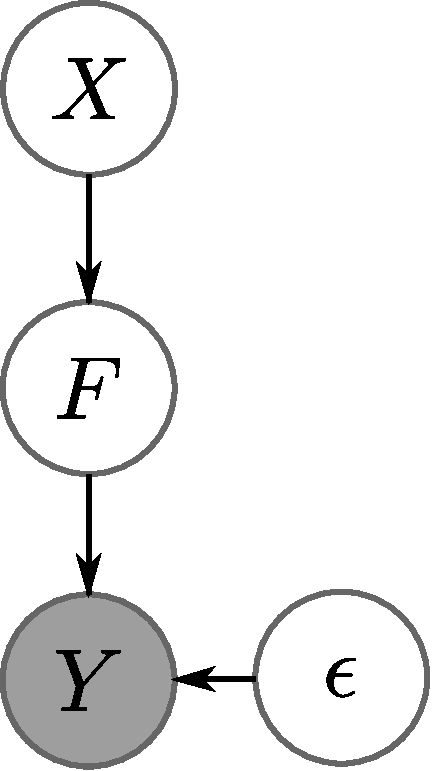
\includegraphics[width=0.12\textwidth]{../diagrams/gplvm}
	\label{fig:gplvm}
}
\hspace{0.1\textwidth}
\subfigure[]{
	\includegraphics[width=0.12\textwidth]{../diagrams/bgplvm}
	\label{fig:bgplvm}
}
\hspace{0.1\textwidth}
\subfigure[]{
	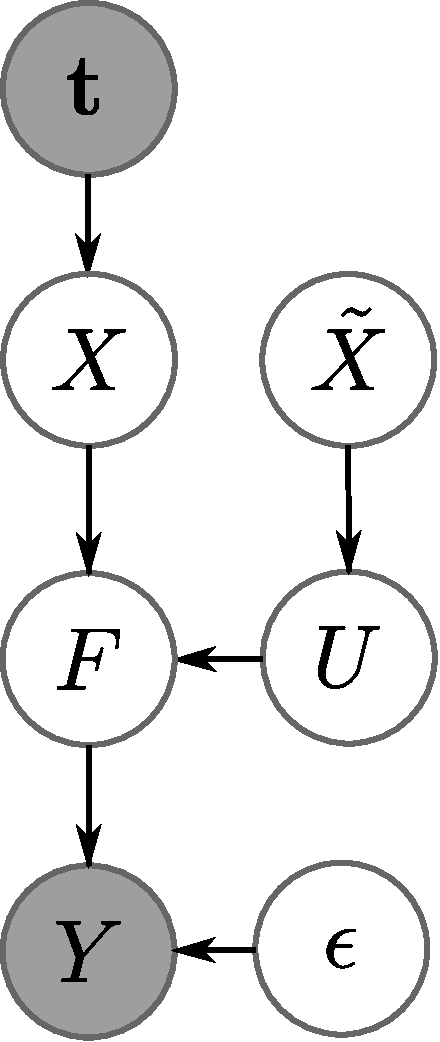
\includegraphics[width=0.12\textwidth]{../diagrams/dbgplvm}
	\label{fig:dbgplvm}
}
\end{center}
\vspace{-8pt}
\caption{ \small{
The graphical model for the standard GP-LVM \subref{fig:gplvm} is augmented with auxiliary variables to obtain the
 Variational GP-LVM model \subref{fig:bgplvm} and its dynamical version \subref{fig:dbgplvm}}.}
\label{fig:graphicalModels}
\end{figure}



%----------------------------------------------- PRIORS ON THE LATENT SPACE ---------------------------------------------------
\subsection{\label{section:priors} Priors On the Latent Space}
% -> Allows to capture assumptions
In the previous section we presented a framework for analytically calculating a variational lower bound on the logarithm of
the marginal likelihood by also integrating the latent space $X$. For this, we did not assume any particular form for the
prior $p(X)$. However, a particular choice for the form of this density greatly reflects our overall modelling assumptions,
it constrains the latent space $X$ and, indirectly, the data space $Y$ (since the model is generative).
\par A simple choice is to assign a standard normal density which factorises across datapoints, as in \cite{BayesianGPLVM}:
\begin{equation}
\label{standardNormal}
p(X) = \prod_{n=1}^N \mathcal{N}(\bfx_n | \mathbf{0}, I_Q) .
\end{equation}

\noindent This prior does not explicitly model correlations between datapoints and, practically, leaves the latent space unconstrainted.
The fact that our model's likelihood breaks into the two terms shown in \eqref{jensensSplit}, means that incorporating this
prior with the variational framework described in section \ref{section:vgplvmBound} only requires two additional, easy steps:
firstly, we have to specify a similar factorisation for $q(X)$, i.e. equation \eqref{qX} can be written in this case as
\begin{equation}
  \label{qXstatic}
  q(X) = \prod_{n=1}^N \mathcal{N}(\bfx_n | \bfmu_n, S_n).
\end{equation} 
Secondly, the corresponding $\text{KL}$ quantity appearing in \eqref{jensensSplit}  has to be calculated, a task which is
almost trivial, especially given that the covariance matrices $S_n$ (in equation \eqref{qXstatic}) are diagonal.
The reason why $S_n$ is used to only model variances, is
that the prior for $X$ is a standard normal distribution, i.e a full independence assumption is made for the latent points.
Of course this is not the best modelling approach when it is known a priori that the corresponding observed datapoints $\bfy_n$
are correlated,
%and that's why in the next section we extend our framework for this scenario.
so in the next section we extend the framework for correlated posteriors.

%..important, let's us capture assumptions about y indirectly...



 % \subsection{Using a Static Prior}


%----------------------------------------------- DYNAMIC PRIOR --------------------------------------------------------------------
\subsection{\label{temporalPrior} Using a Temporal Prior}

%* Note: include figures from the robot demo, showing the visualisation of the latent space with various kernels.
As already discussed in section \ref{section:gplvmDynamics}, a GPLVM-based dynamical model can be obtained by
additionaly including a latent space prior with a temporal component. We can extend the variational framework
described in section \ref{section:vgplvmBound} by showing how to propagate the Gaussian noise throught
the dynamics and the latent space so as to obtain a variational lower bound on the likelihood of such dynamical models.
Our work is focused on the case where the dynamics are regressive (as in, for example, \cite{hgplvm}).
% incorporating dynamics into the standard GP-LVM gives
%a better expressive power to the resulting model, when the application domain is a dynamical system. 
\par Our approach on defining a GPLVM-based dynamical model, is to let
 a {\em temporal} latent function $\bfx(t) \in
 \mathbb{R}^Q$ (with $Q \ll D$) govern the intermediate latent space when generating the data, which are
 now assumed to be a multivariate timeseries $\{\bfy_n,t_n\}_{n=1}^N$. Here, $t_n \in \mathcal{R}_+$ refers to the time at which the datapoint $\bfy_n$ was
 observed. As with the nonlinear mapping $\bff$, the latent function $\bfx$ can be defined as a multivariate Gaussian process,
 so that its functional form can be inferred in a fully Bayesian non-parametric fashion without making strong assumptions.
 More formally, each $\bfy_n$ in equation \eqref{generative} is now produced from $\bfx_n = \bfx(t_n)$, as shown in figure
 \ref{fig:graphicalModels}\subref{fig:dbgplvm}, where:
\begin{equation}
  \label{xt}
  x_q(t)  \sim \mathcal{GP}(0, k_x(t_i,t_j)), \ \ q=1,\ldots,Q .    
\end{equation}

%%%%%%% FIGURE...

\noindent The individual components of the latent function $\bfx$ are taken to be independent sample paths drawn from
a Gaussian process with covariance function $k_x(t_i,t_j)$. This covariance function, parametrised by $\bftheta_x$,
determines the properties of each temporal function $x_q(t)$.
 For instance, the use of an Ornstein-Uhlbeck
covariance function yields a Gauss-Markov process for $x_q(t)$, while
the squared-exponential covariance function gives rise to very smooth and
non-Markovian processes. In our experiments, we will focus on the squared exponential
covariance function (RBF), the Mat\'ern $3/2$ which is only once
differentiable, and a periodic covariance function
\cite{rasmussen-williams, MacKay98} which can be used when data
exhibit strong periodicity. These covariance functions take the form:
\begin{eqnarray}
k_{x(\text{rbf})} \left( \mathit{t_i, t_j} \right) 
& = & \sigma_{\text{rbf}}^2 e^{- \frac{\left( t_i - t_j \right)^2}{\left(
      2l_t^2 \right)}}, 
\ \ k_{x(\text{mat})} \left( t_i, t_j \right) =  
\sigma_{\text{mat}}^2 \left( 1 + \frac{\sqrt{3} |t_i - t_j|}{l_t} \right)
		e^{\frac{ - \sqrt{3} |t_i - t_j|}{l_t} }, \nonumber \\
%\label{matern} 
k_{x(\text{per})} \left( \mathit{t_i, t_j} \right) 
& = & 
	\sigma_{\text{per}}^2 e^{-\frac{1}{2} \frac{\sin^2 \left( \frac{2
                \pi}{T} \left( t_i - t_j \right) \right) }{l_t} }. 
 \label{eq:temporalkernels}
\end{eqnarray}


\par Incorporating a separate GP model for the dynamics is a very convenient way of incorporating any prior information
we may have about the nature of the data. In particular, more sophisticated covariance functions can be constructed
by combining or modifying existing ones. For example, in our experiments we consider a compound covariance function,
$k_{x(\text{per})} + k_{x(\text{rbf})}$
which is suitable for dynamical systems that are known to be only approximately periodic. The first term
captures the periodicity of the dynamics whereas the second one corrects for the divergence
from the periodic pattern by enforcing the datapoints to form smooth trajectories in time.
By fixing the two variances, $\sigma_{\text{per}}^2$ and $\sigma_{\text{rbf}}^2$ to particular ratios, we are able
to control the relative effect of each kernel. Example sample paths drawn from this compound covariance function are
shown in figure \ref{fig:rbfPeriodic}.

\begin{figure}[ht]
\begin{center}
\subfigure[]{
	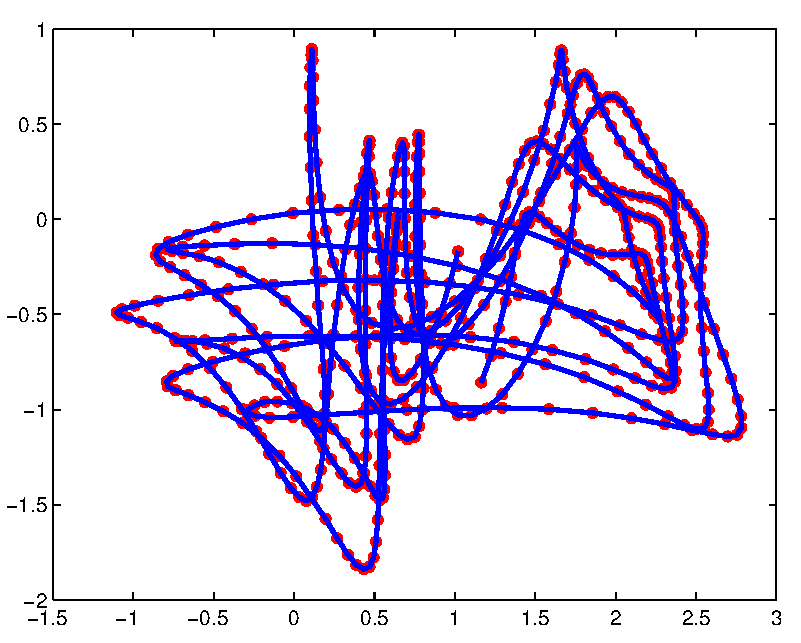
\includegraphics[width=0.31\textwidth]{../diagrams/periodicSamples2}
	\label{fig:rbfPeriodic1}
}
\subfigure[]{
	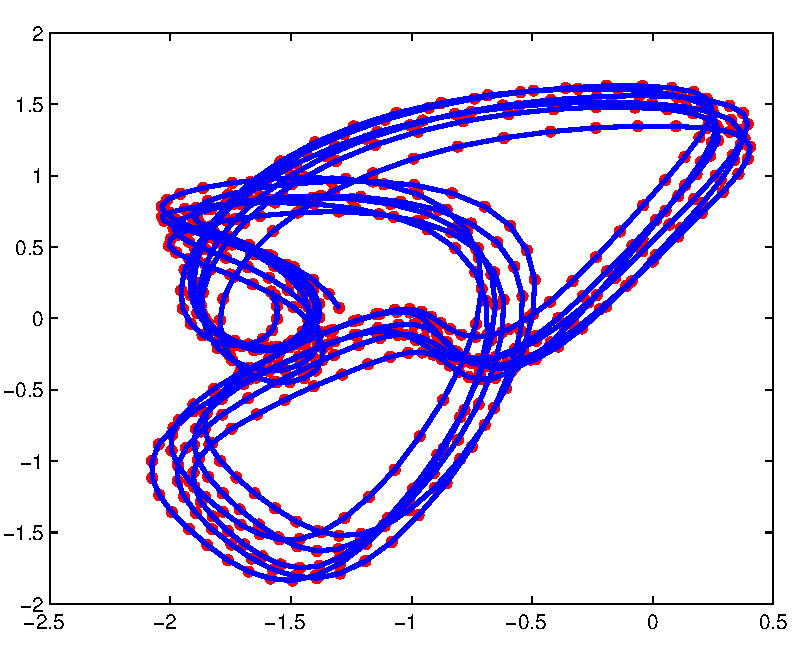
\includegraphics[width=0.31\textwidth]{../diagrams/periodicSamples}
	\label{fig:rbfPeriodic2}
}
\subfigure[]{
	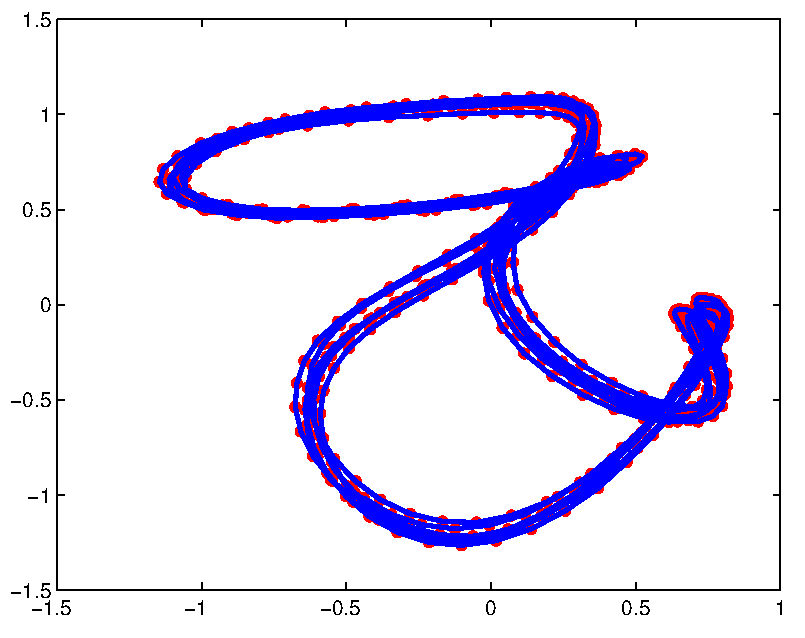
\includegraphics[width=0.31\textwidth]{../diagrams/periodicSamples3}
	\label{fig:rbfPeriodic3}
}
\end{center}
\caption{
  \small{
    Typical sample paths drawn from the $k_{x(\text{per})} + k_{x(\text{rbf})}$ covariance function.
    The variances are fixed for the two terms,
    controlling their relative effect. In figures \subref{fig:rbfPeriodic1}, \subref{fig:rbfPeriodic2} and \subref{fig:rbfPeriodic3},
    the ratio $\sigma_{\text{rbf}}^2 / \sigma_{\text{per}}^2$ of the two variances was large, intermediate and small respectively,
    causing the periodic pattern to be shifted proportionally each period.
  }.
}
\label{fig:rbfPeriodic}
\end{figure}

\noindent After defining a dynamical prior $p(X | \bft)$ as described above, we can then write the marginal GP prior associated with
the temporal function $\bfx$ as
\begin{equation}
p(X | \bft)  = \prod_{q=1}^Q p(\bfx_q|\mathbf{t}) = \prod_{q=1}^Q \mathcal{N} \left( \mathbf{x}_q | \mathbf{0},
  \mathit{K_t} \right),
\label{priorXgivenT}
\end{equation}
\noindent where $K_t = k_x(\bft,\bft)$ is the covariance matrix obtained by
evaluating the covariance function $\mathit{k}_x$ on the observed times
$\bft$. In contrast to the trivial prior \eqref{standardNormal}, the above prior couples datapoints across dimensions and, thus,
the correlations between datapoints can be modelled explicitely in the input space.

\par Bayesian inference using the above model poses a huge computational
challenge and practical approaches that have been considered until now
(e.g. \cite{hgplvm, GPDM}) marginalise out only $F$ and seek a MAP
solution for $X$. However, an approximation to the true marginal likelihood $p(Y|\bft)$ can be found by extending the framework
of section \ref{section:vgplvmBound}, since the form of the bound found there, in equation \eqref{jensensSplit}, only contains the
prior in the $\text{KL}$ quantity as a separate term. Indeed, we can extend our variational framework by first defining a
variational distribution as in \eqref{varDistr}, but now $q(X)$ factorises as:
\begin{equation}
  q(X) = \prod_{q=1}^Q \mathcal{N} \left( \bfx_q | \bfmu_q, S_q \right)
\end{equation}
%
\noindent in accordance with the temporal prior \eqref{priorXgivenT}. Then,
by following exactly the same arguments and derivations,
we can obtain a lower bound in the form of equation \eqref{jensensSplit}. The difference is that the covariance matrices 
$S_q$ are no longer diagonal (like the ones appearing in equation \eqref{qXstatic}); instead, the 
posterior over the latent variables now have strong correlations, so $S_q$ is taken to be a $N \times N$ full covariance
matrix. Therefore, although the $\hat{\mathcal{F}}_v$ term in \eqref{jensensSplit} remains the same for the variational bound of the dynamical GP-LVM model,
the $\text{KL}$ term which contains the prior is now more complicated and harder to compute. More precisely, when not
factorizing $q(X)$ across data points yields $O(N^2)$ variational parameters to optimize. This issue is addressed in the next section.



%\highlight{TODO:} maybe separate section for kernels with images with samples??


%----------------------------------------------- REPARAMETRIZATION AND OPTIMISATION --------------------------------------------
\subsubsection{Reparametrization and Optimization \label{optimisation}} 
%Following \cite{OpperFixedPointCovariance}, we can re-express the variational parameters using $K_t$

A gradient-based algorithm can be employed for training the model, i.e finding the parameters
that maximise the variational lower bound.
This optimization procedure
involves the model parameters $\boldsymbol \theta =
(\beta, \boldsymbol \theta_f, \boldsymbol \theta_x)$, the variational
parameters $\{\mathcal{M}, S \}$ from $q(X)$ and the inducing
points $\tilde{X}$.
%Since $\boldsymbol \theta_f$ and $\boldsymbol \theta_t$ exist in different terms (see \eqref{jensens}), the only coupling between the prior on the latent space (which induces the datapoint correlations) and the likelihood term (which involves observations) is made via the variational parameters. 

% \par In our formulation, unlike \cite{BayesianGPLVM}, the $Q$ variational covariances $S_q$ are full $N \times N$ matrices. 
% Therefore, 
When a temporal prior is used, the optimization of the variational parameters 
$\{ \mathcal{M}, S \} = \{ \bfmu_q, S_q \}_{q=1}^Q$ appears challenging, due to
their large number and the correlations between them. However, by
reparametrizing our $O \left( N^2 \right)$ variational parameters
according to the framework described in
\cite{OpperFixedPointCovariance} we can obtain a set of $O(N)$ less
correlated ones. Specifically, we first take the
derivatives of the variational bound \eqref{jensens1} w.r.t. $S_q$ and
$\bfmu_q$ and set them to zero, to find the stationary
points,
%, one can estimate the variational parameters using fixed-point equations instead of directly optimising them. To obtain such equations we set the variational bound's derivative w.r.t $S_q$ to zero and solve for $S_q$:
\begin{equation}
S_q = \left( \mathit{K}_t^{-1} + \Lambda_q \right)^{-1} \;\;\; \text{and}  \;\;\;  \boldsymbol \mu_q = K_t \bar{\boldsymbol \mu}_q, \label{SFixedPointQ}
\end{equation}
where $\Lambda_q = - 2\frac{\vartheta \mathit{\hat{F}_v(q, \boldsymbol
    \theta)}}{\vartheta \mathit{S_q}}$ is a $N \times N$ diagonal,
positive matrix and $\bar{\boldsymbol \mu}_q = \frac{\vartheta
  \hat{F}_v}{\vartheta \boldsymbol \mu_q}$ is a $N-$dimensional
vector.
%It is now obvious that the variational parameters are correlated,
%since they can be re-expressed as a function of $K_t$. 
The above stationary conditions tell us that, since $S_q$ depends on a
diagonal matrix $\Lambda_q$, we can reparametrize it using only the
$N-$dimensional diagonal of that matrix, denoted by $\boldsymbol
\lambda_q$.  Then, we can optimise the $2 (Q \times N)$ parameters $(
\boldsymbol \lambda_q$, $\bar{\bfmu}_q)$ and obtain the original
parameters using \eqref{SFixedPointQ}.
%One important fact which must be emphasized is that, with the aforementioned methodology, each $\boldsymbol \mu_q$ as well as $S_q$ is now re-parametrised using $K_t$ which means that they now include kernel hyperparameters $\boldsymbol \theta_t$; therefore, the quantity $\frac{\partial \mathbf{F}}{\partial \theta_t}$ should be amended with the partial derivatives as appropriate.





%----------------------------------------------- NUMERICALLY STABLE FORMULATION -----------------------------------------------
%\subsubsection{Numerically stable formulation}
%--> Supplementary
%%%% TODO


%---------------------------------------------- PREDICTIONS ---------------------------------------------------------------------
\section{Predictions \label{section:predictions}} 

%% In this section we explain how the Bayesian models described earlier can be used to achieve various kinds of prediction tasks.
%The predictive tasks associated with the Bayesian models described earlier vary according to the available information of the
%test data and according to whether the model is dynamical or not.
%Firstly, we are interested in finding 
%
%In this section we explain how the Bayesian models described earlier can be used for various kinds of predictive inference.
%...
%p(Y*|Y)
%p(Y*|Y,t) -> The prior gives us info about x*, so we don't have to optimise q(x*) -> generation of data
%p(Y_*^m|Y_*^p,Y)
%...


In this section we explain how the Bayesian models described earlier can accomplish various kinds of predictive tasks which
 concern unobserved, observed or partially observed test data  $Y_* \in \mathcal{R}^{N_* \times D}$.  
In the case where $Y_*$ constitutes a multivariate timeseries, it is additionally associated with with the corresponding timestamps
$\bft_* \in \mathcal{R}^{N_*}$.

\par The first kind of inference discussed here concerns calculating the probability density
 $p(Y_*|Y)$ which can be used as estimator for tasks like generative Bayesian classification. For a test timeseries dataset,
  this density takes the form $p(Y_*|Y,\bft,\bft_*)$. In both cases, test data are allowed to have missing values.
  The later quantity is also of interest when, in contrast to the previously mentioned inference task,
the test sequence $Y_*$ is fully unobserved and needs to be predicted  given only its timestamps $\bft_*$.
 In section \ref{predictions2} we show how this can be achieved.
 Generating novel sequences is a possible task, since our regressive dynamical model corresponds to a
 generative processes (see figure \ref{fig:dbgplvm}).  
 Finally, in section \ref{predictions3}, we explain how we can probabilistically reconstruct 
 partially observed test data  $Y_*^{p} \in \mathbb{R}^{N_* \times D_p}$ from the whole $Y_*
= (Y_*^{p}, Y_*^{m})$, where $p$ and $m$ are set indices indicating
the present (i.e. observed) and missing dimensions of $Y_*$
respectively, so that $p \cup m= \{1,\ldots,D\}$.
 We reconstruct the
missing dimensions of assumingly uncorrelated test data or test timeseries by computing the
 Bayesian predictive distributions $p(Y_*^{m}| Y_*^{p}, Y)$ and $p(Y_*^{m}| Y_*^{p}, Y, \bft, \bft_*)$ respectively.

 \par Whilst time-stamp information is always provided for the dynamical models, in the
next sections we drop its dependence to avoid notational clutter, as it is obvious from the context when the
referred test data $Y_*$ is actually a timeseries.




% If the model is dynamical, then it must be provided with the time-stamps
% $\bft_* \in \mathcal{R}^{N_*}$ of the test points $Y_*$.
% In this case we are interested in computing the density $p(Y_*|Y,\bft,\bft_*)$ and the prediction task can be seen as a data generation process, since the model is requested to produce
% a novel sequence of datapoints given only the associated time vector $\bft_*$. 
% This inference problem is addressed in section \ref{generatingSequences}.
% Finally, in section \ref{partiallyObserved}, we show how a test dataset with partially observed points can be probabilistically reconstructed. 
% ...


\subsection{\label{predictions1} Calculating the density $p(Y_*|Y)$}

We can write the density of interest as the ratio of two marginal likelihoods:

\begin{equation}
\label{pyystar1}
p(Y_*|Y) = \frac{p(Y_*,Y)}{p(Y)} = \frac{\int p(Y_*|Y, X, X_*) p(X,X_*) \intd X \intd X_*}{\int p(Y|X) p(X) \intd X}
\end{equation}
Notice that the denominator constitutes the marginal likelihood of the training data (equation \eqref{marginalLikelihood}) for
the logarithm of which we have already computed the variational lower bound 
$\mathcal{F}_v = \mathcal{F}_v (q(X))$ of equation \eqref{jensensSplit} during training.


As for the numerator of equation \eqref{pyystar1}, its logarithm can be approximated by a variational lower bound
$\mathcal{F}_v^* = \mathcal{F}_v (q(X,X_*))$, which has exactly analogous form to \eqref{marginalLikelihood}. Indeed,
this quantity bounds the logarithm of the marginal likelihood of the training data augmented with the test ones, where
both $X$ and the newly inserted latent variables $X_*$ need to be integrated out. 
Therefore, this bound will now be a function of a variational distribution $q(X,X_*)$
which needs to be optimised so that its marginal $q(X_*)$ approximates the true posterior $p(X_* | Y_*,Y)$.
After this procedure, we will be able to
replace the denominator of \eqref{pyystar1} with $e^{\mathcal{F}_v (q(X,X_*))}$ and the numerator with $e^{\mathcal{F}_v (q(X))}$,
which is treated as a constant in the test phase. We will then be able to approximate the quantity of interest with the equation
\begin{equation}
\label{pyystar2}
p(Y_*|Y) \approx q(Y_*|Y) = e^{\mathcal{F}_v (q(X,X_*)) - \mathcal{F}_v (q(X))}.
\end{equation}

\noindent What now remains is to define the variational distribution 
\begin{equation}
\label{qxxstar}
q(X,X_*) = q(X) q(X_*|X) .
\end{equation}
At this step, the inference procedure
differs depending on the type of prior used for the latent space $X$. The prior \eqref{qXstatic} leaves all the latent points
uncoupled, whereas the dynamical prior \eqref{priorXgivenT} couples the test latent points $\bfx_{n,*}$ with each other as well as with the
training latent points stored in $X$. In the first case, equation \eqref{qxxstar} can be written as 
$q(X,X_*) = \prod_{n=1}^N q(\bfx_n) \prod_{n=1}^{N_*} q(\bfx_{n,*})$, 
where $q(\bfx_{n,*}) = \mathcal{N}(\bfx_{n,*} | \bfmu_{n,*}, S_{n,*})$. 
 This means that we only need to optimise with respect to the $2 (N_* \times Q)$ parameters of $q(X_*)$ 
 (recall that $S_{n,*}$ is a diagonal matrix). 
 The rest of the parameters
on which the variational bound $\mathcal{F}_v(q(X,X_*))$ depend, are held fixed to the values learned during training.
We can perform several precomputations to improve efficiency. In particular, notice that the computation
of the $\Psi$ quantities decomposes across data (as can be seen in the supplementary material and in \cite{BayesianGPLVM})
% \highlight{TODO:(equations for Psis)} 
and therefore, 
%because they only appear in the  ..... . Therefore,
updating
these statistics to account for the insertion of the test point
involves only averages over the factorised variational distribution $q(X_*)$.

\par On the other hand, performing inference in the dynamical model is more challenging, since $q(X,X_*)$ is fully
coupled across $X$ and $X_*$. Therefore, if we wish to maintain the correlation of the inputs depending on their times,
we should select this distribution to only factorise across features: 
$q(X,X_*) = \prod_{q=1}^Q  \mathcal{N} (\bfx_{q,*} | \bfmu_{q,*} ,S_{q,*})$,
 where $S_{q,n}$ are full $(N+N_*) \times (N+N_*)$ matrices which can, however, be reparametrised with $N+N_*$
parameters as discussed in section \ref{optimisation}.
Consequently, the already learned parameters of $q(X)$ cannot be reused. Instead, we must optimise over the whole set of
the $2 \left( Q \times (N + N_*) \right)$ parameters involved in $q(X,X_*)$. A much faster but less
accurate method would be to decouple the test from the training latent variables by imposing the factorisation
$q(X,X_*) = q(X)q(X_*)$, thus assuming that all training and test points are correlated with points only within their own set.
This is not used, however, in our current implementation.

%The variational optimisation will now seek
%to optimise the parameters $\bfmu_{q,*}, S_{q,*}$

%---------------------------------------------- PREDICTIONS given only the test time points ----------------------------------------
\subsection{\label{predictions2} Generating sequences}
This task concerns only the dynamical variational GP-LVM, as this version is able to model the temporal evolution of a dynamical system.
Therefore, it is also able to interpolate or extrapolate new system states.
The predictive density for this problem, $p(Y_*|Y)$ (omitting the dependence on time for simplicity), has the same form as the one
for the task discussed in the previous section. However, here the outputs are totally unobserved and need to be generated given only
their corresponding timestamps and the overall procedure differs in that $q(X_*)$ is now predicted from the GP prior rather than being
optimised.

\par In more detail, to approximate the predictive density, we will need to introduce the underlying latent function
values $F_* \in \mathbb{R}^{N_* \times D}$ (the noisy-free version of $Y_*$) and the latent variables $X_* \in \mathbb{R}^{N_* \times Q}$. We  write the predictive density as
\begin{eqnarray}
p(Y_* | Y) & = & \int p(Y_*, F_*, X_*| Y) \intd  F_* \intd  X_* =  \int p(Y_* | F_*)  p(F_*|X_*, Y) p(X_*|  Y) \intd  F_* \intd  X_* .
\label{eq:predictive1}
\end{eqnarray}
The term $p(F_* |X_*, Y)$ is approximated by the variational distribution
\begin{eqnarray}
q(F_*|X_*) & = & \int \prod_{d \in D} p(\bff_{*,d} | \bfu_d, X_*)  q(\bfu_d) d \bfu_d 
	    = \prod_{d \in D} q(\bff_{*,d} | X_*)  ,
\end{eqnarray}
where $q(\bff_{*,d} | X_*)$ is a Gaussian that can be computed analytically,
since in our variational framework the optimal setting for $q(\bfu_d)$ is also found to be a Gaussian (see suppl. material for complete forms).
%
As for the term $p(X_*| Y)$ in eq. (\ref{eq:predictive1}), it is approximated by
a Gaussian variational distribution $q(X_*)$,
%
\begin{align}
 q(X_*) = \prod_{q=1}^Q q(\bfx_{*,q}) = 
\prod_{q=1}^Q   \int  p(\bfx_{*,q} | \bfx_q) q(\bfx_q) \intd \bfx_q = \prod_{q=1}^Q \la  p(\bfx_{*,q} | \bfx_q) \ra_{q(\bfx_q)} ,\label{qxstar}
\end{align}
%
where $p(\bfx_{*,q} | \bfx_q)$ is a Gaussian found from the conditional GP prior
(see \cite{rasmussen-williams}) and $q(X)$ is also Gaussian. We can, thus, work out analytically the mean and variance 
for \eqref{qxstar}, which turn out to be:
\begin{align}
 \mu_{x_{*,q}} = {}& K_{*N} \bar{\mu}_q \\
  \text{var}(x_{*,q}) = {}& K_{**} - K_{*N} (K_t + \Lambda_q^{-1})^{-1} K_{N*}
\end{align}
where $K_{*N} = k_x(\bft_*, \bft)$, $K_{*N} = K_{*N}^\T$ and $K_{**} = k_x(\bft_*, \bft_*)$. Notice that these equations have
exactly the same form as found in standard GP regression problems.
%
Once we have analytic forms for the posteriors in \eqref{eq:predictive1}, the predictive density is approximated as
%`
\begin{align} 
p(Y_*| Y) {}& \approx  \int p(Y_*| F_*)  q(F_*|X_*) q(X_*) \intd F_* \intd X_* = \int p(Y_* | F_*) \la q(F_* | X_*) \ra_{q(X_*)} \intd F_* , \label{eq:predictive2}
\end{align}
%
which is a non-Gaussian integral that cannot be computed analytically. However, following the same argument as in
\cite{rasmussen-williams, Girard03gaussianprocess}, we can
calculate analytically its mean and covariance:
%Although the expectation appearing in the above integral is not a Gaussian, its moments can be found analytically \cite{rasmussen-williams, Girard03gaussianprocess},
%
\begin{align}
 \mathbb{E}(F_*) ={}&  B^\T \Psi_1^* \label{meanFstar} \\
 \text{Cov}(F_*) ={}& B^\T \left( \Psi_2^* - \Psi_1^* (\Psi_1^*)^\T \right) B + \Psi_0^* I - \text{Tr} \left[ \left( K_{MM}^{-1} - \left( K_{MM} + \beta \Psi_2 \right)^{-1} \right) \Psi_2^* \right] I, \label{covFstar}
\end{align}
%
where $B = \beta \left( K_{MM} + \beta \Psi_2 \right)^{-1} \Psi_1^\T
Y$, $\Psi_0^* = \la k_f(X_*, X_*) \ra$, $\Psi_1^* = \la K_{M*} \ra$
and $\Psi_2^* = \la K_{M*} K_{*M} \ra$. All expectations are taken
w.r.t. $q(X_*)$ and can be calculated analytically, while $K_{M*}$
denotes the cross-covariance matrix between the training inducing
inputs $\tilde{X}$ and $X_*$. The $\Psi$ quantities are calculated analytically (see suppl. material). Finally, since $Y_*$ is just a noisy version of
$F_*$, the mean and covariance of \eqref{eq:predictive2} is just
computed as: $\mathbb{E}(Y_*) = \mathbb{E}(F_*)$ and $\text{Cov}(Y_*)
= \text{Cov}(F_*) + \beta^{-1} I_{N_*}$.

%---------------------------------------------- PREDICTIONS given partially observed otuputs -------------------------------------
\subsection{\label{predictions3} Predictions Given Partially Observed Outputs}

The expression for the predictive density $p(Y_*^m | Y_*^p, Y)$ follows exactly as in section \ref{predictions2} but we
need to compute probabilities for $Y_*^m$ instead of $Y_*$ and $Y$ is replaced with $(Y, Y_*^p)$ in all conditioning sets. Similarly,
$F$ is replaced with $F^m$, and we get:

\begin{equation}
p(Y_*^m | Y, Y_*^p) =  \int p(Y_*^m | F_*^m)  p(F_*^m | X_*, Y, Y_*^p) p(X_*| Y, Y_*^p) \intd  F_*^m \intd  X_* .
\end{equation}

Therefore, similarly to equation \eqref{eq:predictive2}, the left hand side can be approximated with the quantity
\begin{equation}
  \label{eq:predictive3}
  p(Y_*^m | Y, Y_*^p) \approx  \int p(Y_*^m | F_*^m) \la q(F_*^m | X_*) \ra_{q(X_*)} \intd F_*^m .
\end{equation}

Although the above is calculated with the equations \eqref{meanFstar} and \eqref{covFstar} of section \ref{predictions2},
the quantity $q(X,X_*)$ which we first have to find is computed differently than there.

More precisely, instead of finding the variational distribution on the test latent points analytically, we now have to
optimise it (like in section \ref{predictions1}), so that the information in $Y_*^p$ can be taken into account.
This is done by maximising the variational lower bound on the marginal likelihood:
\begin{align}
p(Y_*^p, Y) ={}&  \int p(Y_*^p, Y|X_*, X) p(X_*, X) \intd  X_* \intd  X \nonumber \\
={}&  \int p(Y^m | X) p(Y_*^p, Y^p|X_*, X) p(X_*, X) \intd  X_* \intd  X.  \nonumber
\end{align}
This quantity is bounded by:
\begin{eqnarray}
& & \int q(X_*, X) \log \frac{ p(Y^m | X) 
p(Y_*^p, Y^p|X_*, X) p(X_*,X)}{ q(X_*, X)} \intd  X_* \intd  X \nonumber \\ 
& = & \int q(X) \log p(Y^m | X) \intd  X 
+  \int q(X_*,X) \log p(Y_*^p, Y^p|X_*, X) \intd  X_* \intd  X  \nonumber \\
& - & \text{KL}[q(X_*,X) || p(X_*, X)] \label{partialPredLowerBound}
\end{eqnarray}  
which has exactly analogous form to the bound \eqref{jensensSplit} computed for the training phase
(for simplicity, here we present the form obtained after marginalising $F$). Now, $q(X,X_*)$ is
found exactly with the methods discussed in section \ref{predictions1}, which are also applicable
when $Y_*$ is not fully observed. 






%----------------------------------------------- EXTENSIONS -----------------------------------------------------
\section{\label{section:extensions} Extensions}
%----------------------------------------------- LEARNING FROM MULTIPLE SEQUENCES -----------------------------------------
\subsection{Learning from Multiple Sequences \label{sequences}}

A given data set of multivariate timeseries
may consist of a group of independent observed sequences, each with
a different length (e.g.\ in human motion capture data several walks
from a subject). Let, for example, the dataset be a group of
$S$ independent sequences  $\left( Y^{(1)}, ..., Y^{(S)} \right)$. We would like the dynamical version of our
model to capture the underlying
commonality of these data. We handle this by allowing a different temporal latent function for each of the independent
sequences, so that $X^{(s)}$ is the set of latent variables corresponding to the sequence $s$.
%so that there are different sets of latent variables $X^{(s)}$ within a shared latent space. 
%
These sets are a priori assumed to be independent since they correspond to separate sequences,
i.e.\ $p\left( X^{(1)}, X^{(2)}, ..., X^{(S)} \right) = \prod_{s=1}^S p(X^{(s)})$, where we dropped the
conditioning on time for simplicity.
%These sets are a priori assumed to be
%independent, i.e.\ $p\left( X^{(1)}, X^{(2)}, ..., X^{(S)} \right) = \prod_{s=1}^S p(X^{(s)})$, where we dropped the
%conditioning on time for simplicity.
%
This factorisation leads to a block-diagonal structure for the time covariance matrix $K_t$, where each block corresponds to one sequence.
 In this setting, each block of observations $Y^{(s)}$ is generated from its corresponding $X^{(s)}$
according to $Y^{(s)} = F^{(s)} + \boldsymbol \epsilon$, where the latent function which governs this mapping is shared across all sequences and 
$\boldsymbol \epsilon$ is Gaussian noise. 


%----------------------------------------------- HANDLING VERY HIGH DIMENSIONAL DATA -----------------------------------------
\subsection{Handling Very High Dimensional Datasets}

Our variational framework avoids the typical cubic complexity of
Gaussian processes allowing relatively large training sets (thousands
of time points, $N$). Further, the model scales only linearly with the
number of dimensions $D$. Specifically, the number of dimensions only
matters when performing calculations involving the data matrix $Y$. In
the final form of the lower bound (and consequently in all of the
derived quantities, such as gradients) this matrix only appears in the
form $Y Y^\T$ which can be precomputed. This means that, when $N \ll
D$, we can calculate $Y Y^\T$ only once and then substitute $Y$ with
the SVD (or Cholesky decomposition) of $Y Y^\T$. In this way, we can
work with an $N \times N$ instead of an $N \times D$
matrix. Practically speaking, this allows us to work with data sets
involving millions of features. In our experiments we model directly
the pixels of HD quality video, exploiting this trick.



%\section{Initialisation ...?}

%----------------------------------------------- MATLAB SCRIPT ------------------------------------------------------------
%------------------------- This is the embedded MATLAB script ------------%
\begin{matlab}
%}
% Demos: Reproduce all results and plots used for the VGPDS 2011 paper.
% COPYRIGHT : Andreas C. Damianou, 2011

% VARGPLVM

% Clear memory and close figures
clear all
close all

% If this variable is set to one, then all the models will be retrained, no
% stored results will be used, everything will be computed from the
% beginning. This might take a log of time though. It this variable is set
% to zero, then the precomputed model will be loaded. In that case,however,
% the precomputed results should be included in the path as .mat files.
retrainModels = 0;

% Like the global above, by setting this to 1 you can repeat only the test
% phase, provided that the .mat files for the training phase (the trained
% model) is included in the path. Again, this needs a lot of time but, of
% course, it's better than also retraining the model.
rePredict = 0;

% Note: if both retrainModels and rePredict are set to zero, then the
% precomputed results are loaded an the program just prints the plots.

% Save the above options because the script clears the workspace
save 'opts.mat' 'retrainModels' 'rePredict'
system('mkdir ../diagrams');
%% 

% ########################## OCEAN ######################################
%{
% Note: The ocean demo is optimised so that we work with an NxN matrix
% instead of an NxD. However, this is done for the long optimisation
% procedure. For quick tasks (posteriorMeanVar, NN predictions) and for the
% plots we work with the full matrix. However, it is so large that regular
% machines cannot load at once. This can be fixed (e.g. to process the
% matrices in parts) easily or we can work on the server machine. For the
% plots, at least, we need the full matrix in any case.
clear; load opts
fprintf(1,'\n\n#-----  OCEAN DEMO ----#\n');
dataSetName = 'ocean';
experimentNo=60;
indPoints=-1; latentDim=20;
fixedBetaIters=200; reconstrIters = 2000;
itNo=[1000 2000 5000 8000 4000];
dynamicKern={'rbf','white','bias'};
whiteVar = 0.1;  vardistCovarsMult=1.7;
dataSetSplit = 'randomBlocks';
if retrainModels
    demHighDimVargplvm3
elseif rePredict
    demHighDimVargplvmTrained
else
    load demOceanVargplvm60Pred
    demHighDimVargplvmLoadPred
end
% Produce plots
fr=reshape(Varmu(27,:),height,width); imagesc(fr); colormap('gray'); % VGPDS
print -depsc oceanGpdsframe27.eps; system('epstopdf oceanGpdsframe27.eps');
fr=reshape(NNmuPartBest(27,:),height,width); imagesc(fr); colormap('gray'); % NN
print -depsc oceanNNframe27.eps; system('epstopdf oceanNNframe27.eps');
%}
%%

% ############################ MISSA ###################################
clear; load opts
fprintf(1,'\n\n#-----  MISSA DEMO ----#\n');
experimentNo = 59;
dataSetName = 'missa';
indPoints = -1; latentDim=25;
fixedBetaIters=50; reconstrIters = 4000;
itNo=[1000 2000 5000 8000 2000]; % 18000
dynamicKern={'matern32','white','bias'};
vardistCovarsMult=1.6;
dataSetSplit = 'blocks';
blockSize = 4; whiteVar = 0.1;
msk = [48 63 78 86 96 111 118];
if retrainModels
    demHighDimVargplvm3
elseif rePredict
    demHighDimVargplvmTrained
else
    load demMissaVargplvm59Pred
    demHighDimVargplvmLoadPred
end

% Produce plots
fr=reshape(Varmu(46,:),height,width); imagesc(fr); colormap('gray'); % VGPDS
print -depsc missaGpdsframe46.eps; system('epstopdf missaGpdsframe46.eps');
fr=reshape(YtsOriginal(46,:),height,width); imagesc(fr); colormap('gray'); % Original
print -depsc missaYtsOrigframe46.eps; system('epstopdf missaYtsOrigframe46.eps');
fr=reshape(NNmuPartBest(46,:),height,width); imagesc(fr); colormap('gray'); % NN for best k
print -depsc missaNNframe46.eps; system('epstopdf missaNNframe46.eps');
% The following two pictures are edited in the paper so that they fit in
% the place of one single picture
fr=reshape(Yts(17,:),height,width); imagesc(fr); colormap('gray'); 
print -depsc missaGpdsPredFrame17_part1.eps; system('epstopdf missaGpdsPredFrame17_part1.eps');
fr=reshape(Varmu(17,:),height,width); imagesc(fr); colormap('gray');
print -depsc missaGpdsPredFrame17_part2.eps; system('epstopdf missaGpdsPredFrame17_part2.eps');
%%


% ############################ DOG #######################################

%------------ GENERATION -------
% Train
clear; load opts
fprintf(1,'\n\n#-----  DOG DEMO: Generation ----#\n');
dataSetName = 'dog';
experimentNo=61;
indPoints=-1; latentDim=35;
fixedBetaIters=400;
reconstrIters = 1; % no reconstruction needed here
itNo=[1000 1000 1000 1000 1000 1000 500 500 500 500 1000 1000 1000 1000 1000 1000 1000 500 500]; %16000
periodicPeriod = 4.3983; % Recalculated for dataToKeep=60
dynamicKern={'rbfperiodic','whitefixed','bias','rbf'};
vardistCovarsMult=0.8;
whiteVar = 1e-6;
dataToKeep = 60; dataSetSplit = 'custom';
indTr = [1:60];
indTs = 60; % We don't really reconstruct in this experiment
learnSecondVariance = 0;
if retrainModels
    demHighDimVargplvm3
end

%-- Then generate:
clear; load opts; close all 
dataSetName = 'dog'; 
experimentNo=61; dataToKeep = 60; dataSetSplit = 'custom';
indTr = [1:60]; indTs = 60;
futurePred = 40; doSampling = 0; demHighDimVargplvmTrained
%clear Yts; clear YtsOriginal; clear Testmeans2; clear Testcovars2;
%playMov(height, width, [], [Ytr(end-5:end,:); Varmu2]);

% Produce plots
bar(prunedModelInit.kern.comp{1}.inputScales)
print -depsc dog_scalesInit.eps; system('epstopdf dog_scalesInit.eps');
bar(model.kern.comp{1}.inputScales)
print -depsc dog_scalesOpt.eps; system('epstopdf dog_scalesOpt.eps');

fr=reshape(Ytr(end,:),height,width); imagesc(fr); colormap('gray'); % Last training image
print -depsc dogGeneration_lastOfTraining.eps; system('epstopdf dogGeneration_lastOfTraining.eps');
fr=reshape(Varmu2(1,:),height,width); imagesc(fr); colormap('gray');  % First predicted
print -depsc dogGeneration_firstOfTest.eps; system('epstopdf dogGeneration_firstOfTest.eps');
fr=reshape(Varmu2(13,:),height,width); imagesc(fr); colormap('gray'); % A subsequent frame
print -depsc dogGeneration_frame14.eps; system('epstopdf dogGeneration_frame14.eps');


% The following is for interpolation
%dt = 0.103; subs=4; futurePred = 0:(dt/subs):(dt/subs)*(size(Ytr,1)-1)*subs; 
%demHighDimVargplvmTrained
%playMov(height, width, [0.03 subs], Varmu2, Ytr );

%%

%--------- Reconstruction
% Train
clear; load opts
fprintf(1,'\n\n#-----  DOG DEMO: Reconstruction ----#\n');
dataSetName = 'dog';
experimentNo=65;
indPoints=-1; latentDim=35;
fixedBetaIters=400;
reconstrIters = 2;
itNo=[1000 1000 1000 1000 1000 1000 500 500 500 500 1000 1000 1000 1000 1000 1000 1000 500 500]; %16000
periodicPeriod = 2.8840;
dynamicKern={'rbfperiodic','whitefixed','bias','rbf'};
vardistCovarsMult=0.8;
whiteVar = 1e-6;
dataSetSplit = 'custom';
indTr = 1:54;
indTs = 55:61;
learnSecondVariance = 0;
if retrainModels
    demHighDimVargplvm3
end

%%

% Test
clear; load opts
dataSetName = 'dog';
experimentNo=65;
dataSetSplit = 'custom';
indTr = 1:54; indTs = 55:61;
predWithMs = 1; % Do reconstruction
reconstrIters = 18000; 
doSampling = 0;
if rePredict
    demHighDimVargplvmTrained
else
    load demDogVargplvm65Pred
    demHighDimVargplvmLoadPred
end
% Produce plots (these go to the supplementary)
fr=reshape(Varmu(5,:),height,width); imagesc(fr); colormap('gray'); 
print -depsc supplDogPredGpds5.eps; system('epstopdf supplDogPredGpds5.eps');
fr=reshape(Yts(5,:),height,width); imagesc(fr); colormap('gray'); 
print -depsc supplDogPredYts5.eps; system('epstopdf supplDogPredYts5.eps');
fr=reshape(Varmu(6,:),height,width); imagesc(fr); colormap('gray'); 
print -depsc supplDogPredGpds6.eps; system('epstopdf supplDogPredGpds6.eps');
fr=reshape(Yts(6,:),height,width); imagesc(fr); colormap('gray'); 
print -depsc supplDogPredYts6.eps; system('epstopdf supplDogPredYts6.eps');

%%

% ############################ CMU ###################################
%rbf
clear; load opts
fprintf(1,'\n\n#-----  CMU DEMO: Rbf ----#\n');
experimentNo=34; 
itNo = [300 300 400 200 200 300 400 400];
dynamicKern = {'rbf', 'white', 'bias'};
vardistCovarsMult = 0.152;
if retrainModels 
    if rePredict
        doReconstr = 1;
    else
        doReconstr=0;
    end
    demCmu35gplvmVargplvm3;
elseif rePredict
    % 'demCmu35gplvmVargplvm34.mat' must be included in the path
    demCmu35vargplvmReconstructTaylor
end
predictPart = 'Legs';  plotRange = [];
demCmu35VargplvmPlotsScaled
% demCmu35VargplvmAnimate
fprintf(1,'# VGPDS RBF error on Legs reconstr:');
errStruct

predictPart = 'Body';  plotRange = [];
demCmu35VargplvmPlotsScaled
% demCmu35VargplvmAnimate
fprintf(1,'# VGPDS RBF error on Body reconstr:');
errStruct

bar(model.kern.comp{1}.inputScales);
print -depsc supplMocapScalesRbf.eps; system('epstopdf supplMocapScalesRbf.eps');


% matern32 for legs
clear; load opts
fprintf(1,'\n\n#-----  CMU DEMO: Matern32 ----#\n');
experimentNo=33; 
itNo = [300 300 400 200 200 300 400 400];
dynamicKern = {'matern32', 'white', 'bias'};
vardistCovarsMult = 0.24;
if retrainModels 
    if rePredict
        doReconstr = 1;
    else
        doReconstr=0;
    end
    demCmu35gplvmVargplvm3;
elseif rePredict
    % 'demCmu35gplvmVargplvm33.mat' must be included in the path
    demCmu35vargplvmReconstructTaylor
end
predictPart = 'Legs'; plotRange = 10;
demCmu35VargplvmPlotsScaled
print -depsc supplMocapLeg5GpdsMatern.eps; system('epstopdf supplMocapLeg5GpdsMatern.eps');
% demCmu35VargplvmAnimate
fprintf(1,'# VGPDS Matern error on Legs reconstr:');
errStruct

predictPart = 'Body'; plotRange = 28;
demCmu35VargplvmPlotsScaled
print -depsc supplMocapBody28GpdsMatern.eps; system('epstopdf supplMocapBody28GpdsMatern.eps');
% demCmu35VargplvmAnimate
fprintf(1,'# VGPDS Matern error on Body reconstr:');
errStruct
close all
bar(model.kern.comp{1}.inputScales);
print -depsc supplMocapScalesMatern.eps; system('epstopdf supplMocapScalesMatern.eps');


%% ---------
fprintf(1,'\n\n#---- FINISHED reproducing plots and results!! \n');
delete opts.mat


% Record version of MATLAB/Octave
a = ver('octave');
if length(a) == 0
  a = ver('matlab');
end
fid = fopen('vers.tex', 'w');
fprintf(fid, [a.Name ' version ' a.Version]);
fclose(fid);

% Record computer architecture.
fid = fopen('computer.tex', 'w');
fprintf(fid, ['\\verb+' computer '+']);
fclose(fid);

% Record date of run.
fid = fopen('date.tex', 'w');
fprintf(fid, datestr(now, 'dd/mm/yyyy'));
fclose(fid);

%{
\end{matlab}
%------------------------------------------------------------------% % This is the embedded matlab script





%------------------------------------------------ EXPERIMENTS --------------------------------------------------------
\section{\label{section:experiments} Experiments}

The experiments presented in this section are intended to explore the various properties of both, the Variational
GP-LVM as well as its dynamical version. The most important of these properties include the generative Bayesian
nature of our models, the ability to handle very high dimensional data as well as the automatic way of determining
the complexity and performing model selection.

Therefore, we evaluate the models' performance in a variety of tasks, namely
visualisation, prediction, reconstruction and generation of data or timeseries.
Matlab source code for repeating the following experiments is available
on-line from: \\
\verb|http://staffwww.dcs.shef.ac.uk/people/N.Lawrence/vargplvm/|.

\subsection{Visualisation tasks}

Given a dataset with known structure, we can apply our algorithm and evaluate its performance in a simple and intuitive
way, by checking if the form of the discovered low dimensional manifold agrees with our prior knowledge.
%In this section we present two experiments of this kind. 
\par
%Firstly, we 
We
illustrate the method in the multi-phase oil
flow data \cite{Bishop:oil93} that consists of $1000$, $12$ 
dimensional observations belonging to three known classes
corresponding to different phases of oil flow.   
Figure \ref{fig:oil} shows the results for these  data obtained
by applying the Bayesian GP-LVM with $10$ latent dimensions using the ARD SE
kernel. The means of the variational distribution were initialized
based on PCA, while the variances in the variational distribution are 
initialized to neutral values around $0.5$. As shown in Figure
\ref{fig:oilScales}, the algorithm switches
off automatically $7$ out of $10$ latent dimensions by making their 
inverse lengthscales zero. Figure \ref{fig:oilBGPLVM} shows the
visualization obtained by keeping only the 
dominant latent directions (having the largest inverse lengthscale)
which are the dimensions $2$ and $3$. This is a remarkably high quality two
dimensional visualization of this data. For comparison, Figure
\ref{fig:oilGPLVM} shows the visualization provided by the standard sparse
GP-LVM that runs by assuming only $2$ latent dimensions. 
Both models use $50$ inducing variables, while the latent variables
$X$ optimized in the standard GP-LVM are initialized based on PCA. 
Note that if we were to run the standard GP-LVM with $10$ latent 
dimensions, the model would overfit the data, it would not reduce the 
dimensionality in the manner achieved by the Bayesian GP-LVM. In these 
two dimensions, the nearest neighbour error for the different classes 
(phases of oil flow) in the case of Bayesian GP-LVM is 3 errors from
$1000$ data points. The number of the nearest neighbour errors made
when applying the standard GP-LVM was $26$. 

%%% TODO %%%%
%Due to the curse of dimensionality, it is often difficult to recognise the structure of high dimensional data, even if there is some.
%A dimensinoality reduction algorithm can be useful for visualising this kind of data, so that we can gain some intuition about their nature.
%This is achieved by visualising a low dimensional, non-linear projection of the data. 
%Reversely, given a dataset with known structure, we can apply our algorithm and evaluate its performance in a simple and intuive way by checking if the shape of the discovered low dimensional manifold agrees with our prior knowledge. 
%
%In this section we present two experiments of this kind. Most of the existing approaches cannot ... so they set by hand 2 or 3 latent dims...
%advantage of vargplvm to find the number of latent dims...
%%%%



\begin{figure}[ht]
\begin{center}
\subfigure[]{
	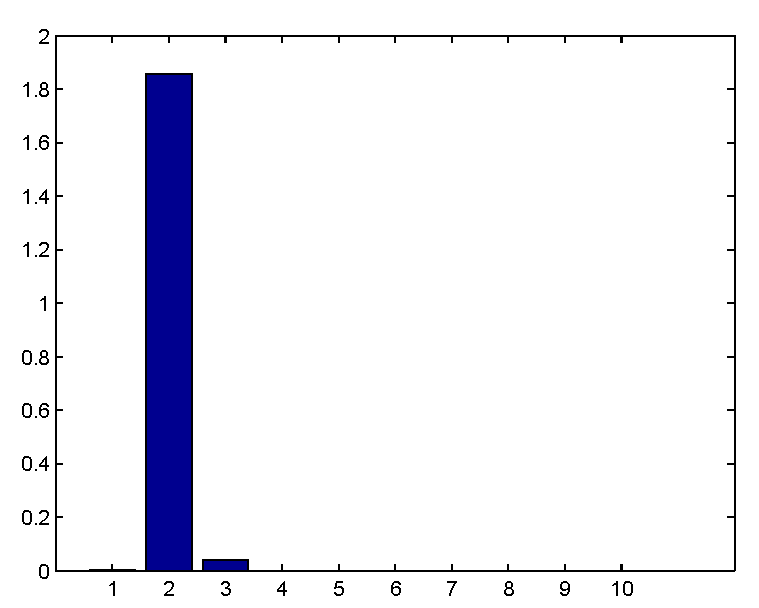
\includegraphics[width=0.31\textwidth]{../diagrams/demOilVargplvm1Scales.pdf}
	\label{fig:oilScales}
}
\subfigure[]{
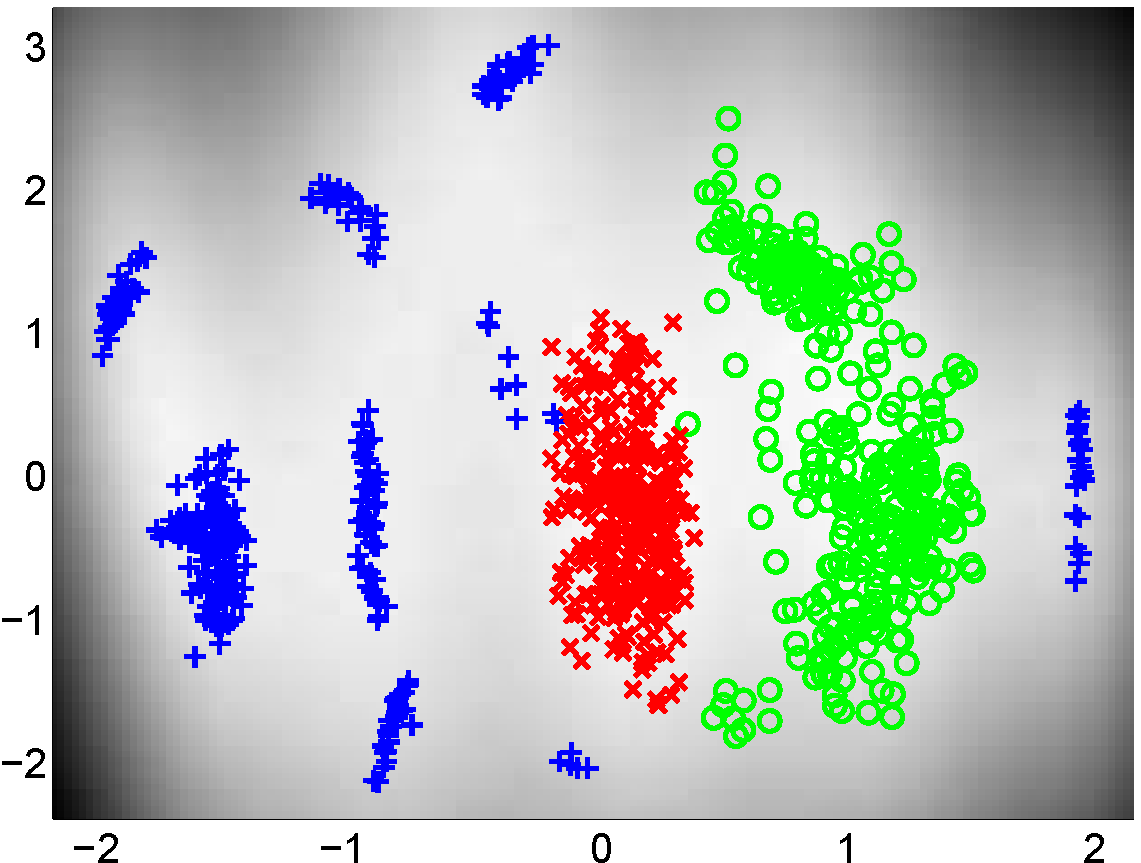
\includegraphics[width=0.31\textwidth]{../diagrams/demOilVargplvm1.pdf}
	\label{fig:oilBGPLVM}
}
\subfigure[]{
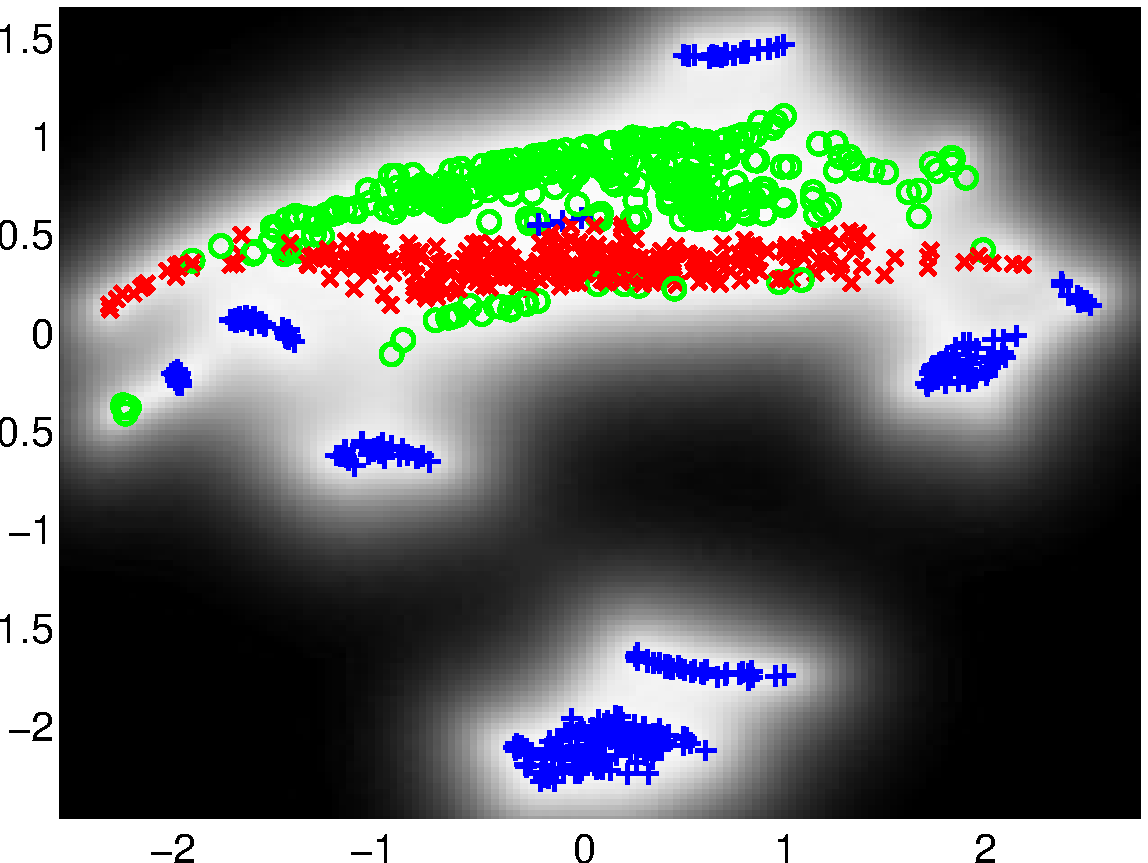
\includegraphics[width=0.31\textwidth]{../diagrams/demOilFgplvm7.pdf}
	\label{fig:oilGPLVM}
}
\end{center}
\caption{\small{
 Panel (a) shows the inverse lengthscales found by applying the
  Bayesian GP-LVM with ARD SE kernel on the oil flow data. Panel (b)
  shows the visualization achieved by keeping the most dominant latent
  dimensions (2 and 3) which have the largest inverse lengthscale
  value. Dimension 2 is plotted on the
  $y$-axis and 3 and on the $x$-axis. Plot (c) shows the visualization found
  by standard sparse GP-LVM.
}
}
\label{fig:oil}
\end{figure}

%%%%%%%% TODO
%\par As a second visualisation task, 
%
%\begin{figure}[ht]
%\begin{center}
%\subfigure[]{
%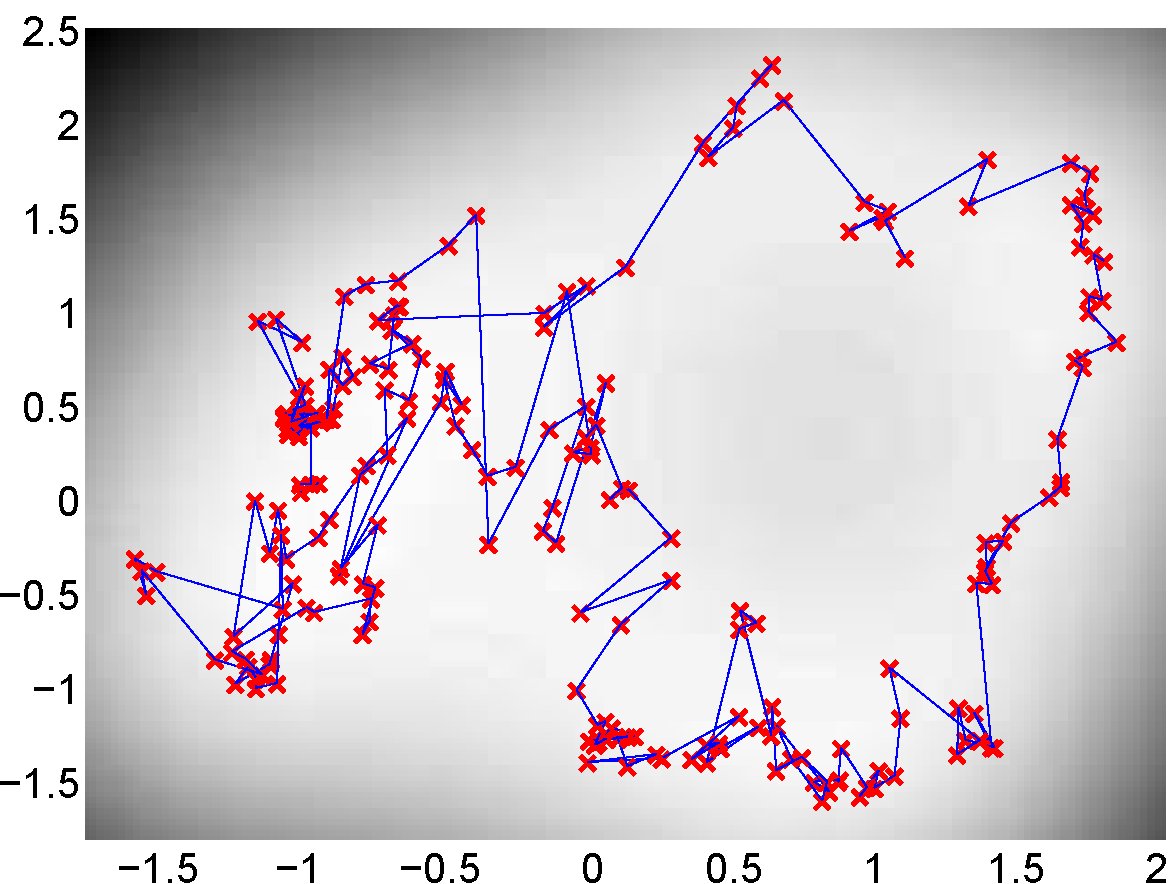
\includegraphics[width=0.45\textwidth]{../diagrams/demRobotWirelessVargplvmStatic.pdf}
%	\label{fig:robotStatic}
%}
%\subfigure[]{
%	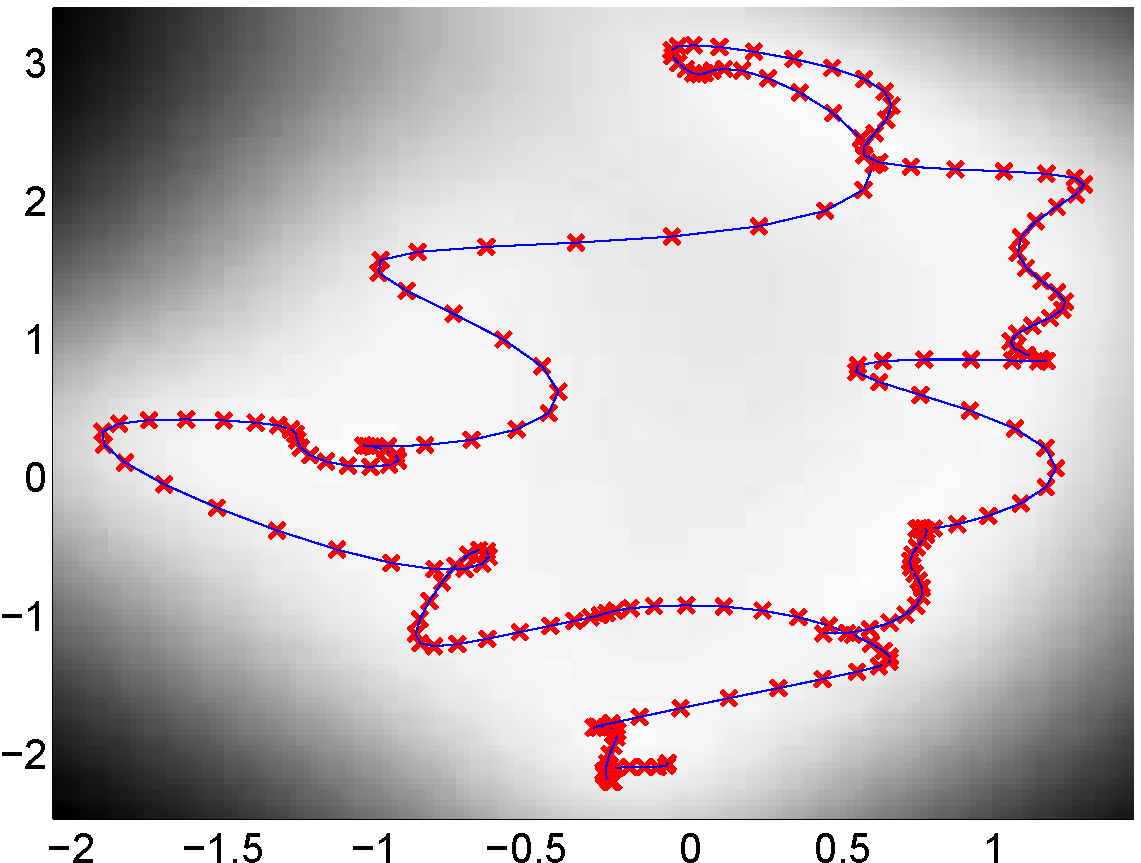
\includegraphics[width=0.45\textwidth]{../diagrams/demRobotWirelessVargplvmDynRbf.pdf}
%	\label{fig:robotDyn}
%}
%\end{center}
%\caption{\small{
%    Loop closure in robotics. \subref{fig:robotStatic}: var. gplvm without dynamics. \subref{fig:robotDyn}: var. gplvm with an RBF kernel to model the dynamics....
%}
%}
%\label{fig:robot}
%\end{figure}

\subsection{Human Motion Capture Data}

We followed \cite{Taylor,gplvmLarger} in considering motion capture
data of walks and runs taken from subject 35 in the CMU motion capture
database. We used the dynamical version of our model and
treated each motion as an independent sequence.  The data
set was constructed and preprocessed as described in
\cite{gplvmLarger}. This results in 2,613 separate 59-dimensional
frames split into 31 training sequences with an average length of 84
frames each. Our model does not require explicit timestamp information, since we
know a priori that there is a constant time delay between poses and the model can construct
equivalent covariance matrices given any vector of equidistant time points.

The model is jointly trained, as explained in section \ref{sequences},
on both walks and runs, i.e. the algorithm learns a common latent
space for these motions. At test time we investigate the ability of
the model to reconstruct test data from a previously unseen sequence
given partial information for the test targets. This is tested once by
providing only the dimensions which correspond to the body of the
subject and once by providing those that correspond to the legs.
%
We compare with results in \cite{gplvmLarger}, which used MAP
approximations for the dynamical models, and against nearest
neighbour. We can also indirectly compare with the binary latent
variable model (BLV) of \cite{Taylor} which used a slightly different
data preprocessing. Furthermore, we additionally tested the non-dynamical
version of our model, in order to explore the structure of the distribution found for the
latent space. In this case, the notion of sequences or sub-motions is not modelled
explicitely, as the non-dynamical approach does not model correlations between
datapoints. However, as will be shown below, the model manages to discover
the dynamical nature of the data and this is reflected in both, the structure of
the latent space and the results obtained on test data.

\par The performance of each method is assessed by using the cumulative
error per joint in the scaled space defined in \cite{Taylor} and by
the root mean square error in the angle space suggested by
\cite{gplvmLarger}. Our models were initialized with nine latent
dimensions. For the dynamical version, we performed two runs, once using the Mat\'ern covariance
function for the dynamical prior and once using the RBF.

%
The appropriate latent space dimensionality for the data was
automatically inferred by our models. 
%If an RBF covariance governed
%the dynamics the model retained four dimensions, whereas the model
%that used the Matern kept only three.
The non-dynamical model
discovered a $5$-dimensional latent space.
The model which employed an Mat\'ern covariance to govern the dynamics retained four dimensions,
whereas the model that used the RBF kept only three. 
%
%The
%models automatically inferred that the
%appropriate latent space dimensionality for the data was three. 
%
The other latent dimensions were completely switched off by the ARD
parameters.



 From table
\ref{motionCaptureTable} we see that the dynamical Variational GP-LVM
considerably outperforms the other approaches.
The best performance for the legs and the body
reconstruction was achieved by the VGPDS model that used the Mat\'ern
and the RBF covariance function respectively. This is an intuitive result, since the smoother
body movements are expected to be better modelled using the infinite differentiable
RBF covariance function, whereas the Mat\'ern one can easier fit the rougher leg motion.
However, although it is important to take into account any available information about the nature of
the data, the fact that both models outperform significantly other approaches shows that the Bayesian
training manages successfully to fit the covariance function parameters to the data in any case.
%
%It is also worth mentioning that  \highlight{TODO:likelihood}
%
Furthermore, the non-dynamical variational GP-LVM, not only manages to discover a latent space with a dynamical
structure, as can be seen in figure \ref{fig:cmuLatentSpaceStatic}, but is also proven to be very robust when making predictions. Indeed,
table \ref{motionCaptureTable} shows that the non-dynamical variational GP-LVM typically outperforms Nearest Neigbour
and its performance is comparable to the GP-LVM which explicitely models dynamics but uses MAP approximations.




%The best performance for legs reconstruction was achieved by the model using the Matern covariance whereas the best performance for body reconstruction used the RBF.
\begin{figure}[ht]
\begin{center}
\subfigure[]{
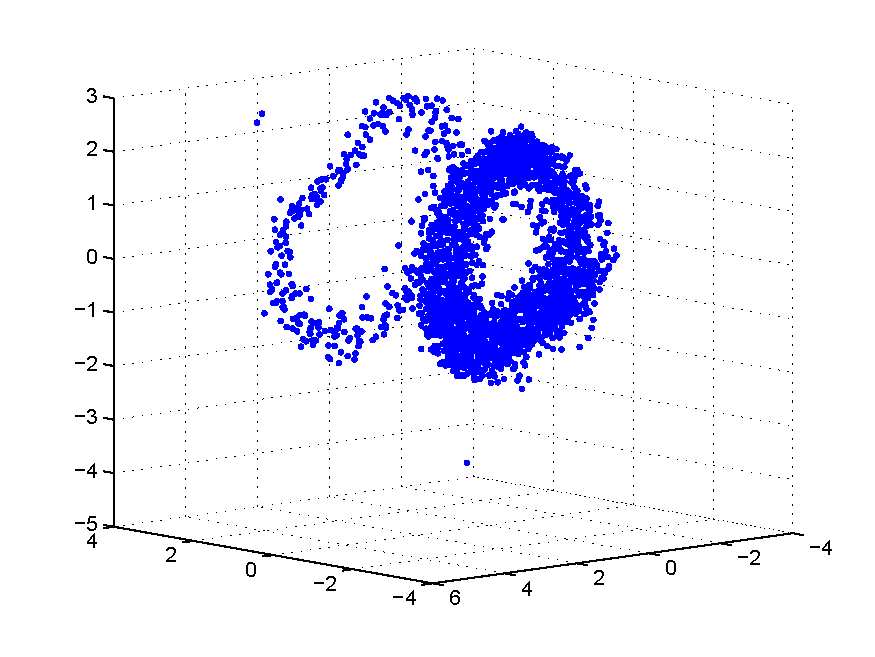
\includegraphics[width=0.31\textwidth]{../diagrams/demCmuStaticLatentSpaceX123}
	\label{fig:cmuLatentSpaceStatic}
}
\subfigure[]{
	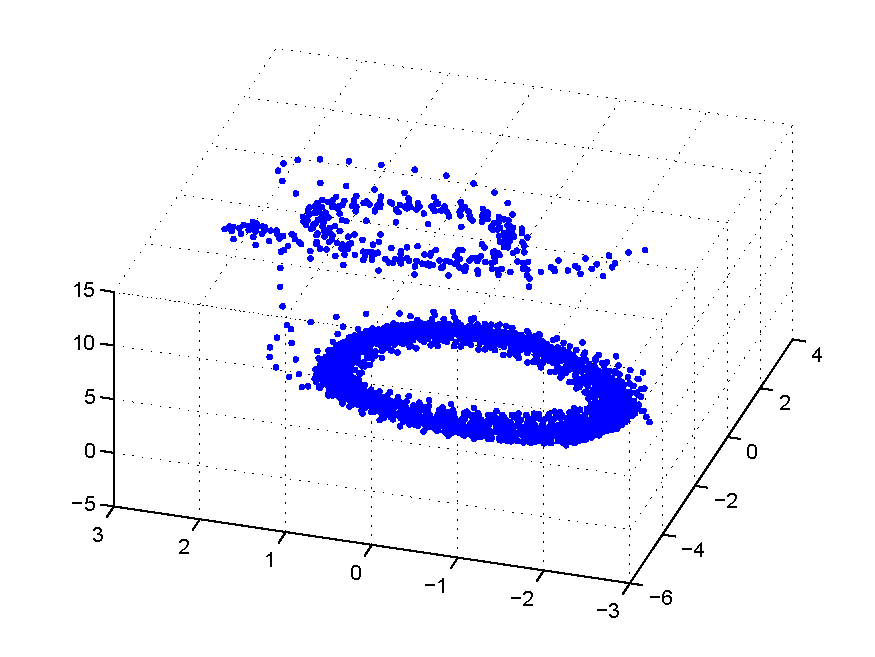
\includegraphics[width=0.31\textwidth]{../diagrams/demCmuMaternLatentSpace}
	\label{fig:cmuLatentSpaceMatern}
}
\subfigure[]{
	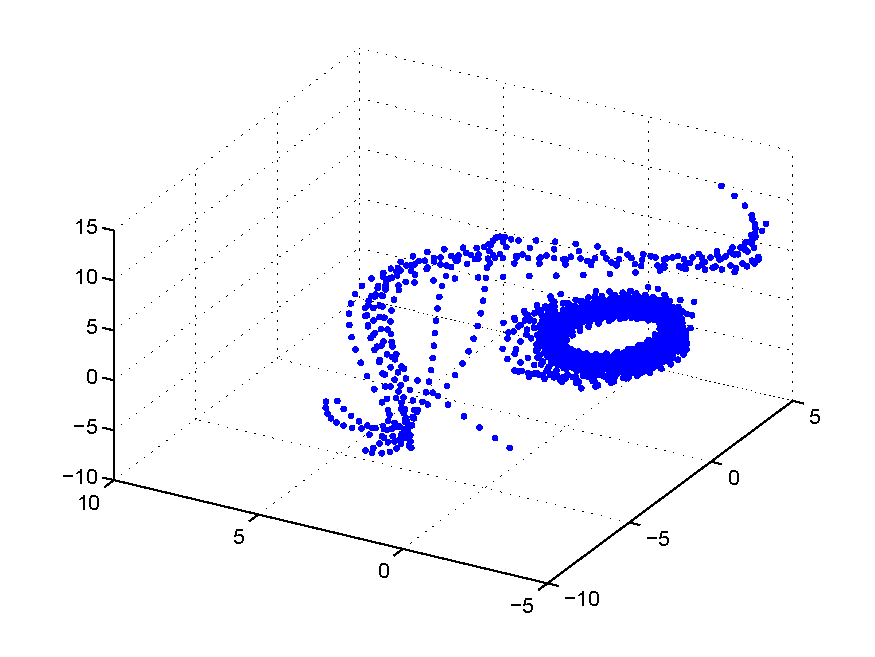
\includegraphics[width=0.31\textwidth]{../diagrams/demCmuRbfLatentSpace}
	\label{fig:cmuLatentSpaceRbf}
}
\end{center}
\caption{\small{
The latent space discovered by our models, projected into its three principle dimensions. The latent space found by the
non-dynamical Bayesian GP-LVM is shown in \subref{fig:cmuLatentSpaceStatic}, by the dynamical model which uses the
Mat\'ern in \subref{fig:cmuLatentSpaceMatern} and by the dynamical model which uses the RBF in \subref{fig:cmuLatentSpaceRbf}.
}
}
\label{fig:cmuLatentSpaces}
\end{figure}


\begin{table}[h]
\caption{
\small{
Errors obtained for the motion capture dataset considering nearest neighbour in the angle space (NN) and in the scaled space(NN sc.), GPLVM, BLV, Variational GPLVM (VGPLVM) and Dynamical VGPLVM (Dyn. VGPLVM). CL / CB are the leg and body datasets as preprocessed in \cite{Taylor}, L and B the corresponding datasets from \cite{gplvmLarger}. SC corresponds to the error in the scaled space, as in Taylor et al. while RA is the error in the angle space. The best error per column is in bold. }}
\label{motionCaptureTable}
\begin{center}
\begin{tabular}{c||c|c|c|c|c|c}
%\multicolumn{1}{c}{\bf PART}  &\multicolumn{1}{c}{\bf DESCRIPTION}
Data & CL & CB & L & L & B & B \\  \hline
Error Type & SC & SC & SC & RA & SC & RA \\
\hline \hline
BLV 			       & 11.7 & \textbf{8.8} & - & - & - & - \\  \hline
NN sc.   		       & 22.2 & \textbf{20.5} & - & - & - & - \\ \hline
GPLVM (Q = 3)	       & - & - & 11.4 & 3.40 & 16.9 & 2.49 \\ \hline
GPLVM (Q = 4)	       & - & - & 9.7  & 3.38 & 20.7 & 2.72 \\ \hline
GPLVM (Q = 5)	       & - & - & 13.4 & 4.25 & 23.4 & 2.78 \\ \hline
NN sc.  		       & - & - & 13.5 & 4.44 & 20.8 & 2.62 \\ \hline
NN 		 	       & - & - & 14.0 & 4.11 & 30.9 & 3.20 \\ \hline
VGPLVM                         & - & - & 14.22& 5.09 & 18.79& 2.79 \\ \hline
Dyn. VGPLVM (RBF)              & - & - & 7.76 & 3.28 & \textbf{11.95} & \textbf{1.90} \\ \hline
Dyn. VGPLVM (Mat\'ern 3/2)     & - & - & \textbf{6.84} & \textbf{2.94} & 13.93 & 2.24 \\
\end{tabular}
\end{center}
\end{table}


%\subsection{TODO}
%\highlight{TODO: Experiment with Jaakko's kernel}

\subsection{Modeling Raw High Dimensional Video Sequences}

For this set of experiments we considered video sequences. Such
sequences are typically preprocessed before modeling to extract
informative features and reduce the dimensionality of the
problem. Here we work directly with the raw pixel values to
demonstrate the ability of the dynamical VGPLVM to model data with a vast number
of features. This also allows us to directly sample video from the
learned model.
\par Firstly, we used the
model to reconstruct partially observed frames from test video
sequences
\footnote{`Missa' dataset: cipr.rpi.edu. `Ocean': cogfilms.com. `Dog': fitfurlife.com.
  See details in supplementary. The logo appearing in the `dog' images in the experiments that follow,
  has been added with post-processing.}.
For the first video discussed here we gave as partial information approximately 
50\% of the pixels while for the other two we gave approximately 40\% of the pixels on each frame.
The mean squared error per pixel was measured to compare
with the $k-$nearest neighbour (NN) method, for $k \in (1,..,5)$ (we
only present the error achieved for the best choice of $k$ in each
case). The datasets considered are the following: firstly, the `Missa'
dataset, a standard benchmark used in image
processing. This is a 103,680-dimensional video, showing a woman talking
for 150 frames. The data is challenging as there are translations in
the pixel space. We also considered an HD video of dimensionality $9
\times 10^5$ that shows an artificially created scene of ocean waves
as well as a $230,400-$dimensional video showing
a dog running for $60$ frames. The later is approximately periodic in
nature, containing several paces from the dog. For the first two
videos we used the Mat\'ern and RBF covariance functions respectively to model the
dynamics and interpolated to reconstruct blocks of frames chosen from
the whole sequence. For the `dog' dataset we constructed a compound
kernel $k_x = k_{x(\text{rbf})} + k_{x(\text{per})}$ presented in section \ref{temporalPrior}, where the
RBF term is employed to capture any divergence from the approximately
periodic pattern. We then used our model to reconstruct the last 7
frames extrapolating beyond the original video. As can be seen in
table \ref{videoResultsTable}, our method outperformed NN in all
cases. The results are also demonstrated visually in figures
\ref{fig:video1} and \ref{fig:dogRec} and the reconstructed videos are available in the supplementary material.


\begin{table}[h]
\caption{
\small{
  The mean squared error per pixel for Dyn. VGPLVM and NN for the three datasets (measured only in the missing inputs).
  The number of latent dimensions selected by our model is in parenthesis. 
} }
\label{videoResultsTable}
\begin{center}
\begin{tabular}{c||l|l|l}
%\multicolumn{1}{c}{\bf PART}  &\multicolumn{1}{c}{\bf DESCRIPTION}
             & Missa & Ocean & Dog \\
\hline \hline
Dyn. VGPLVM  & 2.52 ($Q = 12$) & 9.36 ($Q = 9$)  & 4.01 ($Q = 6$) \\  \hline
NN           & 2.63 & 9.53 & 4.15 \\
\end{tabular}
\end{center}
\end{table}

\begin{figure}[ht]
\begin{center}
\subfigure[]{
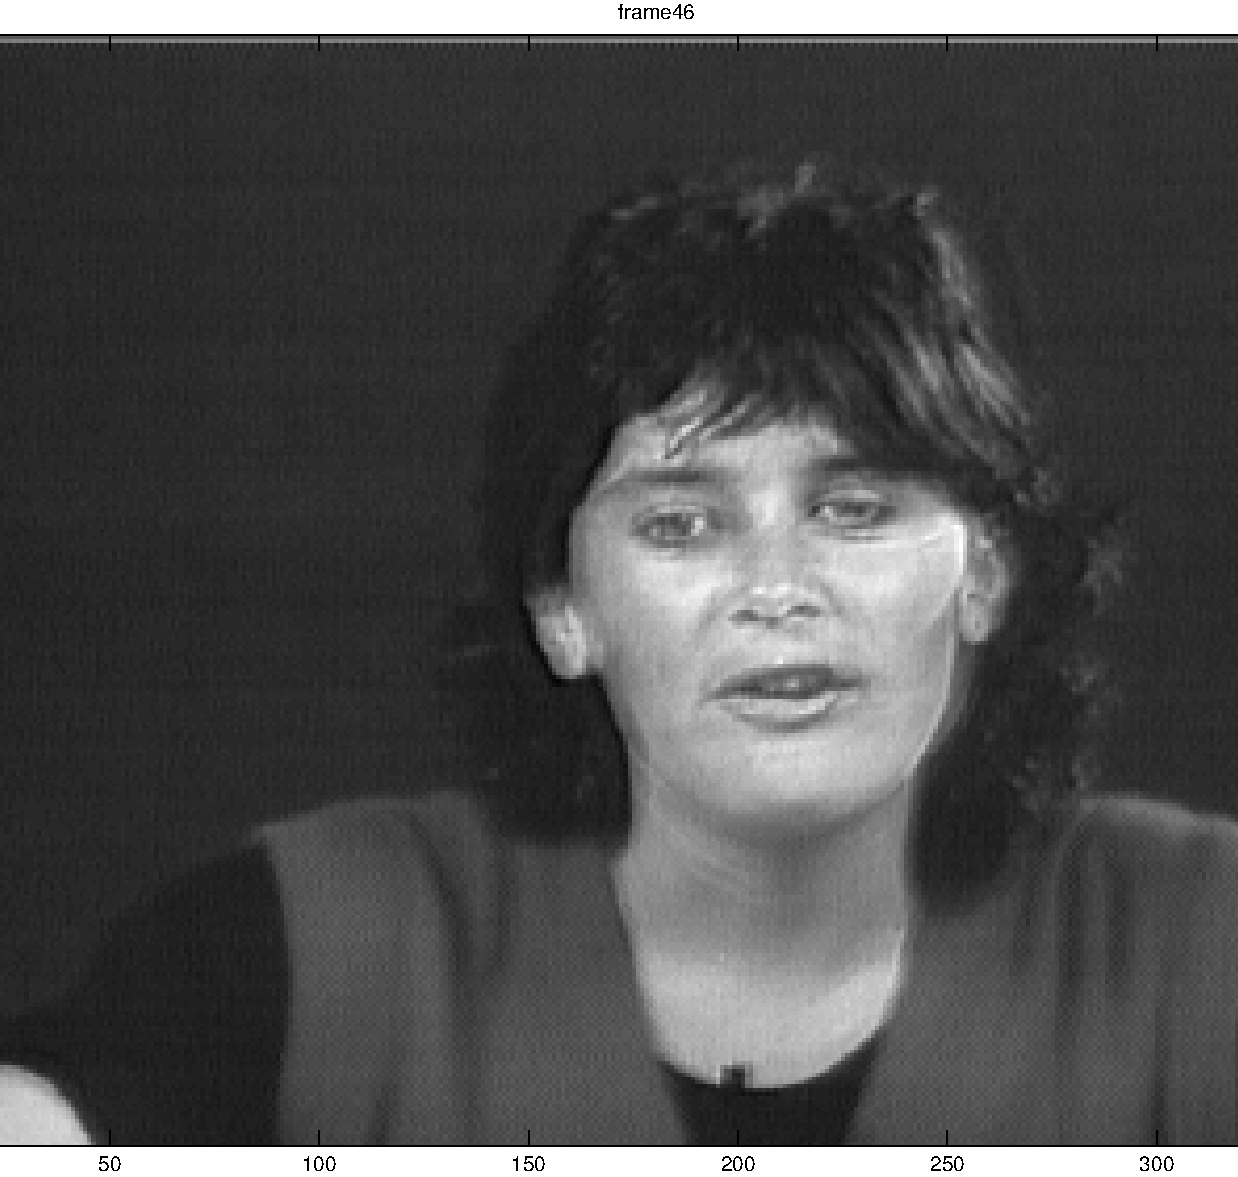
\includegraphics[width=0.24\textwidth]{../diagrams/missaGpdsframe46.pdf}
	\label{fig:missa1}
}
\subfigure[]{
	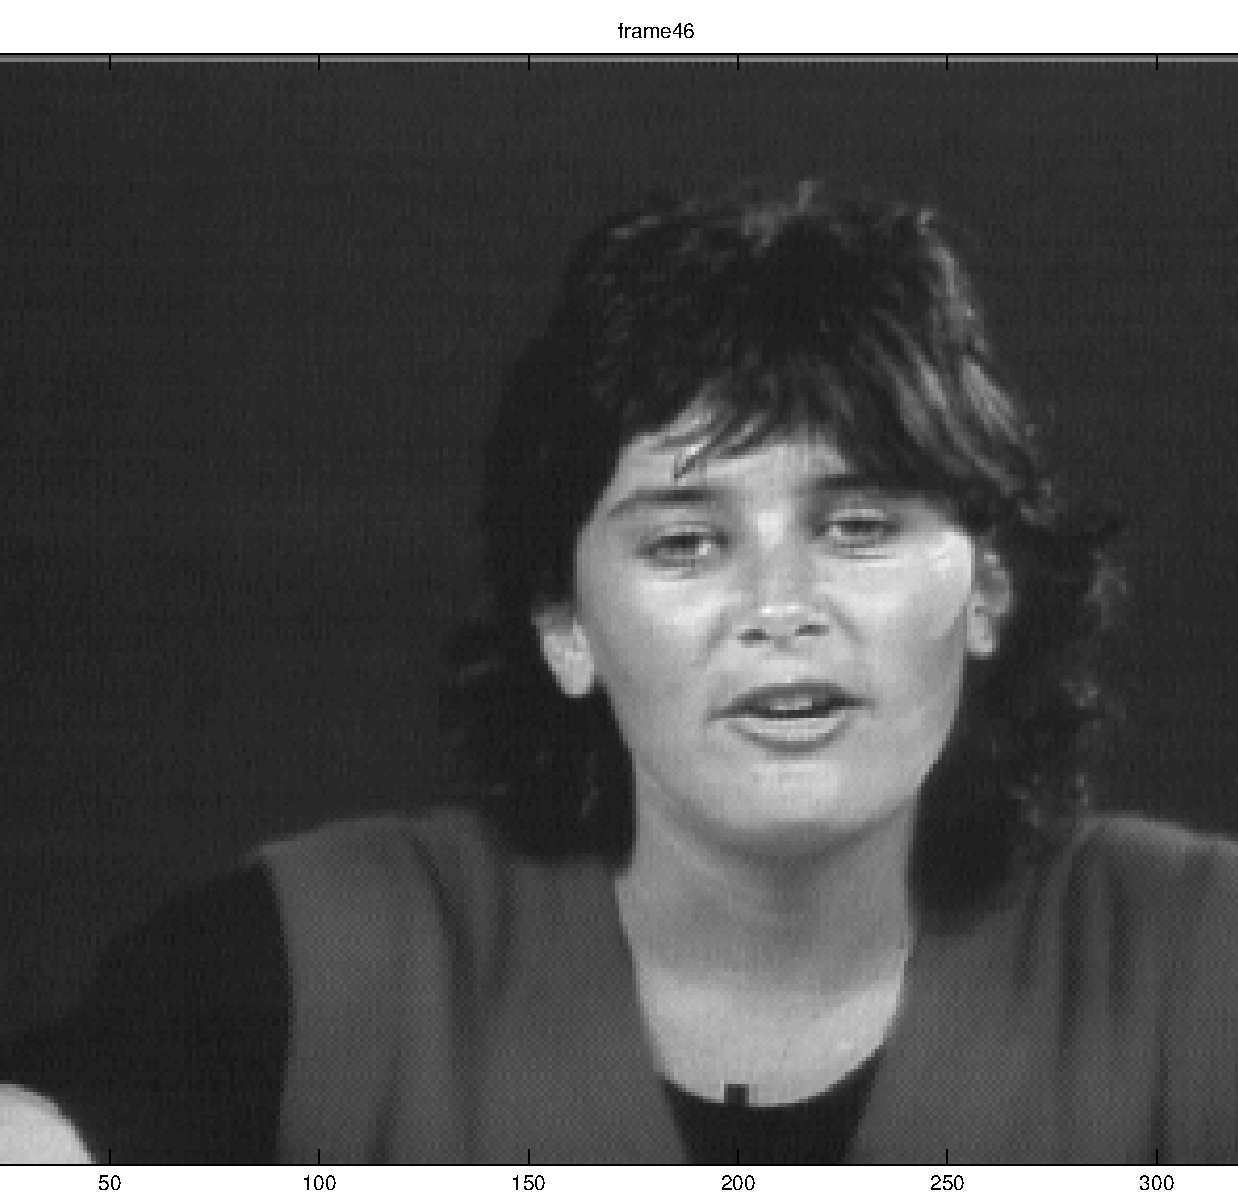
\includegraphics[width=0.24\textwidth]{../diagrams/missaYtsOrigframe46.pdf}
	\label{fig:missa2}
}
\subfigure[]{
	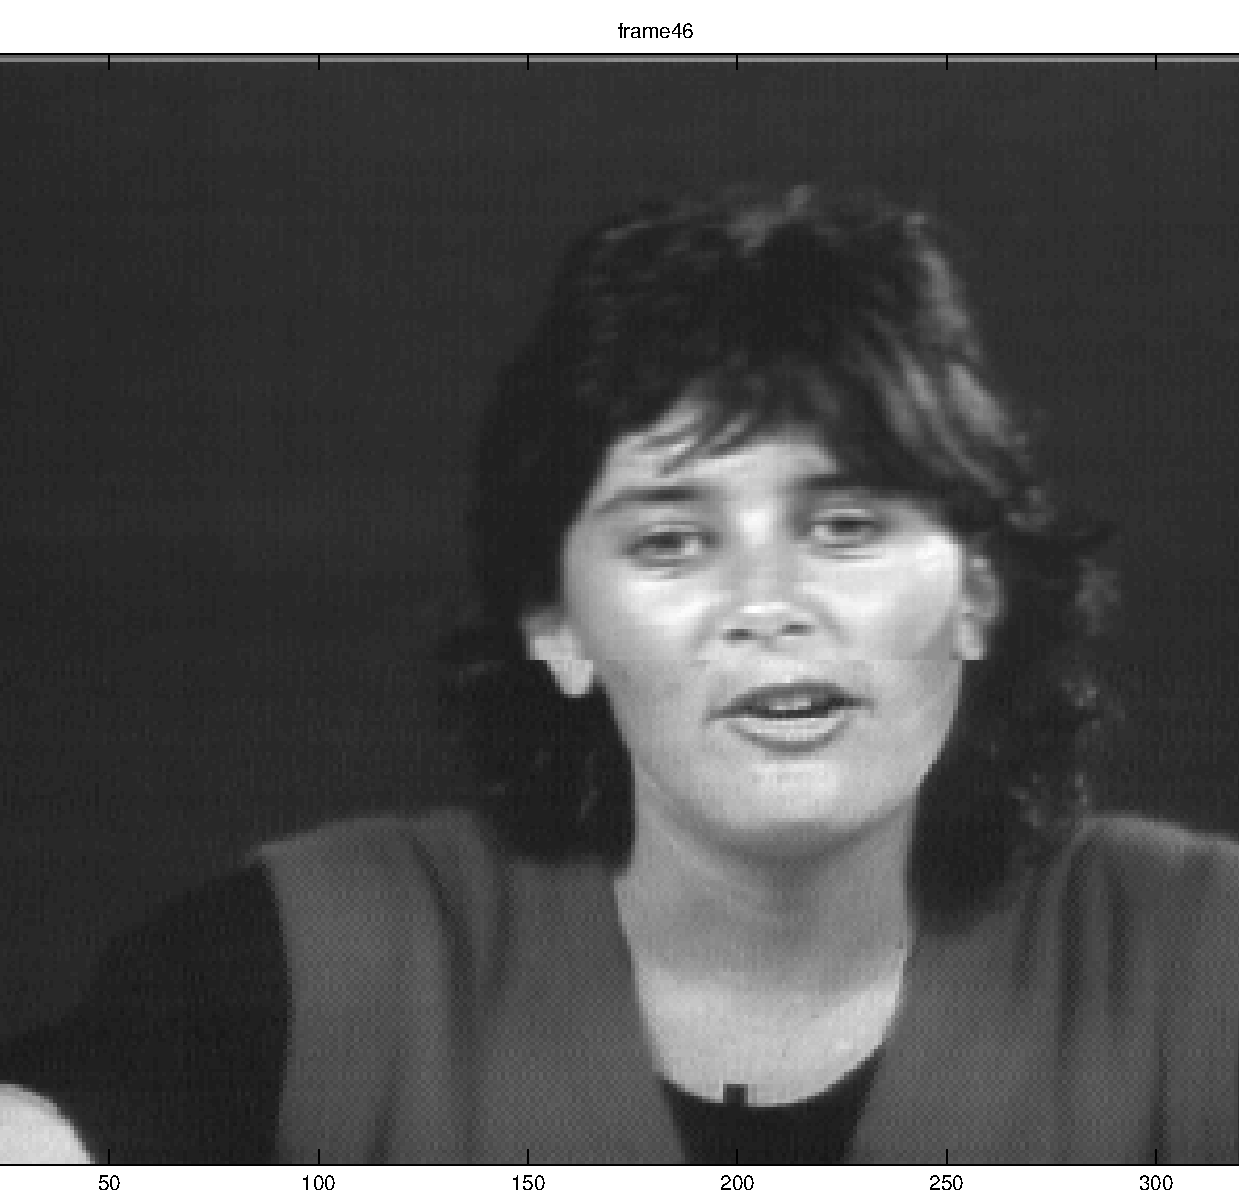
\includegraphics[width=0.24\textwidth]{../diagrams/missaNNframe46}
	\label{fig:missa3}
}
\subfigure[]{
	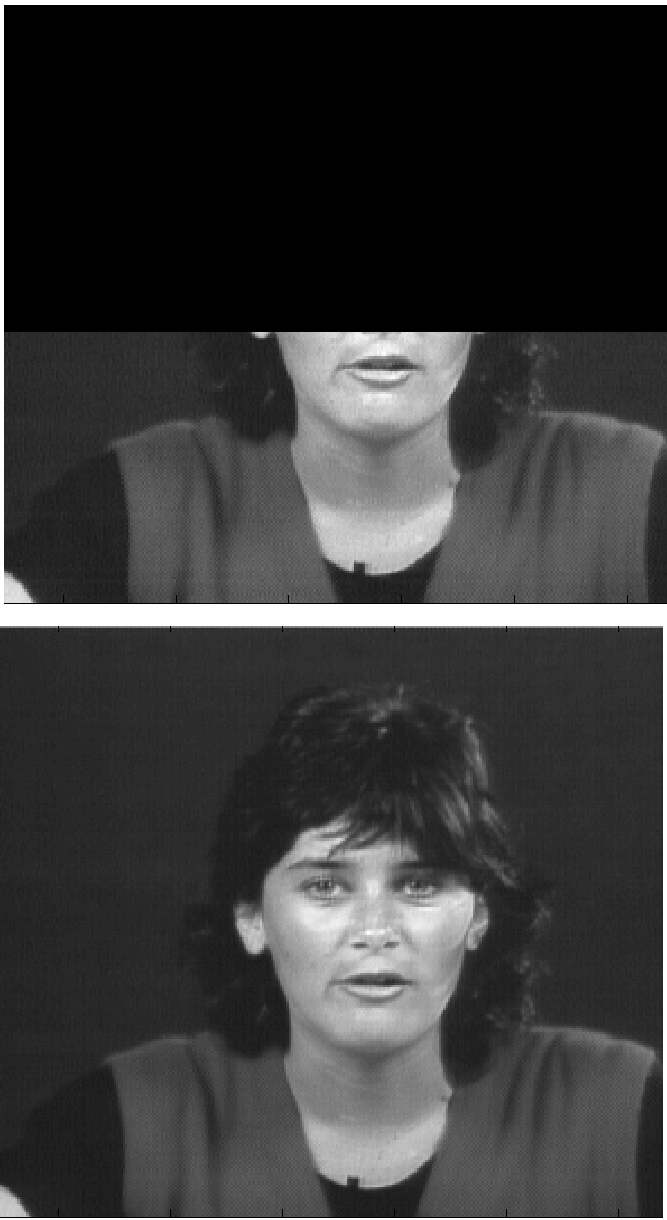
\includegraphics[width=0.12\textwidth]{../diagrams/missaGpdsPredFrame17}
	\label{fig:missa4}
}
\subfigure[]{
	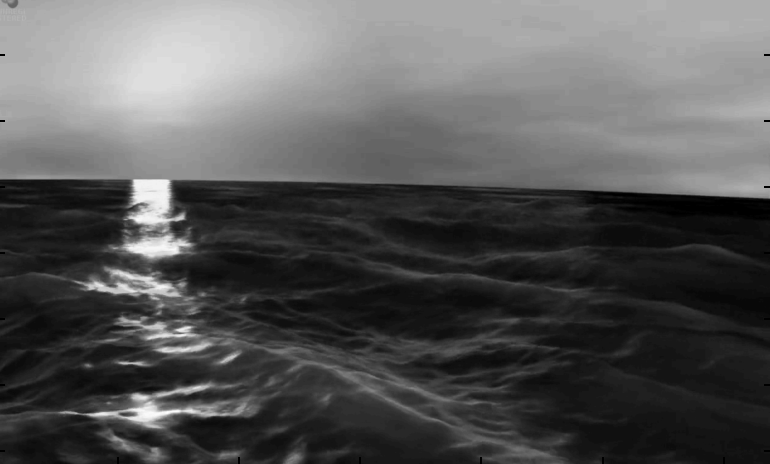
\includegraphics[width=0.39\textwidth]{../diagrams/ocean25_VGPDS}
	\label{fig:ocean1}
}
%\subfigure[]{
%	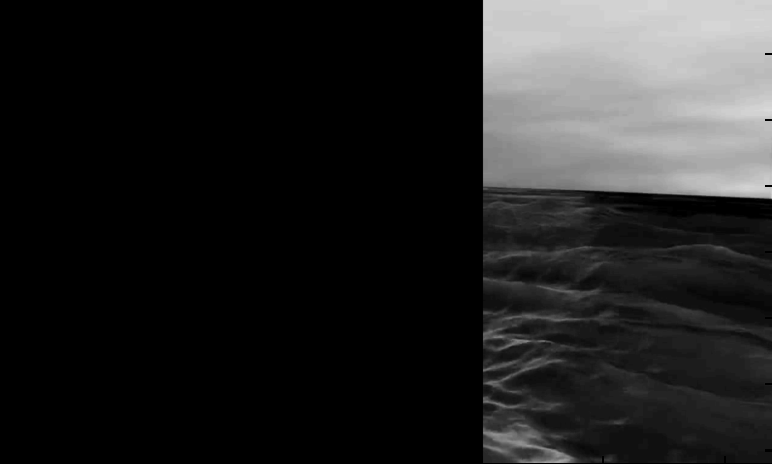
\includegraphics[width=0.28\textwidth]{../diagrams/ocean25_Yts}
%	\label{fig:ocean2}
%}
\subfigure[]{
	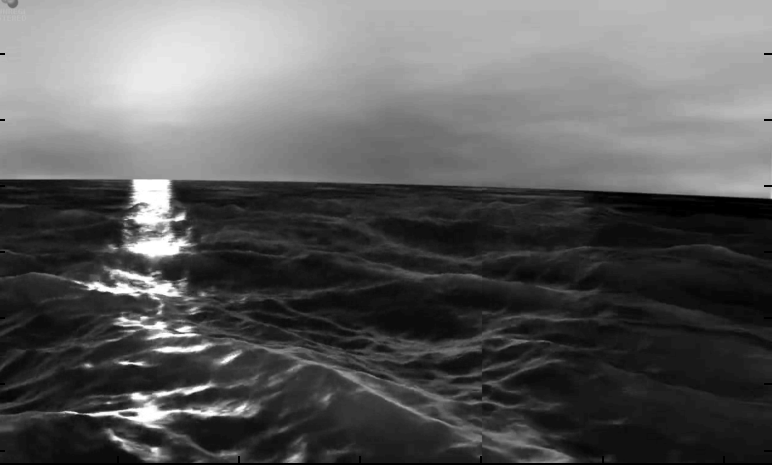
\includegraphics[width=0.39\textwidth]{../diagrams/ocean25_NN}
	\label{fig:ocean3}
}
\subfigure[]{
	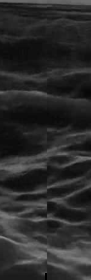
\includegraphics[width=0.08\textwidth]{../diagrams/ocean25_NN_closeup}
	\label{fig:ocean4}
}
      

\end{center}
\caption{\small{
    \subref{fig:missa1} and \subref{fig:missa3} demonstrate the reconstruction achieved by Dyn. VGPLVM and NN respectively for one of the most challenging frames \subref{fig:missa2} of the `missa' video, i.e.\ when translation occurs. \subref{fig:missa4} shows another example of the reconstruction achieved by Dyn. VGPLVM given the partially observed image. \subref{fig:ocean1} (Dyn. VGPLVM) and \subref{fig:ocean3} (NN) depict the reconstruction achieved for a frame of the `ocean' dataset. %, given the partial information shown in figure \subref{fig:ocean2}.
Notice that in both of the aforementioned datasets, our method recovers a smooth image, in contrast to the simple NN (a close up of this problem with NN for the `ocean' video is shown in figure \subref{fig:ocean4}). In contrast to the NN method, which works in the whole high dimensional pixel space, VGPLVM reconstructed the images using a $12$ and a $9$-dimensional compression for the `missa' and the `ocean' video respectively.
}
}
\label{fig:video1}
\end{figure}
As can be seen in figure \ref{fig:video1}, the Dynamical Variational GP-LVM predicts pixels which
are smoothly connected with the observed part of the image, whereas the NN method cannot fit the predicted pixels in the overall context.
This problem with NN is shown in figure \ref{fig:video1}\subref{fig:ocean4}, but it can be seen more evidently in the corresponding video files.

\begin{figure}[ht]
\begin{center}
%\subfigure[]{
%	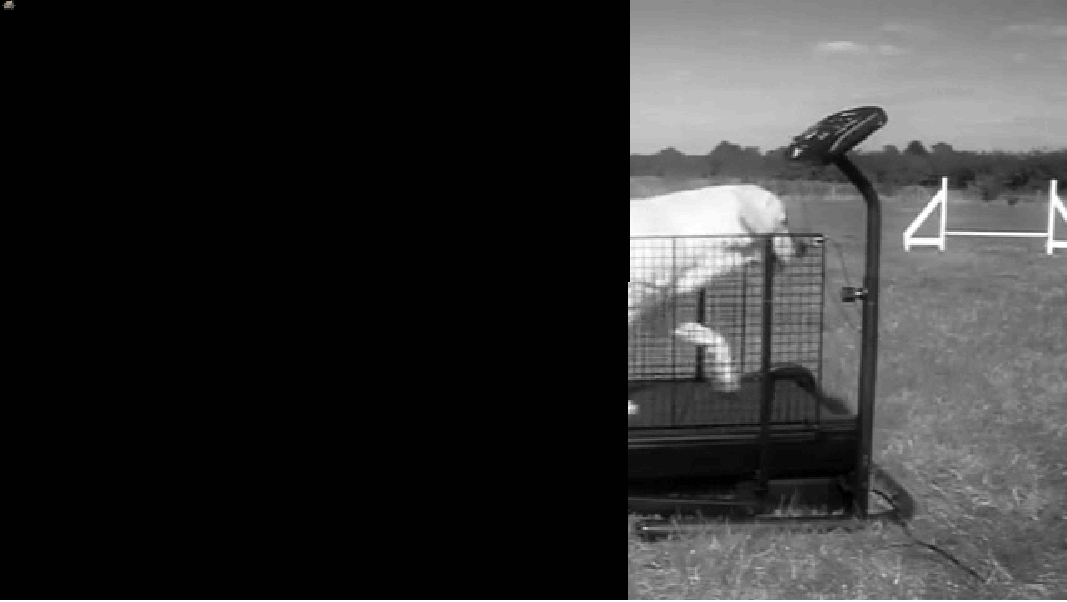
\includegraphics[width=0.23\textwidth]{../diagrams/supplDogPredYts5}
%	\label{fig:suppDog1}
%}
%\subfigure[]{
%	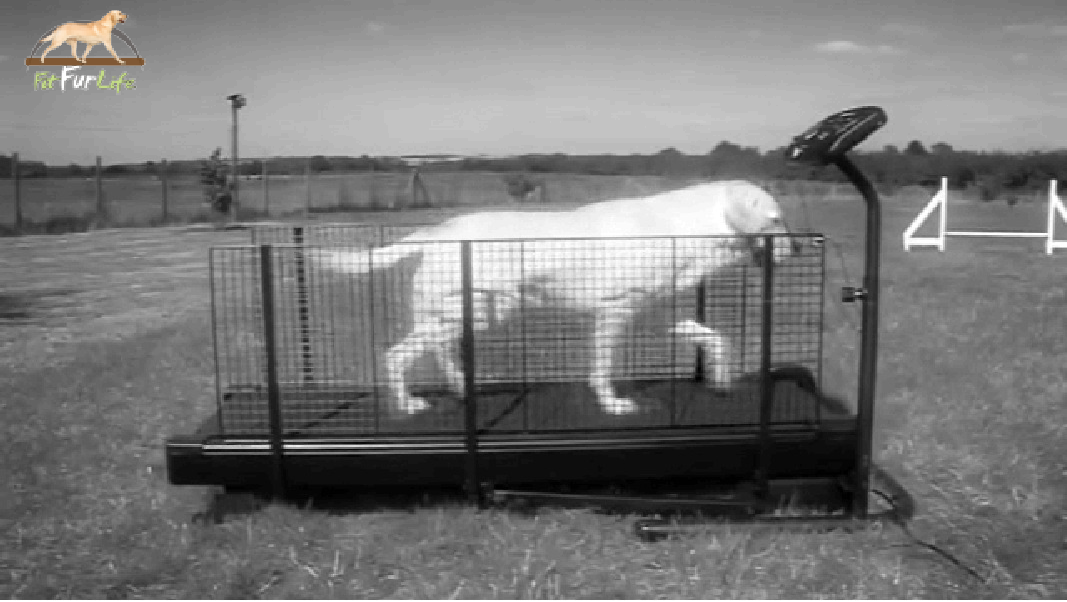
\includegraphics[width=0.23\textwidth]{../diagrams/supplDogPredGpds5}
%	\label{fig:suppDog2}
%}
\subfigure[]{
	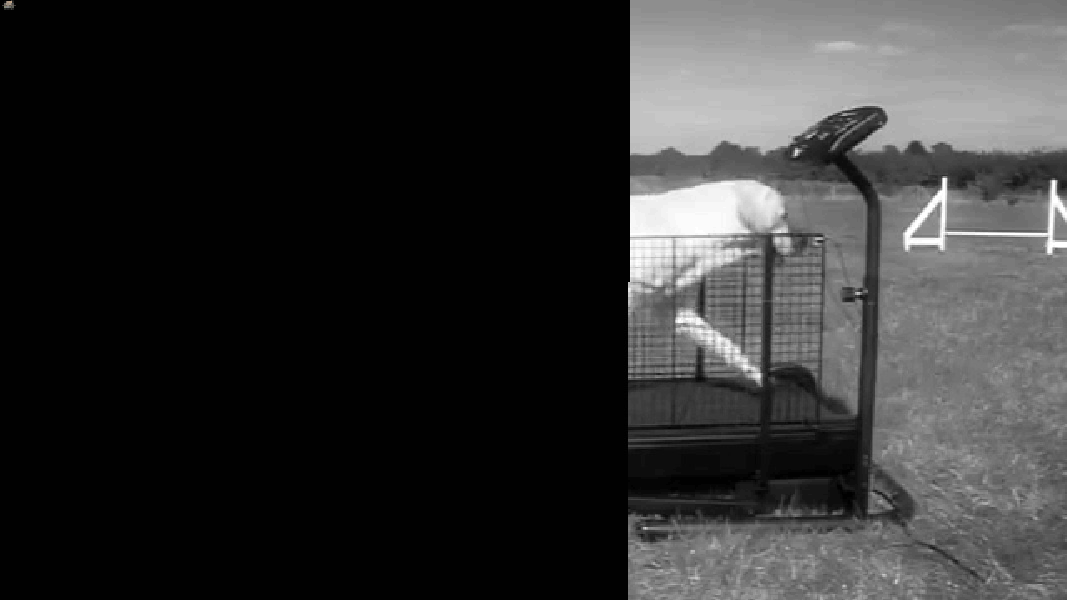
\includegraphics[width=0.23\textwidth]{../diagrams/dogPredYts6}
	\label{fig:dog3}
}
\subfigure[]{
	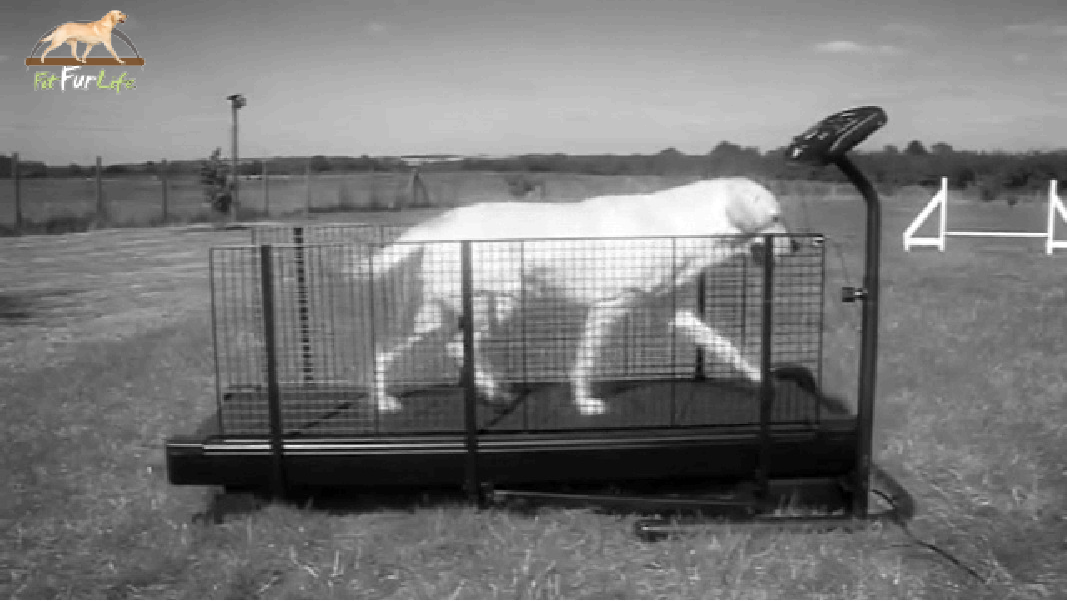
\includegraphics[width=0.23\textwidth]{../diagrams/dogPredGpds6}
	\label{fig:dog4}
}
\subfigure[]{
	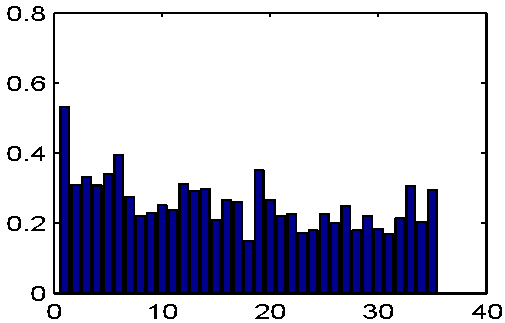
\includegraphics[width=0.23\textwidth]{../diagrams/dog_scalesInit}
	\label{fig:scalesDogInit}
}
\subfigure[]{
	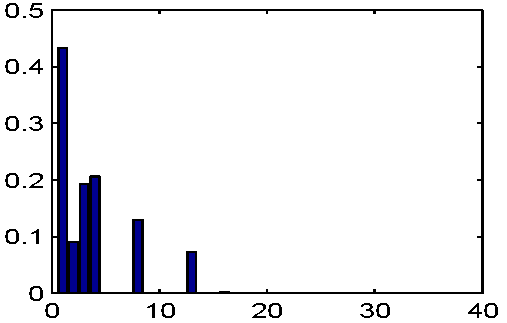
\includegraphics[width=0.23\textwidth]{../diagrams/dog_scalesOpt}
	\label{fig:scalesDogOpt}
}      
\end{center}
\caption{\small{
 An example for the reconstruction achieved for the `dog' dataset. $40\%$ of the test image's pixels (figures \subref{fig:dog3}  were presented  to the model, which was able to successfully reconstruct them, as can be seen in \subref{fig:dog4}.     
Here, we also demonstrate the ability of the model to automatically select the latent dimensionality by showing the initial lengthscales (fig: \subref{fig:scalesDogInit}) of the ARD covariance function and the values obtained after training (fig: \subref{fig:scalesDogOpt}) on the `dog' data set.
}
}
\label{fig:dogRec}
\end{figure}

%\highlight{TODO:} Show what the Latent space represents (maybe can create video from sampling along each of the retained dimensions).

\par As a second task, we used our generative model to create new
samples and generate a new video sequence. This is most effective for
the `dog' video as the training examples were approximately periodic
in nature. The model was trained on 60 frames (time-stamps $[t_1,
t_{60}]$) and we generated new frames which correspond to the next
40 time points in the future. The only input given for this generation
of future frames was the time-stamp vector, $[t_{61}, t_{100}]$. The
results show a smooth transition from training to test and amongst the
test video frames. The resulting video of the dog continuing to run is
sharp and high quality. This experiment demonstrates the ability of
the model to reconstruct massively high dimensional images without
blurring. Frames from the result are shown in figure
\ref{fig:dog}. The full video is available in the supplementary
material.


\begin{figure}[ht]
\begin{center}
\subfigure[]{
	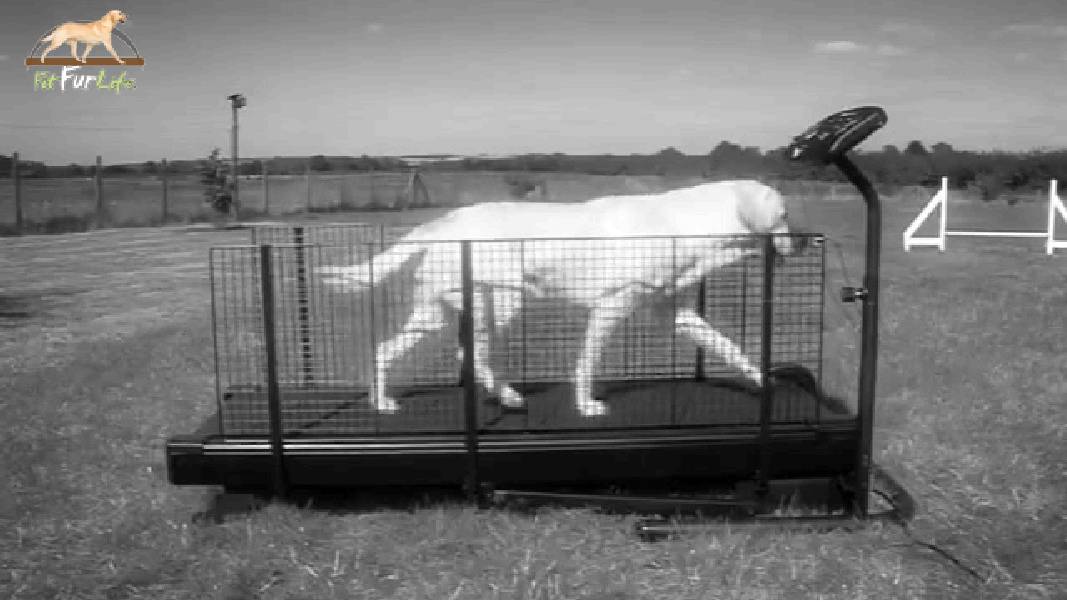
\includegraphics[width=0.23\textwidth]{../diagrams/dogGeneration_lastOfTraining}
	\label{fig:dogTrain}
}
\subfigure[]{
	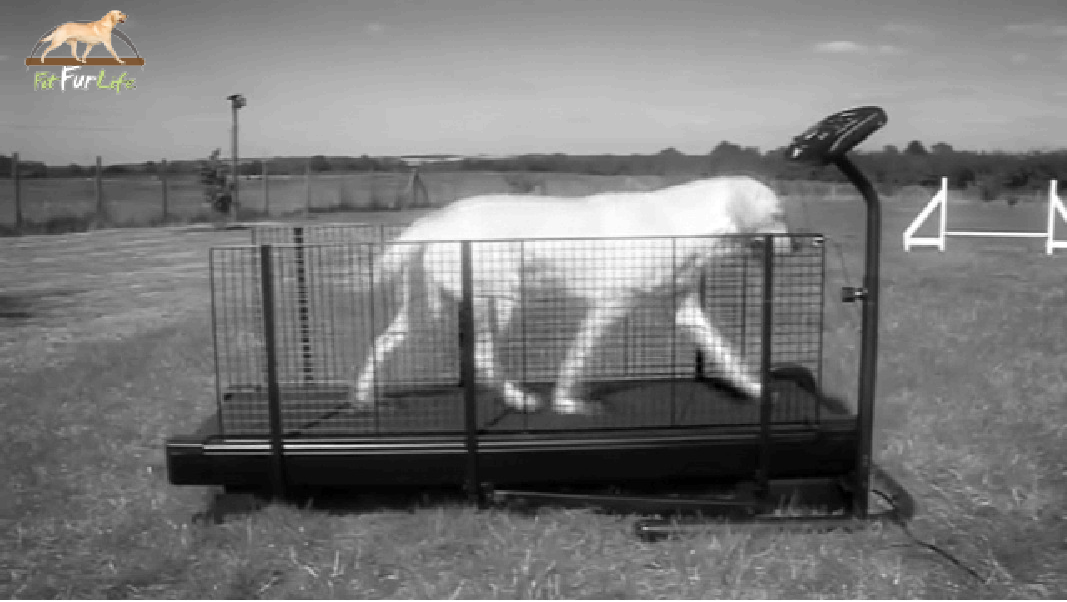
\includegraphics[width=0.23\textwidth]{../diagrams/dogGeneration_firstOfTest}
	\label{fig:dogTest1}
}
\subfigure[]{
	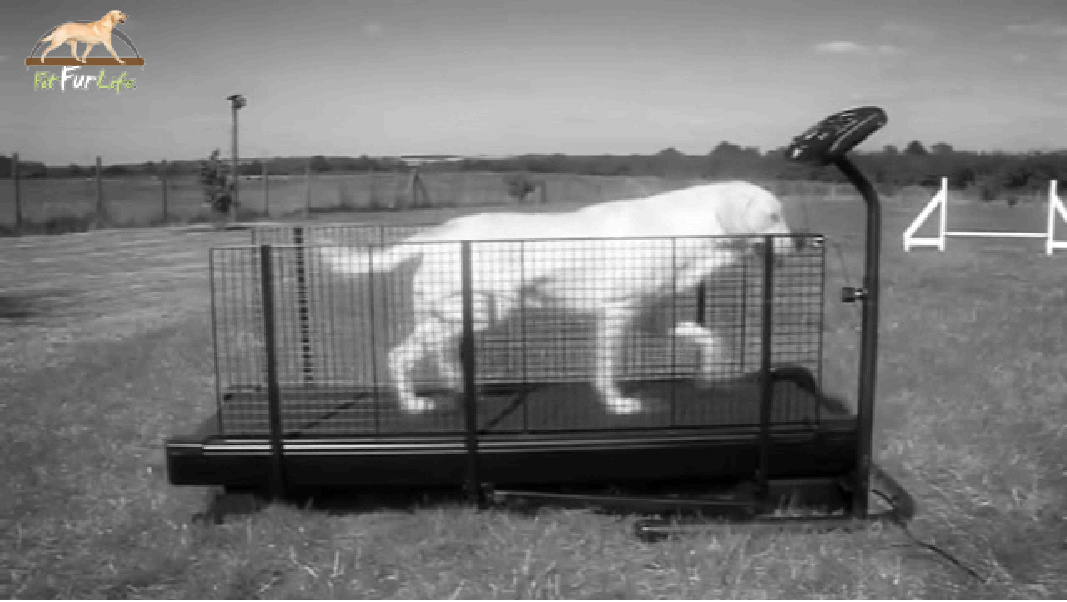
\includegraphics[width=0.23\textwidth]{../diagrams/dogGeneration_frame14}
	\label{fig:dogTest2}
}
\end{center}
\caption{ \small{
The last frame of the training video \subref{fig:dogTrain} is smoothly followed by the first frame \subref{fig:dogTest1} of the generated video. A subsequent generated frame can be seen in \subref{fig:dogTest2}}.}
\label{fig:dog}
\end{figure}






%----------------------------------------------- CONCLUSION -----------------------------------------------
\section{\label{section:conclusion} Conclusion}

We have introduced an approximation to the marginal likelihood of the Gaussian process latent variable model
in the form of a variational lower bound. This provides a Bayesian training procedure which is robust
to overfitting and allows for the appropriate dimensionality of the latent space to be automatically determined.
Our framework is extended for the case where the observed data consitute multivariate timeseries and,
therefore, we obtain a very generic method for dynamical systems modelling able to capture complex, non-linear
correlations. We demonstrated the advantages of the rigorous lower bound defined in our framework on a range of
disparate real world data sets. This also emphasised the ability of the model to handle vast dimensionalities.

\par Our approach can immediately be applied to training Gaussian processes with uncertain inputs where these
inputs have Gaussian prior densities. We also envisage several other extensions that become computationally
feasible using the same set of methodologies we espouse. Latent space priors other than the
temporal Gaussian process used here, would result in non-linear dynamical models with different properties. In
particular, a Kalman filter or an auto-regressive Gaussian process \cite{GPDM} can be considered.
Further, being able to select the latent space dimensionality automatically makes future hierarchical
or mixture Bayesian modelling approaches seem promising. This is because the key difficulty with the
GP-LVM based methods
considered so far (\eg \cite{hgplvm, Salzmann:2010vh}) is that the dimensionality of the latent
space for each level of the hierarchy or for
each element of the mixture must be set by hand or with ad-hoc techniques, something which is clearly
suboptimal and inefficient.



%----------------------------------------------- ACKNOWLEDMENTS -----------------------------------------
\subsubsection*{Acknowledgments}
Research was partially supported by the University of Sheffield Moody endowment fund and the Greek State
 Scholarships Foundation (IKY).
We also thank Colin Litster and ``Fit Fur Life'' for allowing us to use their video files as datasets.

%\bibliographystyle{apalike}
\bibliographystyle{ieeetr}
\renewcommand*{\refname}{\begin{normalsize}References\end{normalsize}}
\bibliography{vargplvm,lawrence,other,zbooks}
%\singlespace
%\bibliography{paper}







\newpage
 \begin{center}
 \begin{Large}
 \textbf{
% Gaussian Process Dynamical Systems\\
 Appendix
 } \\
 \end{Large}
% \noindent \newline
% \textbf{Andreas Damianou, Michalis Titsias, Neil Lawrence}
 \end{center}
\appendix







\section{Calculating $\hat{\mathcal{F}_d}(q, \boldsymbol \theta)$}

We have:
\begin{equation}
\hat{\mathcal{F}_d} \geq
	\log \int e^{\la \log N \left( \bfy_d | \bfa_d, \beta^{-1} I_d \right) \ra_{q(X)}}
		p(\bfu_d) \intd \bfu_d -\mathcal{A} .
\end{equation}

with:

\begin{equation}
\label{boundFIntegral}
\int e^{\la \log N \left( \bfy_d | \bfa_d, \beta^{-1} I_d \right) \ra_{q(X)}}
		p(\bfu_d) d\bfu_d = 
\int e^{\la \log N \left( \bfy_d | \bfa_d, \beta^{-1} I_d \right) \ra_{q(X)} + \log p(\bfu_d)}
		d\bfu_d
\end{equation}

The expectation involved in the quantity above is calculated as:
\begin{align}
\la \log N \left( \bfy_d | \bfa_d, \beta^{-1} I_d \right) \ra_{q(X)} = {}& 
- \frac{N}{2} \log (2 \pi) - \frac{1}{2} \log \vert \beta^{-1} I_d \vert 
- \frac{1}{2} Tr \la \beta I_d \left( \bfy_d - \bfa_d) (\bfy_d - \bfa_d \right)^\T \ra \nonumber \\
={}&
- \frac{N}{2} \log ( 2 \pi ) - \frac{1}{2} \log \vert \beta^{-1} I_d \vert 
- \frac{1}{2} Tr \left[ \beta I_d \left( \bfy_d \bfy_d^\T - 
2 \bfy_d \la \bfa_d^\T \ra + \la \bfa_d \bfa_d^\T \ra \right) \right] \label{boundFExpectation1}
\end{align}

but $\la \bfa_d \ra = \la K_{NM} \ra K_{MM}^{-1} \bfu_d$ and 
$\la \bfa_d \bfa_d^\T \ra = \la K_{NM} \ra K_{MM}^{-1} \bfu_d \bfu_d^\T K_{MM}^{-1} \la K_{NM}^\T \ra$ ($K_{MM}$ is symmetric so it's equal to its transpose), so \eqref{boundFExpectation1} now becomes:
\begin{align}
\la \log N \left( \bfy_d | \bfa_d, \beta^{-1} I_d \right) \ra_{q(X)} = {}&
- \frac{N}{2} \log (2 \pi) - \frac{1}{2} \log \vert \beta^{-1} I_d \vert \nonumber \\
{}& - \frac{1}{2} Tr \left[
	\beta I_d \left( \bfy_d \bfy_d^\T - 2 \bfy_d \bfu_d^\T K_{MM}^{-1} \la K_{NM}^\T \ra + 
	\bfu_d^\T K_{MM}^{-1} \la K_{NM}^\T K_{NM} \ra K_{MM}^{-1} \bfu_d \right) \right]
\end{align}

We now set:
\begin{equation*}
\Psi_0 = Tr(\langle \mathit{K_{NN}} \rangle_{q(\mathit{X})}) \;, \;\;
\Psi_1 = \langle \mathit{K_{NM}} \rangle_{q(\mathit{X})} \;, \;\;
\Psi_2 = \langle \mathit{K_{MN}} \mathit{K_{NM}} \rangle_{q(\mathit{X})}
\end{equation*}

and we get:

\begin{align}
{}& \la \log N \left( \bfy_d | \bfa_d, \beta^{-1} I_d \right) \ra_{q(X)} = \nonumber \\
{}& \;\;\;\;\;\;
	 - \frac{N}{2} \log (2 \pi) - \frac{1}{2} \log \vert \beta^{-1} I_d \vert \nonumber \\
{}& \;\;\;\;\;\; 
	- \frac{1}{2} Tr \left[
	\beta I_d \left( \bfy_d \bfy_d^\T - 2 \bfy_d \bfu_d^\T K_{MM}^{-1} \Psi_1^\T + 
	\bfu_d^\T K_{MM}^{-1} \Psi_2 K_{MM}^{-1} \bfu_d \right) \right]
\end{align}

We now add $\log p(\bfu_d)$ so as to get the full quantity which is integrated in \eqref{boundFIntegral}. Thus, we use \eqref{priorF2} and we get:

\begin{align}
{}& \la \log N \left( \bfy_d | \bfa_d, \beta^{-1} I_d \right) \ra_{q(X)} + \log p(\bfu_d) = \nonumber \\
{}& \;\;\;\;\;\;
	 - \frac{N}{2} \log (2 \pi) - \frac{1}{2} \log \vert \beta^{-1} I_d \vert \nonumber \\
{}& \;\;\;\;\;\; 
	- \frac{1}{2} Tr \left[
	\beta I_d \left( \bfy_d \bfy_d^\T - 2 \bfy_d \bfu_d^\T K_{MM}^{-1} \Psi_1^\T + 
	\bfu_d^\T K_{MM}^{-1} \Psi_2 K_{MM}^{-1} \bfu_d \right) \right] \nonumber \\
{}& \;\;\;\;\;\;
	- \frac{M}{2} \log (2 \pi ) - \frac{1}{2} \log \vert K_{MM} \vert - 
	\frac{1}{2} Tr \left( K_{MM}^{-1} \bfu_d \bfu_d^\T \right)  \label{boundFIntegral2}
\end{align}

By completing the square, \eqref{boundFIntegral2} can be rewritten as:
\begin{align}
{}& \la \log N \left( \bfy_d | \bfa_d, \beta^{-1} I_d \right) \ra_{q(X)} + \log p(\bfu_d) = \nonumber \\
{}& \;\;\;\;\;\;
  - \frac{N}{2} \log (2 \pi) - \frac{1}{2} \log \vert \beta^{-1} I_d \vert
  - \frac{1}{2} \log \vert K_{MM} \vert \nonumber \\
 {}& \;\;\;\;\;\;
  - \frac{\beta}{2} \bfy_d^\T \bfy_d + \frac{1}{2} m^\T S^{-1} m + \frac{1}{2} \log \vert S \vert
  + \log N(\bfu_d | m, S) \label{boundFIntegral3}
\end{align}
where
\begin{align}
S = {}& \left( \beta K_{MM}^{-1} \Psi_2 K_{MM}^{-1} + K_{MM}^{-1} \right)^{-1} \label{boundFVarS} \mbox{\;\;\;\; and} \\
m = {}& \beta S K_{MM}^{-1} \Psi_1^\T \bfy_d \label{boundFVarm}
\end{align}

We can now obtain the final expression for \eqref{boundFIntegral} by simply putting the quantity of \eqref{boundFIntegral3} on the exponent and integrating. By doing so, we get:

\begin{align}
{}& \int e^{\la \log N \left( \bfy_d | \bfa_d, \beta^{-1} I_d \right) \ra_{q(X)}}
		p(\bfu_d) d\bfu_d = \nonumber \\
= {}& \;\;\;\;
\int
 exp \left(
\underbrace{
  - \frac{N}{2} \log (2 \pi) - \frac{1}{2} \log \vert \beta^{-1} I_d \vert
  - \frac{1}{2} \log \vert K_{MM} \vert
  - \frac{\beta}{2} \bfy_d^\T \bfy_d + \frac{1}{2} m^\T S^{-1} m + \frac{1}{2} \log \vert S \vert
}_{B}
 \right)  \nonumber \\
{}& \;\;\;\;\;\;
\;\;  exp \left( \log N(\bfu_d | m, S) \right) d\bfu_d \nonumber \\
= {}& \;\;\;\;
	e^{B} \int e^{\log N(\bfu_d | m, S)} d\bfu_d = e^{B} \nonumber \\
= {}& \;\;\;\;
	(2 \pi)^{-\frac{N}{2}} \beta^{\frac{N}{2}} \vert K_{MM} \vert^{-\frac{1}{2}}
	e^{- \frac{\beta}{2} \bfy_d^\T \bfy_d} \vert S \vert^{\frac{1}{2}} e^{\frac{1}{2}m^\T S^{-1} m} \nonumber
\end{align}

We now replace the first occurrence of $S$ with its equal (from \eqref{boundFVarS}) and we get:
\begin{align}
{}& \int e^{\la \log N \left( \bfy_d | \bfa_d, \beta^{-1} I_d \right) \ra_{q(X)}}
		p(\bfu_d) d\bfu_d = \nonumber \\
= {}& \;\;\;\;
\frac{\beta^{\frac{N}{2}} \vert K_{MM} \vert^{-\frac{1}{2}}}{(2 \pi)^{N/2}} e^{-\frac{\beta}{2} \bfy_d^\T \bfy_d}
	\vert \beta K_{MM}^{-1} \Psi_2 K_{MM}^{-1} + K_{MM}^{-1} \vert^{-\frac{1}{2}} e^{\frac{1}{2} m^\T S^{-1} m} \nonumber \\
= {}& \;\;\;\;
\frac{\beta^{\frac{N}{2}} \vert K_{MM} \vert^{-\frac{1}{2}} \vert K_{MM} \vert e^{-\frac{\beta}{2} \bfy_d^\T \bfy_d}}
	 {(2 \pi)^{N/2}  \vert \beta \Psi_2 + K_{MM} \vert^{\frac{1}{2}} }
	 e^{\frac{1}{2} \bfy_d^\T W' \bfy_d}
\label{boundFIntegralFinal2}
\end{align}
with $W' = \beta^2 \Psi_1 (\beta \Psi_2 + K_{MM})^{-1} \Psi_1^\T$.
Finally, we perform some further calculations in \eqref{boundFIntegralFinal2} and replace in \eqref{boundFAnalyticallyFinalIntegral} (also replacing the quantity $A$ with its equal); we thus have the final form of the likelihood part of the lower bound:
%%%

\begin{equation}
\label{FdFinal}
\mathit{\tilde{F}_d}(q, \boldsymbol \theta) \geq \log \left[ 
	\frac{(\beta)^{\frac{N}{2}} \vert \mathit{K_{MM}} \vert ^\frac{1}{2} }
		 {(2\pi)^{\frac{N}{2}} \vert \beta \Psi_2 + \mathit{K_{MM}}  \vert ^\frac{1}{2} } 
	 e^{-\frac{1}{2} \mathbf{y}^{T}_{d} W \mathbf{y}_d}
	 \right]	 -
	 \frac{\beta \psi_0}{2} + \frac{\beta}{2} 
	 Tr \left( \mathit{K_{MM}^{-1}} \Psi_2 \right)	
\end{equation}

\noindent where:
\begin{equation}
\label{psis}
\Psi_0 = Tr(\langle \mathit{K_{NN}} \rangle_{q(\mathit{X})}) \;, \;\;
\Psi_1 = \langle \mathit{K_{NM}} \rangle_{q(\mathit{X})} \;, \;\;
\Psi_2 = \langle \mathit{K_{MN}} \mathit{K_{NM}} \rangle_{q(\mathit{X})}
\end{equation}

\noindent and $W = \beta I_N - \beta^2 \Psi_1 (\beta \Psi_2 + K_{MM})^{-1} \Psi_1^T$. \newline

\par Note that \textbf{$\Psi_2$ is a symmetric matrix}, since it's an average of the multiplication of a matrix with its transpose: $K_{MN} K_{NM} = K_{MN} K_{MN}^T$.
$\Psi$s can be computed analytically as described in \cite{BayesianGPLVM}. 

Then, the complete expression for $\tilde{F}(q, \boldsymbol \theta)$ is obtained by summation over $d$:
\begin{align}
\tilde{F}(q, \boldsymbol \theta) &{} = \sum_{d=1}^D \tilde{F}_d(q, \boldsymbol \theta) \nonumber \\
   &{} = \log \left[ 
	\frac{(\beta)^{\frac{ND}{2}} \vert \mathit{K_{MM}} \vert ^\frac{D}{2} }
		 {(2\pi)^{\frac{ND}{2}} \vert \beta \Psi_2 + \mathit{K_{MM}}  \vert ^\frac{D}{2} } 
	 e^{-\frac{1}{2} \sum_{d=1}^D \mathbf{y}^{T}_{d} W \mathbf{y}_d}
	 \right]	 -
	 \frac{\beta D \psi_0}{2} + \frac{\beta D}{2} 
	 Tr \left( \mathit{K_{MM}^{-1}} \Psi_2 \right)	 \label{FFinal}
\end{align}






%-------------------------
\section{Calculating the $\Psi$ quantities}
To obtain an explicit evaluation of the variational lower bound we
need to compute the statistics $(\psi_0,\Psi_1,\Psi_2)$. We can
rewrite the $\psi_0$ statistic as $\psi_0 = \sum_{n=1}^N \psi_0^n$
where
\begin{equation}
\psi_0^n = \int k(\bfx_n,\bfx_n) \mathcal{N}(\bfx_n |\bfmu_n , S_n) d \bfx_n.
\label{eq:psi0}
\end{equation}
Here, $S_n$ is a vector $\{ S_{n,q}\}_{q=1}^Q$ and constitutes a diagonal
covariance matrix. This matrix is diagonal since the GP-LVM likelihood is
fully factorised, given $f$, something which is obvious from \eqref{generative}.
%
$\Psi_1$ is an $N \times M$ matrix such that  
\begin{equation}
  (\Psi_1)_{nm} = \int k(\bfx_n,\bfzi_m) \mathcal{N}(\bfx_n|\bfmu_n, S_n) d
  \bfx_n.
\label{eq:psi1}
\end{equation}
$\Psi_2$ is an $M \times M$ matrix which is written as
 $\Psi_2 = \sum_{n=1}^N \Psi_2^n$ where $\Psi_2^n$ is such that 
\begin{equation}
  (\Psi^n_2)_{m m'} = \int k(\bfx_n,\bfzi_m)
  k(\bfzi_{m'},\bfx_n) \mathcal{N}(\bfx_n|\bfmu_n, S_n) d \bfx_n.
\label{eq:psi2}
\end{equation}
The above computations involve convolutions of the covariance function
with a Gaussian density. For some standard kernels such the ARD
squared exponential (SE) covariance and the linear covariance function
these statistics are obtained analytically. In particular for the ARD
SE kernel, $\psi_0 = N \sigma_f^2$,
$$
(\Psi_1)_{nm} = \sigma^2_f \prod_{q=1}^Q
\frac{ e^{ - \frac{1}{2} \frac{ \alpha_q (\bfmu_{nq}  -
    \bfzi_{mq})^2}{\alpha_q S_{nq} + 1}}}
{( \alpha_q S_{nq} + 1)^{\frac{1}{2}}} 
$$ 
and 
$$
(\Psi^n_2)_{m m'} = \sigma_f^4 
\prod_{q=1}^Q \frac{ e^{-  \frac{\alpha_q (z_{mq} -
    z_{m'q})^2}{4} - \frac{\alpha_q \left(\mu_{nq} -
 \bar{z}_{q} \right)^2}{2 \alpha_q S_{nq} + 1}}}
{(2 \alpha_q S_{nq} + 1)^{\frac{1}{2}}},
$$  
where $\bar{z}_{q} = \frac{(z_{mq} + z_{m'q})}{2}$. This gives us all
the components we need to compute the variational lower bound for the
ARD SE kernel. For the linear covariance function the integrals
are also tractable. Suppose the kernel function follows the ARD linear
form:
\begin{equation} 
k(\bfx,\bfx') = \bfx^T A \bfx', 
\end{equation}
where $A$ is a positive definite diagonal covariance matrix.  Learning
the diagonal elements of $A$ will allow to perform automatic model selection of
the dimensionality of the linear latent space in a similar manner to
ARD SE covariance function. Thus, the framework provides an alternative
method to perform Bayesian probabilistic PCA
\cite{Bishop:bayesPCA98,Minka:automatic01}. For this linear kernel
the statistics are such that $ \psi_0^n =
\text{Tr}\left[A (\bfmu_n \bfmu_n^T + S_n) \right]$,
$(\Psi_1)_{nm} = \bfmu_n^T A \bfzi_m$ and $(\Psi_2^n)_{mm'} =
\bfzi_m^T A (\bfmu_n\bfmu_n^T + S_n ) A \bfzi_{m'}$.

Finally, it is worth noticing that the $\Psi$ statistics are computed in 
a decomposable way which is useful when a new data vector % is observed
is inserted into the model. In particular, the statistics 
$\psi_0$ and $\Psi_2$ are written as sums of independent terms
where each term is associated with a data point and similarly 
each column of the matrix $\Psi_1$ is associated with only one data point.
These properties can help to speed up computations during
test time as discussed in section \ref{section:predictions}.  



\section{Derivatives of the variational bound for the dynamical version}
Before giving the expressions for the derivatives of the variational bound \eqref{jensens1},
it should be reminded that the variational parameters $\mu_q$ and $S_q$ (for all $q$s) have been
reparametrised as $S_q = \left( \mathit{K}_t^{-1} + diag(\boldsymbol \lambda_q) \right)^{-1}  \text{ and }   \boldsymbol \mu_q = K_t \bar{\boldsymbol \mu}_q$, where the function $diag(\cdot)$ transforms a vector into a square diagonal matrix and vice versa. Given the above, the set of the parameters to be optimised is 
$( \boldsymbol \theta_f, \boldsymbol \theta_x, \{ \bar{\bfmu}_q, \boldsymbol \lambda_q \}_{q=1}^Q, \tilde{X}$. The gradient w.r.t the inducing points $\tilde{X}$, however, has exactly the same form as for $\boldsymbol \theta_f$ and, therefore, is not presented here. Also notice that from now on we will often use the term ``variational parameters'' to refer to the new quantities $\bar{\bfmu}_q$ and $\boldsymbol \lambda_q$. 

\textbf{Some more notation:} 
\begin{enumerate}
\item $\lambda_q$ is a scalar, an element of the vector $\boldsymbol \lambda_q$ which, in turn, is the main diagonal of the diagonal matrix $\Lambda_q$. 
%\item$\lambda_m \triangleq \boldsymbol \lambda_{q;m}$, i.e. the $m$-th element of the vector $\boldsymbol \lambda_q$ (thus, an instantiation of $\lambda_q$)
\item $S_{ij} \triangleq S_{q;ij}$ the element of $S_q$ found in the $i$-th row and $j$-th column.
\item $\mathbf{s}_q \triangleq \lbrace S_{q;ii} \rbrace_{i=1}^N$, i.e. it is a vector with the diagonal of $S_q$.
%\item $s_i$ is the $i$-th element of $\mathbf{s}_q$.
%\item $diag(\mathbf{s}_q)$ is a matrix full of zeros apart from the main diagonal which contains the vector $\mathbf{s}_q$.
\end{enumerate}

\subsection{Derivatives w.r.t the variational parameters}
\begin{equation}
    \label{derivVarParamSuppl}
\frac{\vartheta \mathcal{F}_v}{\vartheta \bar{\boldsymbol \mu}_q} 
=  K_t \left( \frac{\vartheta \hat{\mathcal{F}}}{\vartheta \boldsymbol \mu_q} - \bar{\boldsymbol \mu}_q \right)
\text{ and }
 \frac{\vartheta \mathcal{F}_v}{\vartheta \boldsymbol \lambda_q}
= - ( S_q \circ S_q) \left( \frac{\vv \hat{\mathcal{F}}}{\vv \mathbf{s}_q} + \frac{1}{2} \boldsymbol \lambda_q \right).
\end{equation}

where:

\begin{align}
 \frac{\hat{\mathcal{F}}(q, \boldsymbol \theta)}{\vartheta \mu_q}
{}& = - \frac{\beta D}{2} \frac{\vartheta \Psi_0}{\vartheta \mu_q}
    + \beta \text{Tr} \left(\frac{\vartheta \Psi_1^T}{\vartheta \mu_q} Y Y^T \Psi_1 A^{-1} \right) \nonumber \\
{}& + \frac{\beta}{2} \text{Tr} \left[ \frac{\vartheta \Psi_2}{\vartheta \mu_q}
       \left(
	  D K_{MM}^{-1} - \beta^{-1} D A^{-1} - A^{-1} \Psi_1^T Y Y^T \Psi_1 A^{-1}
       \right) \right] \label{derivFTildeEfficientComputationMu}
\end{align}


\begin{align}
 \frac{\vv \hat{\mathcal{F}}(q, \boldsymbol \theta)}{\vartheta S_{q;i,j}}
{}& = - \frac{\beta D}{2} \frac{\vartheta \Psi_0}{\vartheta S_{q;i,j}}
    + \beta \text{Tr} \left(\frac{\vartheta \Psi_1^T}{\vartheta S_{q;i,j}} Y Y^T \Psi_1 A^{-1} \right) \nonumber \\
{}& + \frac{\beta}{2} \text{Tr} \left[ \frac{\vartheta \Psi_2}{\vartheta S_{q;i,j}}
       \left(
	  D K_{MM}^{-1} - \beta^{-1} D A^{-1} - A^{-1} \Psi_1^T Y Y^T \Psi_1 A^{-1}
       \right) \right] \label{derivFTildeEfficientComputationS}
\end{align}


with $A=\beta^{-1}K_{MM}+\Psi_2$.


%-------



\subsection{Derivatives w.r.t $\boldsymbol \theta = (\boldsymbol \theta_f, \boldsymbol \theta_x)$ and $\beta$}
Given that the KL term involves only the temporal prior, its gradient w.r.t the parameters $\boldsymbol \theta_f$ is zero. Therefore:
\begin{equation}
   \label{DerivativeOfFComplete}
      \frac{\vartheta \mathcal{F}_v}{\vartheta \theta_f} = \frac{\vartheta \hat{\mathcal{F}}}{\vartheta \theta_f}
\end{equation}

  with:

\begin{align}
\frac{\vartheta \hat{\mathcal{F}}}{\vartheta \theta_f} {}& = \text{const} - 
\frac{\beta D}{2} \frac{\vartheta \Psi_0}{\vartheta \theta_f}
 + \beta \text{Tr} \left(\frac{\vartheta \Psi_1^T}{\vartheta \theta_f} Y Y^T \Psi_1 A^{-1} \right) \nonumber \\
{}& + \frac{1}{2} \text{Tr} \left[ \frac{\vartheta K_{MM}}{\vartheta \theta_f}
        \left(
	   D K_{MM}^{-1} - \beta^{-1} D A^{-1} - A^{-1} \Psi_1^T Y Y^T \Psi_1 A^{-1} - \beta D K_{MM}^{-1} \Psi_2 K_{MM}^{-1} 
         \right) \right] \nonumber \\
{}& + \frac{\beta}{2} \text{Tr} \left[ \frac{\vartheta \Psi_2}{\vartheta \theta_f} \;\;\;\;
       \left(
	  D K_{MM}^{-1} - \beta^{-1} D A^{-1} - A^{-1} \Psi_1^T Y Y^T \Psi_1 A^{-1}
       \right) \right] \label{DerivativeOfFtildeComplete}
\end{align}

The expression above is identical for the derivatives w.r.t the inducing points.
For the gradients w.r.t the $\beta$ term, we have a similar expression:



\begin{align}
\frac{\vartheta \hat{\mathcal{F}}}{\vartheta \beta} ={}&
  \frac{1}{2} \Big[ 
      D \left( \text{Tr}(K_{MM}^{-1} \Psi_2) + (N-M)\beta^{-1} - \Psi_0 \right) - \text{Tr}(Y Y^\T)
	  + \text{Tr}(A^{-1}\Psi_1^\T Y Y^\T \Psi_1) \nonumber \\
   +{}& \beta^{-2} D \text{Tr} ( K_{MM} A^{-1} ) + \beta^{-1} \text{Tr} \left( K_{MM}^{-1} A^{-1} \Psi_1^\T Y Y^\T \Psi_1 A^{-1} \right) \Big]
\label{derivb2}
\end{align}


In contrast to the above, the term $\hat{\mathcal{F}}_v$ does involve parameters $\boldsymbol \theta_x$, because it involves the variational parameters that are now reparametrized with $K_t$, which in turn depends on $\boldsymbol \theta_x$. 
To demonstrate that, we will forget for a moment the reparametrization of $S_q$ and we will express the bound as $F(\boldsymbol \theta_x, \mu_q (\boldsymbol \theta_x))$ (where $\mu_q (\boldsymbol \theta_x) = K_t \bar{\boldsymbol \mu_q}$) so as to show explicitly the dependency on the variational mean which is now a function of $\boldsymbol \theta_x$. Our calculations must now take into account the term
$
\left( \frac{\vartheta \hat{\mathcal{F}}(\boldsymbol \mu_q)}{\vartheta \boldsymbol \mu_q} \right)^\T
       \frac{\vartheta \mu_q (\boldsymbol \theta_x)}{\vartheta \boldsymbol \theta_x}
$
that is what we ``miss'' when we consider $\mu_q(\boldsymbol \theta_x) = \boldsymbol \mu_q$:
\begin{align}
\frac{\vartheta \mathcal{F}_v(\boldsymbol \theta_x, \mu_q(\boldsymbol \theta_x))}{\vartheta \theta_x} = {}&
	\frac{\vartheta \mathcal{F}_v(\boldsymbol \theta_x, \boldsymbol \mu_q)}{\vartheta \theta_x} 
  +  \left( \frac{\vartheta \hat{\mathcal{F}}(\boldsymbol \mu_q)}{\vartheta \boldsymbol \mu_q} \right)^\T
            \frac{\vartheta \mu_q(\boldsymbol \theta_x)}{\vartheta \theta_x} \nonumber \\
= {}&
 \cancel{
    \frac{\vartheta \hat{\mathcal{F}}(\boldsymbol \mu_q)}{\vartheta \theta_x}
  } +
  \frac{\vv (-\text{KL})(\boldsymbol \theta_x, \boldsymbol \mu_q(\boldsymbol \theta_x))}{\vartheta \theta_x}
+  \left( \frac{\vartheta \hat{\mathcal{F}}(\boldsymbol \mu_q)}{\vartheta \boldsymbol \mu_q} \right)^\T
            \frac{\vartheta \mu_q(\boldsymbol \theta_x)}{\vartheta \theta_x}
\label{meanReparamDerivFTheta}
\end{align}

We do the same for $S_q$ and then we can take the resulting equations and replace $\bfmu_q$ and $S_q$ with their equals so as to take the final expression which only contains $\bar{\bfmu}_q$ and $\boldsymbol \lambda_q$:

\begin{align}
\frac{\vartheta \mathcal{F}_v(\boldsymbol \theta_x, \mu_q(\boldsymbol \theta_x), S_q(\boldsymbol \theta_x))}{\vartheta \theta_x}
={}& \text{Tr} \bigg[
\Big[ - \frac{1}{2} \left( \hat{B}_q K_t \hat{B}_q + \bar{\bfmu}_q \bar{\bfmu}_q^\T \right) \nonumber \\
+{}& \left( I - \hat{B}_q K_t \right)
 diag \left(  \frac{\vv \hat{\mathcal{F}}}{\vv \mathbf{s}_q} \right)
			 \left( I - \hat{B}_q K_t \right)^\T \Big]
			  \frac{\vv K_t}{\vv \theta_x} \bigg] 	\nonumber \\	
+{}&  \left( \frac{\vartheta \hat{\mathcal{F}}( \boldsymbol \mu_q)}{\vartheta \boldsymbol \mu_q} \right)^\T
					\frac{\vv K_t}{\vv \theta_x} \bar{\boldsymbol \mu}_q 
\label{CompleteBoundDerivThetatB}
\end{align}
where $\hat{B}_q = \Lambda_q^{\frac{1}{2}} \widetilde{B}_q^{-1} \Lambda_q^{\frac{1}{2}}$.
and $\tilde{B}_q = I + \Lambda_q^{\frac{1}{2}} K_t \Lambda_q^{\frac{1}{2}}$. Note that by using this
$\tilde{B}_q$ matrix (which has eigenvalues bounded below by one) we have an expression which, when implemented, leads to more numerically stable computations, as explained in \cite{rasmussen-williams} page 45-46. 




\section{Additional results from the experiments}
\begin{figure}[ht]
\begin{center}
\subfigure[]{
	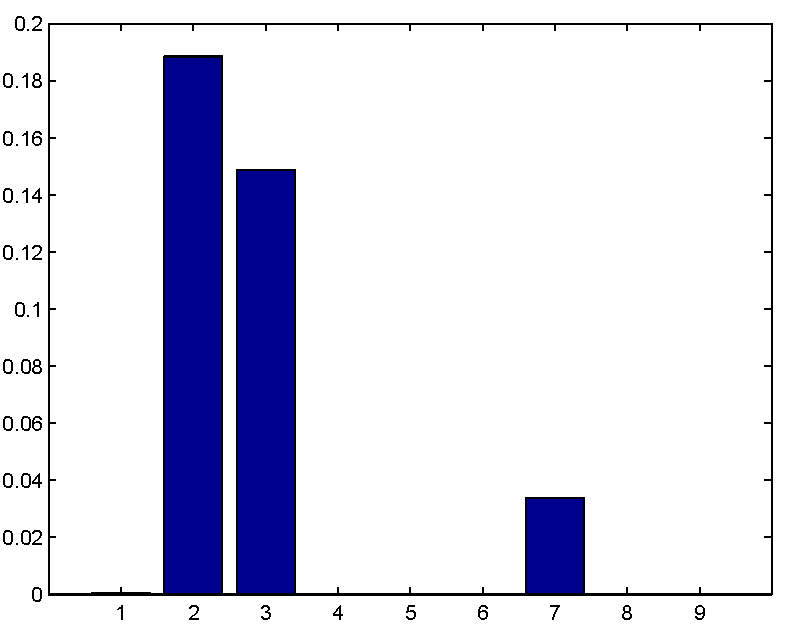
\includegraphics[width=0.4\textwidth]{../diagrams/supplMocapScalesRbf}
	\label{fig:suppMocap1}
}
\subfigure[]{
	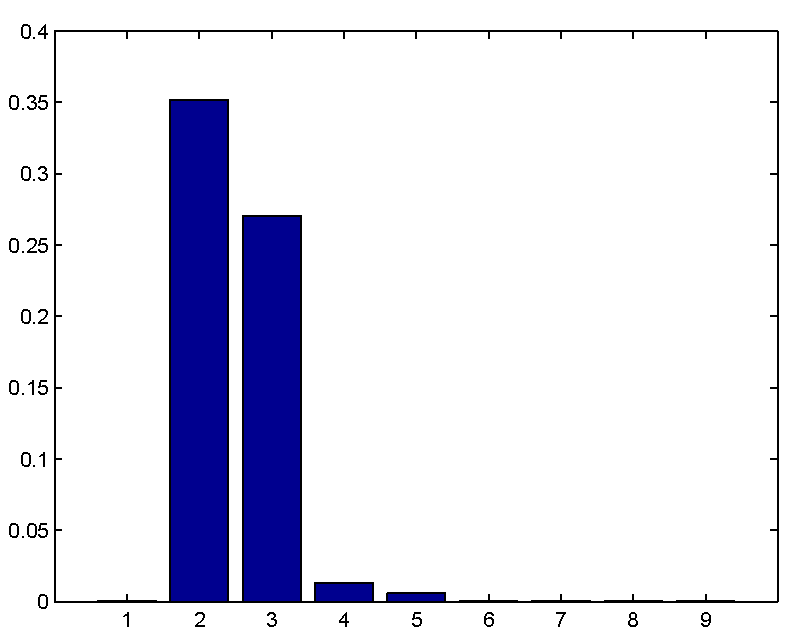
\includegraphics[width=0.4\textwidth]{../diagrams/supplMocapScalesMatern}
	\label{fig:suppMocap2}
}
\end{center}
\caption{\small{
The values of the scales of the ARD kernel after training on the motion capture dataset using the RBF (fig: \subref{fig:suppMocap1}) and the Matern (fig: \subref{fig:suppMocap2}) kernel to model the dynamics for VGPDS. The scales that have zero value ``switch off'' the corresponding dimension of the latent space. The latent space is, therefore, 3-D for \subref{fig:suppMocap1} and 4-D for \subref{fig:suppMocap2}. Note that the scales were initialized with very similar values.
}
}
\label{fig:supplMocap1}
\end{figure}


\begin{figure}[ht]
\begin{center}
\subfigure[]{
	%\includegraphics[width=0.48\textwidth]{diagrams/supplMocapBody23GpdsRbf}
	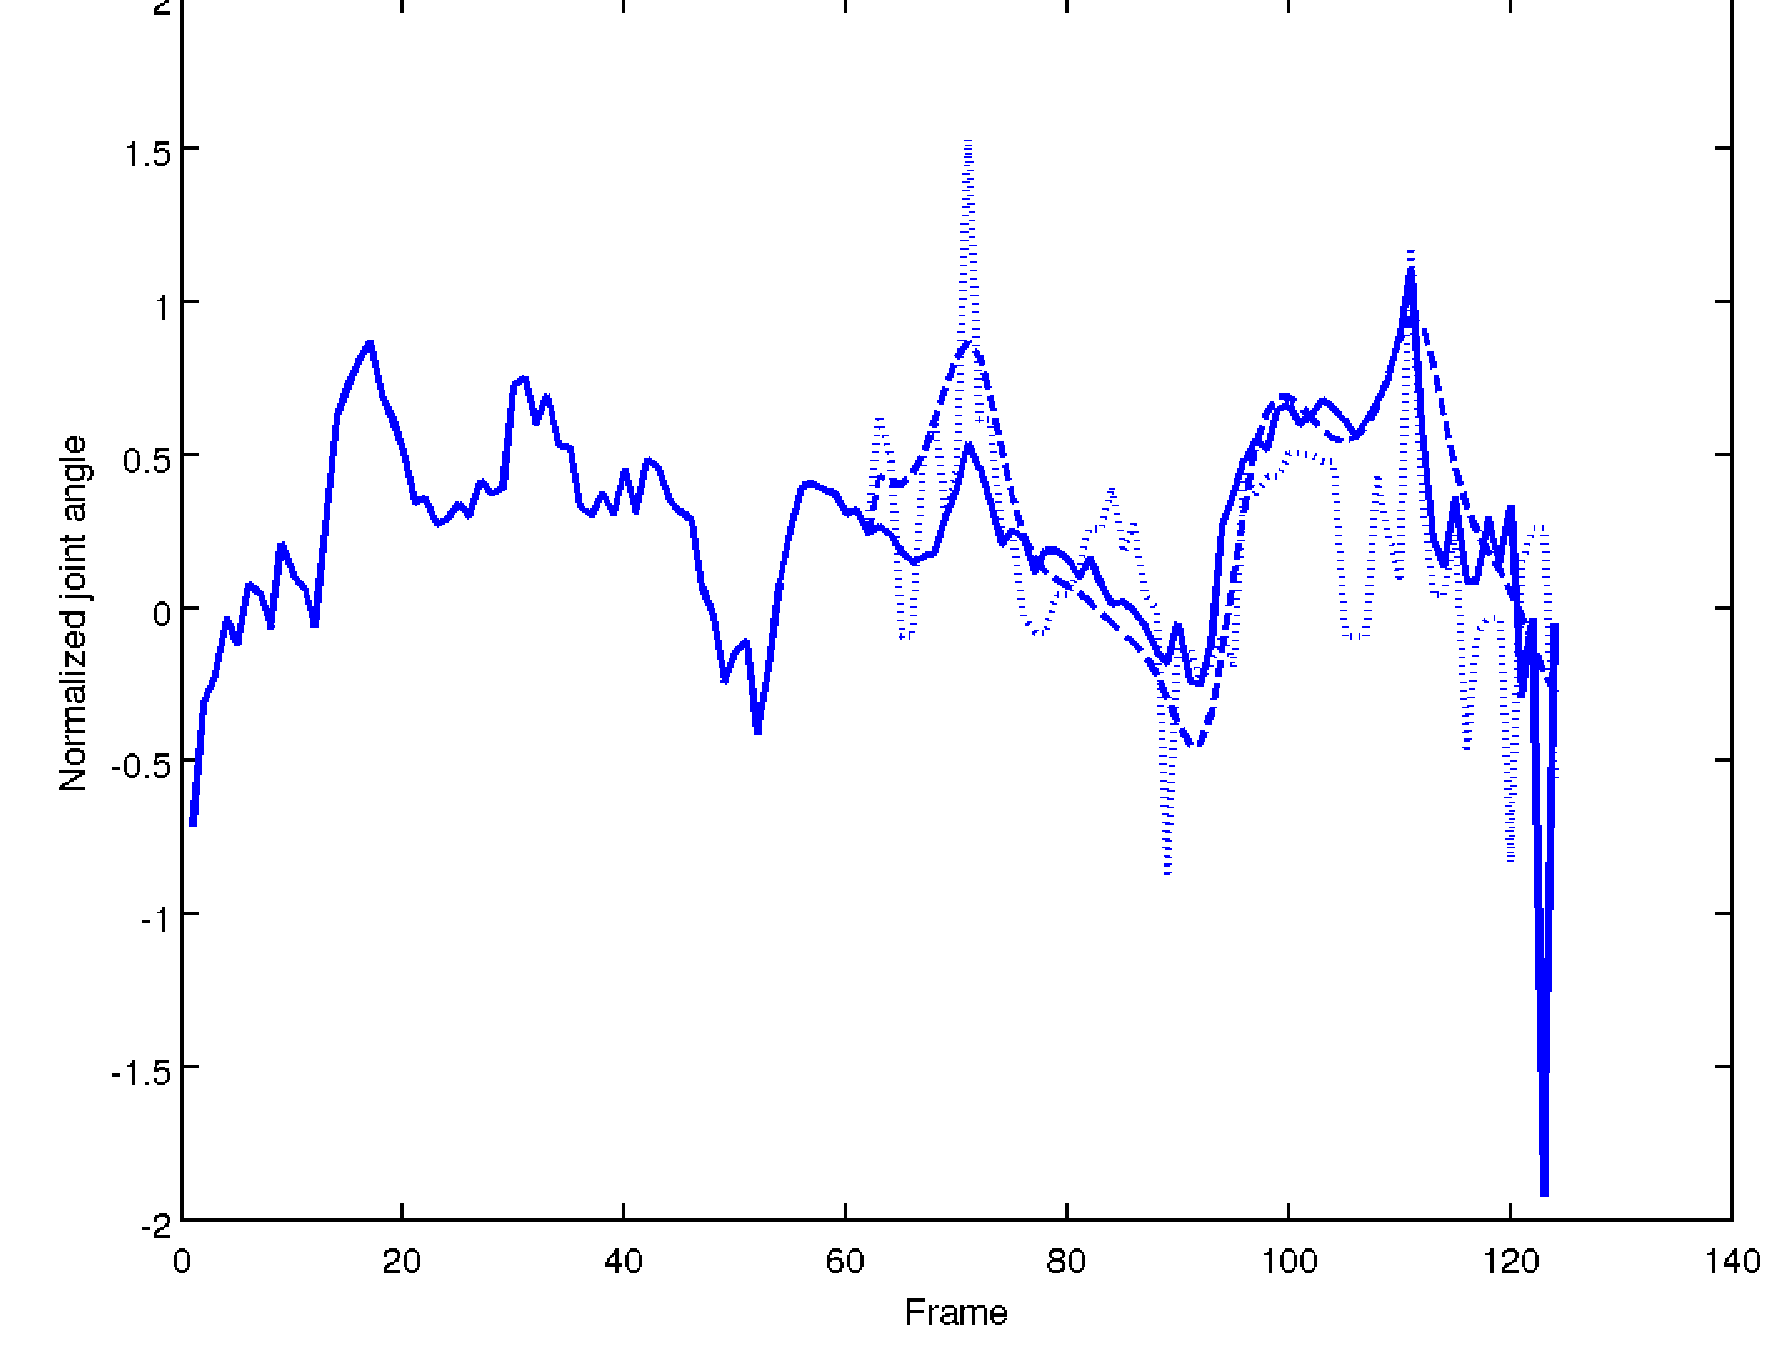
\includegraphics[width=0.48\textwidth]{../diagrams/supplMocapBody28GpdsMatern}
	\label{fig:suppMocap3}
}
\subfigure[]{
	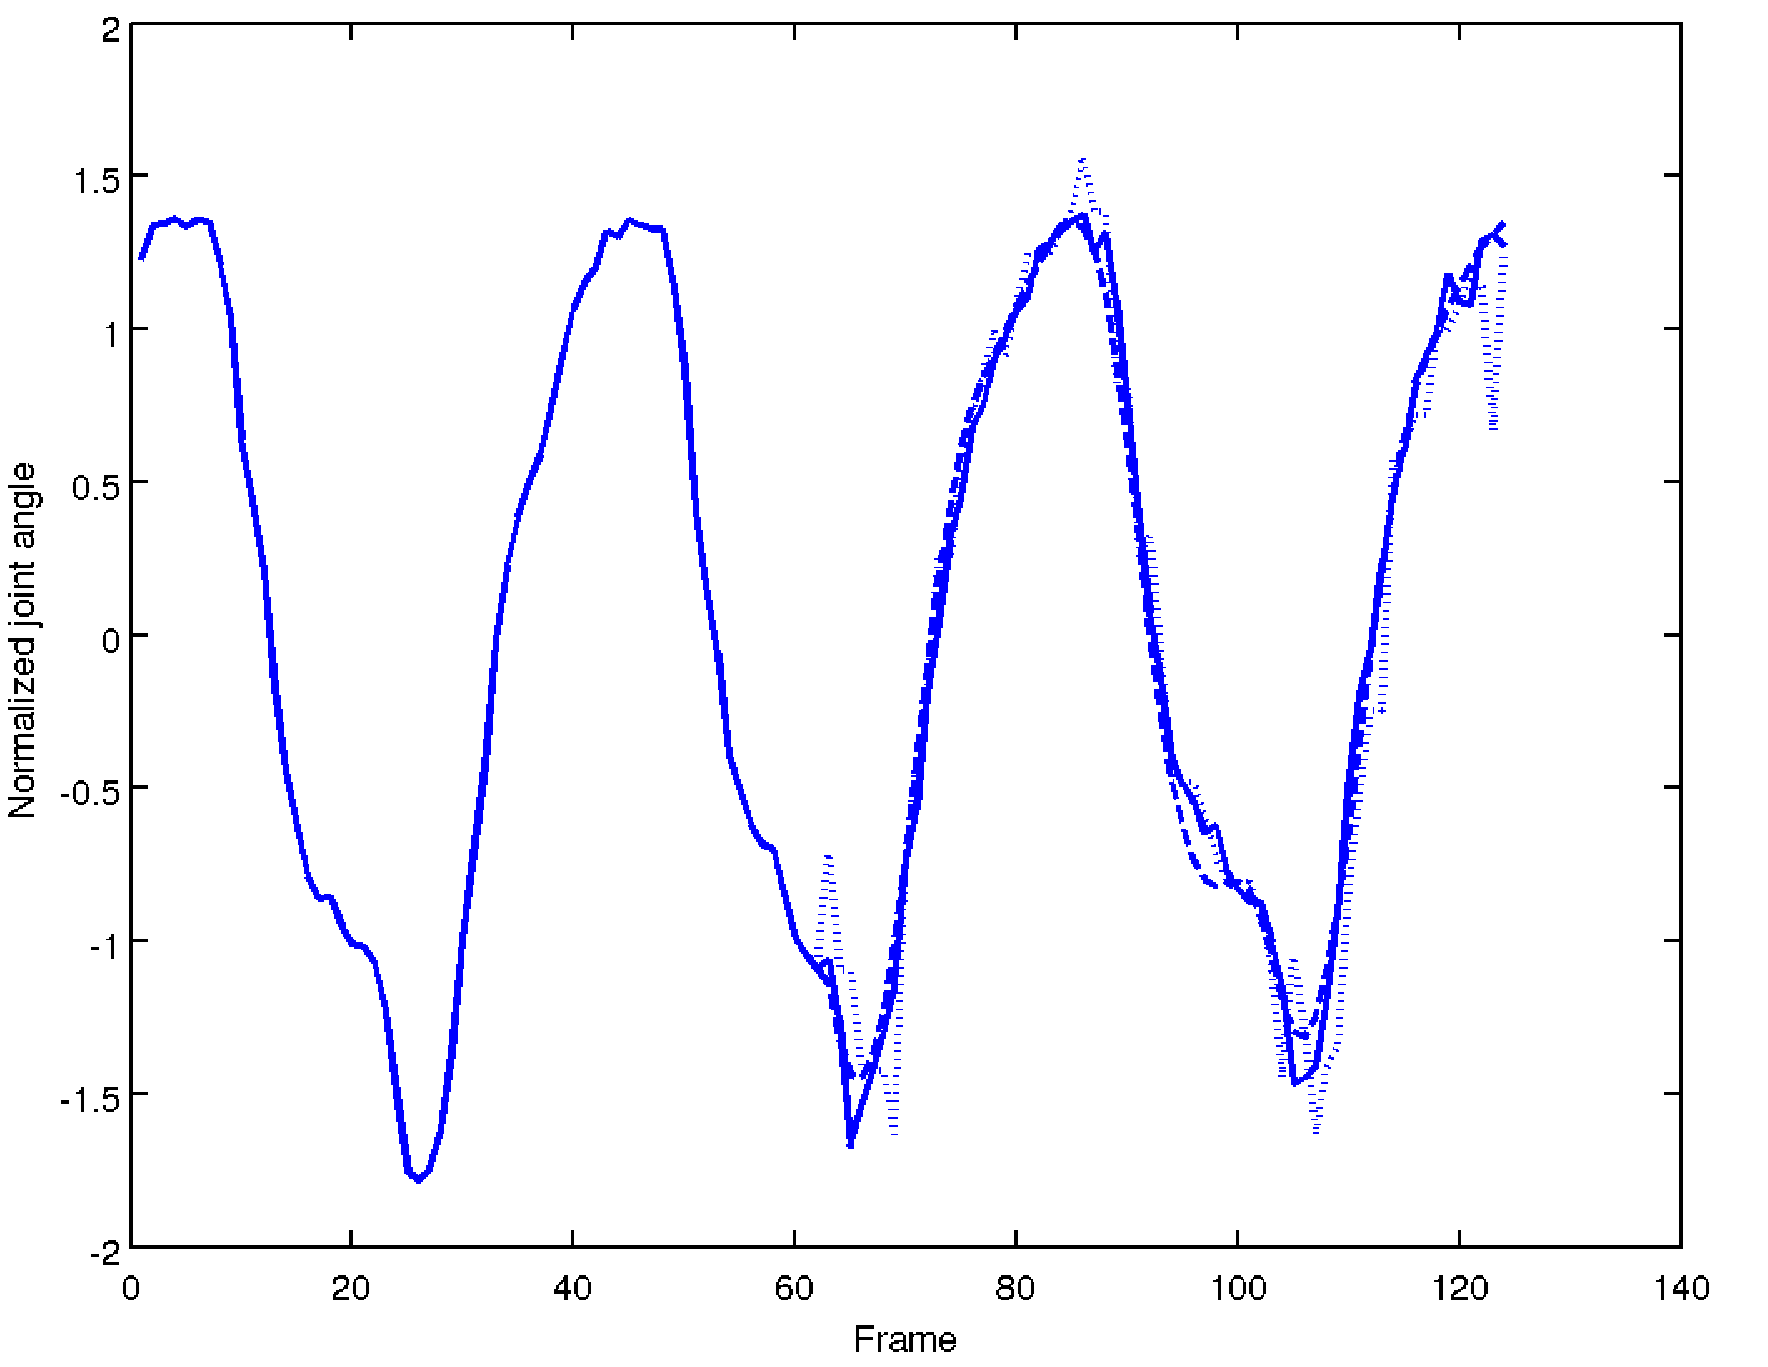
\includegraphics[width=0.48\textwidth]{../diagrams/supplMocapLeg5GpdsMatern}
	\label{fig:suppMocap4}
}
\end{center}
\caption{\small{
The prediction for two of the test angles for the body (fig: \ref{fig:suppMocap3}) and for the legs part (fig: \ref{fig:suppMocap3}). Continuous line is the original test data, dotted line is nearest neighour in scaled space, dashed line is VGPDS (using the RBF kernel for the body reconstruction and the Matern for the legs).
}
}
\label{fig:supplMocap2}
\end{figure}








\end{document}

% }
